
\chapter{Syntax와 Grammar}
\label{chap:SyntaxGrammar}
똑같은 한글 글자로 된 우리말 단어를 접하더라도 각자의 배경에 따라
그 용어를 해석하는 바가 달라진다. `정의'를 영어로 뭐냐고 물어보았을 때
justice라고 대답하면 문과, definition이라고 대답하면 이과 출신이라는
고전 유머를 한번쯤 들어 보았을 것이다. 참고로,
justice를 뜻하는 정의(正義)와 definition을 뜻하는 정의(定義)는
첫글자의 다른 한자인 동음이의어이므로 같은 어원에서 비롯된
분야에 따라 다른 다양한 의미로 전용되는 다의어는 아니다.
컴퓨터 분야에서 접할 수 있는 다의어의 예를 들자면 운영체제에서
어떤 작업을 담당하는 프로세스가 기존 작업의 일부 혹은 추가로
처리해야 할 작업을 따로 나눠 처리하기 위한 프로세스를 파생하는 경우,
원래 프로세스를 `부모'(parent) 파생된 프로세스를 `자녀'(child)로 부른다.
이는 일상생활에서 사용하는 `부모'와 `자녀'와 어느 정도 공통점은 있으나
상당히 다른 의미로 전용된 전문용어다.

반대로 같은 영어 단어를 분야에 따라 우리말로 다르게 옮기는 경우도 있다.
앞으로 이 책에서 자주 접하게 될 용어인
syntax를 우리말로 옮겨보라고 했을 때 주로
`문법'으로 옮긴다면 컴퓨터 관련 전공자로,
일관되게 `구문(론)' 혹은 `통사(론)'으로 옮기되 절대로 `문법`으로
옮기지는 않는다면 언어학 등 어문계열 관련 전공자로 판단할 수 있을 것이다.
컴퓨터과학의 프로그래밍언어 분야에서는 언어학에서부터 쓰던 전문용어를
도입해서 활용하고 있는데 언어학에서와는 약간씩 다르게 번역되거나
활용되기도 하므로 이런 용어들을 미리 정리하고 넘어가자.


\section{Syntax와 Grammar를 우리말로 옮기면?}
\index{syntax|see{문법}}%
\index{syntax|see{구문}}%
\index{grammar|see{문법}}%
\index{구문|see{syntax}}%
\index{문법|see{syntax}}%
\index{문법|see{grammar}}%
2009년에 출판된 영한사전\cite{OxEKdict}에서 syntax와 grammar를 찾아보면 다음과 같다.
\begin{quote}
    \textbf{syntax} 명사[U] \vspace{-1ex}
    \begin{enumerate}\tightlist
    \item{} [언어] 구문론, 통사론 (참고어: morphology)
    \item{} [컴퓨터] (컴퓨터 언어의) 문법
    \end{enumerate}
    \textbf{grammar} 명사 \vspace{-1ex}
    \begin{enumerate}\tightlist
    \item{} [U] 문법 (참고어: generative grammar)
    \item{} [U] (개인의) 문법 (문법적 지식이나 언어 사용)
    \item{} [C] 문법책
    \end{enumerate}
\end{quote}

실제로 십수 년 이전부터 우리말로 번역되거나 출간된 컴퓨터 관련 분야의
교과서, 논문, 보고서 등에서도 syntax를 `문법'으로 옮기는 경우가 많았고
지금도 마찬가지다. 예컨대, ``the syntax of the C programming language''는
보통 우리말로 ``C언어의 문법''이라고 옮긴다. 한편 ``syntax analysis''는
``문법분석''으로도 ``구문분석''으로 옮기기도 한다. 특히 자연언어를 컴퓨터로
다루는 자연언어처리 분야의 경우에는 ``구문분석''으로 옮기는 경우가 대부분이다.

다음으로 살펴볼 용어인 grammar는 분야에 관계없이 `문법'으로 옮기고 있다.
조금 이상하지 않은가? 언어학에서 `문법'과 `구문(론)'/`통사(론)'으로 구분하여
옮기던 grammar와 syntax를 어째서 컴퓨터과학의 프로그래밍언어 분야에 와서는
둘 다 `문법'으로 옮겨서 헷갈리게 만드는 것일까? 전문용어는 해당 분야 안에서는
하나의 개념에 대응해야 한다는 일의성 원칙에도 어긋나며, 유사/관련 분야에 걸쳐
일관성/통일성이 있어야 한다는 관점에서도 그다지 좋지 못한 선택이다.
프로그래밍언어 분야에서 syntax를 `문법'으로 옮기게 되었던 이유가 무엇인지
나름대로 미루어 짐작해 보자면 다음과 같지 않을까 생각한다.
\begin{enumerate}\tightlist
    \item 자연언어와 프로그래밍언어에서 syntax와 grammar의 상관관계
    \item 일의성, 일관성/통일성보다 친숙성을 우선시한 번역
\end{enumerate}

\index{syntax}%
\index{grammar}%
\index{문법}%
자연언어를 다루는 언어학에서는 syntax를 grammar의 일부분으로 인식하는 경우가
대부분이지만, 프로그래밍언어 특성상 grammar를 활용하는 경우는 대부분
syntax를 처리하기 위해서이다. 즉, 자연언어에서는 grammar라고 하면 syntax를
포함한 여러 가지를 함께 생각할 수밖에 없지만 프로그래밍언어에서는 grammar라고
하면 거의 syntax만을 떠올리는 것이 보통이다 (\ref{sec:NatProgSyn}절 참고).
따라서 일의성, 일관성/통일성은 좀 떨어지지만 일상생활에서 `구문'이라는
단어보다는 `문법'이라는 단어가 더 익숙하기 때문에 과거에 프로그래밍언어 관련
전문용어를 번역할 때 grammar와 겹치는 것을 모르지 않았겠지만 그냥 똑같이
`문법'으로 옮겼던 것 같다.

지금은 인공지능 기술의 발달로 컴퓨터 관련 분야에서도 자연언어처리의 활용이
크게 늘어나는 추세이다. 컴퓨터 관련 분야에서 프로그래밍언어 분야에 비해
적은 응용 부분을 차지하던 자연언어처리가 지금은 매우 커지고 있다는 점을
생각한다면 프로그래밍언어 분야에서도 앞으로 syntax를 `문법'으로 옮기지 않고
`구문'으로 옮기는 것이 장기적으로는 더 좋은 선택일지 모르겠다. 하지만
지금까지는 프로그래밍언어 관련해서는 syntax를 `문법'으로 옮기는 경우가 더
많으므로 이 책에서도 syntax를 `문법'으로 주로 옮기되 grammar인지 syntax인지
분명히 밝힐 필요가 있다고 생각되는 경우에는 영문 용어와 병기하도록 하겠다.

\section{자연언어, 인공언어, 형식언어}
\index{자연언어|see{natural language}}%
\index{natural language|see{자연언어}}%
\index{언어!자연언어|see{natural language}}%
\index{language!natural language|see{자연언어}}%
자연언어(natural/ordinary language)는 사람들끼리 의사소통을 위해 누가 만들었는지도 모르게
자연스럽게 생겨난 언어를 일컫는다. 한국어, 영어 등과 같은 대다수의 음성언어가
자연언어에 속한다. 또한 비음성언어 중에 자연언어로는 농아인들 사이에서 의사소통을
위해 생겨난 수어(sign language)가 있다.

\index{인공언어|see{artificial language}}
\index{언어!인공언어|see{artificial language}}
\index{artificial language|see{인공언어}}
\index{language!artificial language|see{인공언어}}
인위적으로 만들어진 인공언어(artificial/constructed/invented/planned language)는
자연언어와 대비되는 개념이다. 대표적인 예로는 특정 문화 및 국적에 덜 종속적인
국제어를 표방하는 에스페란토(Esperanto)를 들 수 있다. 또한 톨킨 세계관에서
고대 엘프어인 꿰냐(Quenya)나 스타트랙 세계관에서 전투적 외계 종족인 클링온(Klingon)의
언어 등과 같이 예술작품 안 가상의 세계에 더 생생한 설정을 불어넣기 위해 만들어져
창작 의도가 실생활에 활용할 목적과는 동떨어진 가공의 언어들도 인공언어로 분류할 수 있다.

\index{형식언어|see{formal language}}
\index{언어!형식언어|see{formal language}}
\index{formal language|see{형식언어}}
\index{language!formal language|see{형식언어}}
형식논리, 형식언어, 계산이론, 프로그래밍언어 등의 분야에서 주로 다루는
형식언어(formal language)란 어떤 언어에 속하는 문장의 구성 방법이나
구성된 문장에 부여되는 의미를 정확한 논리적/수학적 규칙에 따라 모호함 없이
정의되는 언어를 말한다. 따라서 정해진 규칙에 따라 컴퓨터로 처리되어 실행되는
프로그래밍언어도 형식언어의 일종이다. 컴퓨터에서 실행할 것을 염두에 두고
만들어진 프로그래밍언어가 나오기 전부터 형식언어는 존재했다.
논리학에서 특정 논리 기호와 연결사로 이루어진 논리문(logical statements)이나
수학에서 특정 상수, 변수, 연산자로 이루어진 산술식(arithmetic expressions)
등이 그 사례다. 또한 음의 높낮이와 지속되는 길이를 나타내는 음표로 이루어진
악보도 형식언어의 일종으로 볼 수도 있다. 그러한 형식언어도 필요하다면
컴퓨터에 옮겨 처리할 수 있으므로 프로그래밍언어의 일종으로 취급해도
틀린 개념은 아니다. 따라서 넓은 의미의 `프로그래밍언어'는 `형식언어'와도
같은 개념으로 사용한다. 이런 넓은 의미에서 인류 역사에서 일찍이 등장한
프로그래밍언어의 예로 고대 주판(그림\;\ref{fig:RomanAbacus})에 올려놓은
작은 돌의 배열을 들 수도 있겠다.

\begin{figure}[b]\center
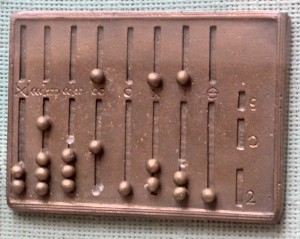
\includegraphics[scale=0.5]{RomanAbacusRecon.jpg}
\caption{로마시대 휴대용 주판 (복제품)\label{fig:RomanAbacus}\\
         \quad{\scriptsize (사진 출처: 위키미디어 공용)} }
\end{figure}

자연언어와 인공언어의 구분은 사람들끼리의 일상적인 의사소통을 위한 언어를
분류할 때 주로 사용하는 개념이다. 애초에 형식언어가 아닌 맥락에서 나온 개념이다.
형식언어도 인위적으로 만들었다는 점에서는 인공언어의 정의에도 부합하는 면이 있으나
그런 맥락에서는 사용하는 것은 일반적이지 않다. 그러니까 프로그래밍언어를
인공언어라고 해도 틀린 이야기는 아니지만 맥락에 따라 조금 어색한 표현일 수도 있다.
프로그래밍언어는 형식언어라고 이야기하는 것이 더 일반적인 표현이다.

컴퓨터 관련 분야에서 형식언어에 대비되는 개념, 즉 사람들끼리의 일상적인
의사소통을 위한 자연언어와 인공언어를 아우르는 용어는 그럼 무엇일까?
그냥 모두 `자연언어'라고 한다. 왜냐하면 형식언어는 사람들끼리 일상적인
의사소통에 사용하는 언어들과는 워낙 그 특성이 동떨어져 있기 때문이다.
즉, 자연언어와 인공언어의 거리가 서울 부산 정도라면 형식언어는 달나라나
목성쯤에 있다고 비유할 수 있겠다. 인공지능 등의 기술로 한국어나 영어 등의
자연언어를 다루는 분야를 자연언어처리(natural language processing, NLP)라고 한다.
같은 기술로 에스페란토와 같은 인공언어를 처리한다 인공언어처리라고 부르지 않고
그냥 똑같이 자연언어처리로 취급할 따름이다.

\section{자연언어와 프로그래밍언에서 Syntax의 비중}
\label{sec:NatProgSyn}
\index{syntax}%
\index{구문}%
언어학에서 음성 기반의 자연언어를 다룰 때는
작은 단위부터 큰 맥락까지 아래와 같이 다섯 같은 단계로 나눠 설명한다고 한다.
\begin{enumerate}\tightlist
    \item 음운론(phonology):
    소리의 단위인 음운을 다루는 이론.
    \item 형태론(morphology):
    의미의 단위인 형태소로 어휘를 구성하는 이론.
    \item 구문론(syntax):
    어휘로 문장을 구성하는 이론.
    \item 의미론(semantics):
    어휘나 문장이 갖는 의미에 대한 이론.
    \item 화용론(pragmatics):
    상황/문맥에 따른 어휘/문장의 활용을 다루는 이론.
\end{enumerate}
자연언어에서 문법(grammar)이란 음운론, 형태론, 구문론을 포괄하며 경우에 따라
의미론도 포함한다 \cite{IntroEngSem}. 자연언어 문장에서는 통사론적으로 같은
분류에 속하는 단어끼리도 원래의 단어를 다른 단어로 바꿔쳤을 때 그 의미의
차이에 따라 잘못된 문장으로 취급될 수도 있기 때문이다. 물론 자연언어에서도
구문론/통사론(syntax)이 문법(grammar)에서 다루는 핵심적인 부분이지만
그 외의 다른 요소들도 무시하지 못할 비중을 차지한다. 정리하면,
언어학에서 syntax는 grammar가 다루는 영역 중의 하나이므로
둘을 같은 우리말 용어로 옮겨 놓는다면 대단히 혼란스러울 것이다.

\index{syntax}
\index{문법}
음성에 기반하지 않는 형식언어에서 음운론은 애초부터 논외이다.
프로그래밍언어 문법(syntax)의 대부분은 형식언어를 분류한 촘스키 계층
중에서 문맥자유언어(context-free language, CFL)에 해당한다.
문맥자유언어는 문법적으로 올바른 문장인지 판단하는 데 있어 의미나 맥락이
영향을 미치지 않으므로 형태론과 구문론만 고려하면 된다. 그런데 형식언어를
정의할 때에는, 예전부터 쓰던 어휘를 유지/계승해야 하는 자연언어와 달리, 
활용 목적에 알맞은 어휘를 새롭게 정하면 그만이므로 상대적으로 형태론의
비중도 미미하다. 따라서 프로그래밍언어에서 grammar는 syntax에 대한 내용을
주로 다루는 것이 당연하다. 즉, 프로그래밍언어에서는 syntax외에 grammar에서
다룰 내용이 거의 없으므로 둘 다 똑같이 `문법'으로 옮기더라도 그렇게 크게
혼란스럽지는 않을 것이다.

지금까지는 자연언어의 맥락에서 나온 용어들이 프로그래밍언어에서는 어떻게
그 번역이나 활용이 달라졌는지에 대해서 주로 이야기했다. 그런데 사실
형식언어에서 syntax와 grammar의 관계는 자연언어에서와는 조금 다른 관점에서
정리할 필요가 있다. 이에 대해서는 이어지는 절에서 좀 더 이야기하기로 하자.

\section{형식언어이론에서 Syntax와 Grammar의 관계}
\label{sec:FormalLangSG}
\index{syntax}%
\index{grammar}%
\index{형식언어!syntax}%
\index{형식언어!grammar}%
\index{formal language!syntax}%
\index{formal language!grammar}%
\index{형식언어이론|see{formal language theory}}%
\index{formal language theory|see{형식언어이론}}%
형식언어이론(formal language theory, FLT)은 문장(정확히는 문자열)의 생김새(syntax)만을
대상으로 하며 그 뜻(semantics)은 생각하지 않는다. 형식언어이론에서
\index{언어|see{language}}%
\index{language|see{언어}}%
`언어'(language)란 단순히
\index{string|see{문자열}}%
\index{문자열|see{string}}%
문자열(string)의 집합으로 정의된다. 문자열은 언어마다 미리 정해놓은 유한한 종류의
기호(symbol)를 한줄로 유한한 개수만큼 늘어놓아 만들어지며, 늘어놓은 기호의 개수가
바로 문자열의 길이가 된다. 형식언어에서 기호는 자연언어의
\index{어휘|see{lexeme}}%
\index{lexeme|see{어휘}}%
어휘(lexeme)에 대응되는 부분이다.
자연언어의 어휘는 의미의 최소단위인 형태소로 이루어지는 반면,
형식언어의 기호는 더 이상 쪼개지지 않고 의미가 부여되지 않는
원자적이고 추상적인 어휘에 해당한다.

이해를 돕기 위해 흑돌(\txtbullet)과 백돌(\txtcircle) 두 종류의 기호를 사용하는 형식언어
$L = \{\, {\txtbullet\txtcircle}
      ,\, {\txtbullet\txtcircle}{\txtbullet\txtcircle}
      ,\, {\txtbullet\txtcircle}{\txtbullet\txtcircle}{\txtbullet\txtcircle}
      ,\, {\txtbullet\txtcircle}{\txtbullet\txtcircle}{\txtbullet\txtcircle}{\txtbullet\txtcircle}
      ,\, {\txtbullet\txtcircle}{\txtbullet\txtcircle}{\txtbullet\txtcircle}{\txtbullet\txtcircle}{\txtbullet\txtcircle}
      ,\, \ldots
   \,\}$을 생각해 보라.
사실 기호의 표기상 그 모양이 바둑의 흑돌과 백돌처럼 보이기도 하기 때문에
편의상 그냥 `흑돌'과 `백돌'이라 부를 뿐 바둑과 관련된 의미를 부여하려는
것은 아니다. `꽉찬 동그라미'와 `빈 동그라미' 등으로 불러도
$L$의 정의는 젼혀 달라질 것이 없다. (더 나아가,
\txtbullet,\txtcircle 대신 $a$,$b$ 등으로 서로 구분되는
다른 어떤 두 기호라도 탐구하려는 형식언어의 본질이 달라지지는 않는다.)
이 언어에서 올바른 (즉, $L$의 원소인) 문자열의 특징을 설명하자면,\vspace{-1ex}
\begin{itemize}\tightlist
    \item[-] 가장 왼쪽 기호는 흑돌이고 가장 오른쪽 기호는 백돌이며
    \item[-] 같은 색 돌이 연속해 나타나지 않고 흑돌과 백돌이 번갈아 나타난다.
\end{itemize}
이와 같이 $L$에 속하는 문자열의 모양새가 어떠해야 하는지 제시하는 내용이
바로 언어 $L$의 syntax에 대한 표현이다. 이러한 내용은 언어 $L$의 고유한
성질을 알려줄 뿐이며 구체적으로 $L$에 속하는 문자열을 어떤 방법으로 어떤
과정을 거쳐 만들어내는지에 대해서까지 나타나 있지는 않다.

그렇다면 이번에는 좀 더 구체적으로 문자열 \txtbullet\txtcircle\txtbullet\txtcircle를
만들어내는 방법을 생각해 보자. 굉장히 다양한 방법으로 만들어내는 것이 가능하며
그 중에서 다음의 몇 가지만 살펴보겠다.
\begin{enumerate}
    \item
    \fbox{\fbox{\fbox{\fbox{\!\txtbullet\!}\,\txtcircle\!}\,\txtbullet\!}\,\txtcircle\!}
    왼쪽 끝의 흑돌 하나로부터 오른쪽으로 하나씩 이어붙여서
    \item
    \fbox{\!\txtbullet\,\fbox{\!\txtcircle\,\fbox{\!\txtbullet\,\fbox{\!\txtcircle\!}}}}
    오른쪽 끝의 백돌 하나로부터 왼쪽으로 하나씩 이어붙여서
    \item
    \fbox{\fbox{\!\fbox{\!\txtbullet\!}\,\txtcircle\!}\,\fbox{\!\fbox{\!\txtbullet\!}\,\txtcircle\!}}
    흑돌 백돌 하나씩의 길이 2인 문자열이 두 번 반복되는 구조로
\end{enumerate}
$L$의 고유한 성질인 syntax를 표현하는 방식의 하나인 grammar를 어떻게 작성하느냐에
따라 만들어지는 결과물은 모두 \txtbullet\txtcircle\txtbullet\txtcircle로 같지만
그 문자열이 구성되는 방법과 만들어지는 과정이 달라질 수 있다. 즉, 같은 언어를 표현하는
서로 다른 grammar는 해당 언어에 속하는 문자열을 모두 만들어내므로 최종 결과물로 나오는
문자열들은 같지만, 만들어내는 구체적인 방식과 과정에는 차이가 있을 수 있다는 것이다.

지금까지 형식언어에서 syntax와 grammar가 어떤 식으로 관련된 개념인지 정리해 보았다.
형식언어의 계층적 분류 및 형식언어의 문법(grammar)에 대한 조금 더 자세한 이야기는
요점정리 후에 이어지는 다음 장에서 이어가기로 하자.

\section*{요점정리}
\begin{itemize}[itemsep=0pt]
    \item 프로그래밍언어란 좁은 의미에서는 기계(컴퓨터)에서 실행할 것을
    염두에 두고 만들어진 형식언어의 일종이지만 넓은 의미에서는 형식언어를
    모두 아우르는 개념이다.
    \item
    컴퓨터 분야에서 (형식언어 말고) `자연언어'라고 하면
    언어학에서 자연언어와 인공언어를 함께 아우르는 개념이다.
    \item
    프로그래밍언어 관련해서는 syntax와 grammar를 모두 `문법'이라고
    번역하는 경우가 많다. 둘은 관련된 개념이지만 구분할 필요가 있다.
    \item
    자연언어에서는 grammar가 다루는 여러 영역 중 하나가 syntax이다.
    \item
    형식언어의 syntax란 올바른 문자열의 모양새가 어떠해야 하는지 제시하는
    내용으로 특정 형식언어의 고유한 성질에 해당한다.
    \item
    형식언어의 grammar는 올바른 모양의 문자열을 만들어내기 위해
    사용하는 설계/시공 방법에 비유할 수 있다.
\end{itemize}


\chapter{형식언어이론}
\index{형식언어이론}
\index{formal language theory}
형식언어이론에서는 어휘를 원자적 기호(symbol)로 추상화하여 의미를 부여하지 않으며,
기호의 나열로 이루어진 문자열(string)의 모양새(syntax)만을 기준으로 원하는 문자열을
골라 모아놓은 집합을 `언어'(language)로 규정한다. 문법(grammar)은 어떤 언어에 속하는
문자열을 만들어내는 과정을 안내하는 구체적인 규칙들로 이루어진다. 이런 문법을
어떤 식으로 정의하고 활용하는지 이 장에서 조금 더 자세히 소개한다. 그리고
문법(grammar)과 언어(language)의 모호성이 어떠한 개념인지 알아본다.
프로그래밍언어의 어휘(lexeme)와 구문(syntax)을 처리하는 데에도 형식언어이론을
활용하는데, 이런 활용에 있어서는 모호성을 피하는 것이 바람직하다.
프로그래밍언어에도 어휘분석(lexical analysis)보다 구문분석(syntax analysis)이
한층 더 복잡한 문제다. 따라서 어휘분석에 활용되는 형식언어보다 구문분석에 
활용되는 형식언어가 더 다루기 힘든 복잡한 성질을 가지고 있을 것이다.
형식언어의 복잡도에 따라 분류한 촘스키 계층 구조에 대해서도 소개한다.

이 책은 프로그래밍언어 분야에서 기본적으로 알아야 할 개념을 익히는
것을 목표로 하므로, 여기서는 형식언어이론을 체계적으로 다루기보다는
프로그래밍언어의 이해와 관련해 도움이 될만한 내용 위주로 간략하고 직관적으로 소개한다. 
형식언어이론에 전반에 대해 더 체계적으로 알아보려면 형식언어, 오토마타, 계산이론
등을 주제로 하는 교재\cite{Sipser2013,Hopcroft2007}를 참고하라.

\section{형식언어의 문법에 따른 문자열 생성}
\label{sec:GenGrammar}
\index{문법}%
\index{grammar}%
\index{형식문법|see{formal grammar}}%
\index{formal grammar|see{형식문법}}%
형식언어의 문법(grammar)을 형식언어를 다룬다는 점을 강조하여 형식문법(formal grammar)이라
부르기도 한다. 형식언어이론에서 형식문법을 작성하는 표준적인 방식은 문자열을
만들어 나가는 과정을 안내하는 생성규칙을 작성하며 이러한 방식로 문법을
표현한 것을
\index{생성문법|see{generative grammar}}%
\index{generative grammar|see{생성문법}}%
\index{형식문법!생성문법}%
\index{formal grammar!generative grammar}%
생성문법(generative grammar)이라고 한다. 형식언어의 문법
$G = \langle\, \Sigma, N, S, R \,\rangle$의 네 가지 요소는 다음과 같다.\vspace{-1ex}%
\index{단말 기호|see{terminal symbol}}%
\index{terminal symbol|see{단말 기호}}%
\index{비단말 기호|see{nonterminal symbol}}%
\index{nonterminal symbol|see{비단말 기호}}%
\index{시작 기호|see{start symbol}}%
\index{start symbol|see{시작 기호}}%
\index{생성규칙|see{production rule}}%
\index{production rule|see{생성규칙}}%
\index{형식문법!생성문법!단말 기호}%
\index{형식문법!생성문법!비단말 기호}%
\index{형식문법!생성문법!시작 기호}%
\index{형식문법!생성문법!생성규칙}%
\index{formal grammar!generative grammar!terminal symbol}%
\index{formal grammar!generative grammar!nonterminal symbol}%
\index{formal grammar!generative grammar!start symbol}%
\index{formal grammar!generative grammar!production rule}%
\begin{itemize}\tightlist
    \item[$\Sigma$]: 생성된 문자열에 나타나는 단말 기호(terminal symbol)의 집합
    \item[$N$]: 생성 과정에 추가로 나타나는 비단말 기호(nonterminal symbol)의 집합
    \item[$S$]: 생성의 시작을 나타내는 시작 기호(start symbol) (단, $S\in N$)
    \item[$R$]: 생성규칙(production rule)의 집합.
\end{itemize}

\index{symbol|see{기호}}
\index{기호|see{symbol}}
여기서 문법에 대해 구체적으로 소개하기 전에 형식언어란 문자열의 집합이며
문자열은 추상적인 어휘에 해당하는 `기호'로 이루어진다고 언급했는데,
그때 말한 기호가 바로 단말 기호에 해당한다.
그래서 단말 기호는 문법(grammar)과는 별개로 언어의 정의만으로도 결정된다.
앞서 \ref{sec:FormalLangSG}절에서 예시로 들었던 흑돌과 백돌 기호를 사용한
언어에서 단말 기호의 집합 $\Sigma = \{\txtbullet, \txtcircle\}$이다.
최종 문자열을 생성하기 위한 추가적인 과정을 이어갈 필요가 없다는 뜻에서
`단말'이라는 표현을 쓴다고 이해해도 무방하다.

비단말 기호란 문자열의 생성 과정에서 단말 기호 이외에 추가로 나타나는
다른 기호를 말한다. 형식문법에서는 비단말 기호 중 하나를 시작 기호로
정해 놓아야 하므로 비단말 기호의 집합 $N$은 공집합일 수 없다. 시작 기호는
생성할 전체 문자열을 대표하는 기호로, 하나의 시작 기호($S$)로부터 문법의
생성규칙에 따라 단계적으로 생성 과정을 거쳐 최종적으로는 단말 기호만으로
이루어진 문자열이 만들어지게 된다. 생성 과정의 중간 단계에서는 비단말 기호만으로
이루어지거나 비단말과 단말 기호가 함께 나타나는
\index{확장된 문자열|see{intermediate string}}%
\index{intermediate string|see{확장된 문자열}}%
\index{문자열!확장된 문자열}%
\index{string!intermediate string}%
확장된 문자열(intermediate string)의 개념이 필요하다.
문자열을 구성하는 바탕이 되는 기호의 집합을
\index{알파벳|see{alphabet}}%
\index{alphabet|see{알파벳}}%
\index{형식언어!알파벳}%
\index{formal language!alphabet}%
알파벳(alphabet)이라 부른다.
최종 문자열의 알파벳은 단말 기호 집합($\Sigma$)이며 확장된 문자열의 알파벳은
단말과 비단말 기호의 합집합($\Sigma\cup N$)이다. 참고로 알파벳이 $X$인
모든 문자열의 집합을 $X^{*}$라 표기한다. 이를테면
$x$가 단말 기호를 알파벳으로 삼는 문자열이고
$\alpha$가 단말과 비단말 모두를 알파벳으로 삼는 문자열이라는
설명 대신 $x\in\Sigma^{*}$이고 $\alpha\in(\Sigma\cup N)^{*}$라고 쓰면 된다.

문법에서 가장 핵심적인 내용은 $\alpha\to\beta$ 형태의
\index{생성규칙}%
\index{production rule}%
생성규칙(production rule)이다.
여기서 $\alpha$와 $\beta$는  $\Sigma\cup N$을 알파벳으로 하는 확장된 문자열인데,
단, $\alpha$는 길이 0인 빈문자열($\varepsilon$으로 표기)이 아니어야 한다
(즉, $\lvert\alpha\rvert>0$ 혹은 $\alpha\neq\varepsilon$).
시작 기호 하나로 이루어진 확장된 문자열 $S$로부터 시작해, 매 단계마다
문자열의 일부분(혹은 전체)가 화살표 왼쪽($\alpha$)과 일치하는 생성규칙
하나를 $R$에서 찾아 화살표 오른쪽($\beta$)의 내용으로 치환해 나가는 과정을
반복한다. 여러 생성규칙의 화살표 왼쪽이 일치하는 경우에는 어떤 것을 선택해도 된다.
치환 결과로 나온 문자열 $x$가 비단말 없이 단말 기호로만 이루졌다면
성공적으로 문자열을
\index{유도|see{derivation}}%
\index{derivation|see{유도}}%
유도(deriviation)한 것이며
$S\xRightarrow[\,G]{} \cdots \xRightarrow[\,G]{} x$ (단, $x\in\Sigma^{*}$)와 같이 표현한다.
만일 화살표의 왼쪽이 일치하는 생성규칙을 $R$에서 찾을 수 없다면
최종 문자열 유도에 실패한 상황으로 생성 과정을 더 이상 진행할 수 없게 된다.
이렇게 문법 $G$의 생성규칙에 따라 생성 가능한 모든 최종 문자열의 집합을
$\mathcal{L}(G)$로 표기한다.

\begin{figure}\centering
\begin{subfigure}[b]{0.4\textwidth}
\begin{align*}
G_1 & = \langle\, \Sigma, N_1, S_1, R_1 \,\rangle ~ \text{where}
\\ & \Sigma = \{\txtbullet,\txtcircle\}
\\ & N_1 = \{S_1,A_1\}
\\ & R_1 = \left\{
             \begin{array}{l}
             S_1 \to \txtbullet\,A_1 \,,\\
             A_1 \to \txtcircle\,S_1 \,,\\
             A_1 \to \txtcircle 
            \end{array}
           \right\}
\\ ~
\end{align*}
\end{subfigure}
\hfill
\begin{subfigure}[b]{0.35\textwidth}
\begin{align*}S_1
~\xRightarrow[\,G_1\!]{}~ & \txtbullet A_1
\\
~\xRightarrow[\,G_1\!]{}~ & \txtbullet \txtcircle\, S_1
\\
~\xRightarrow[\,G_1\!]{}~ & \txtbullet \txtcircle \txtbullet A_1
\\
~\xRightarrow[\,G_1\!]{}~ & \txtbullet \txtcircle \txtbullet \txtcircle
\\ ~
\end{align*}
\end{subfigure}
\hfill
\begin{subfigure}[b]{0.2\textwidth}\small
\begin{forest}
for tree={fit=tight, l sep-=.7em, l-=.7em}
  [$S_1$ [\txtbullet]
         [$A_1$ [\txtcircle]
                [$S_1$ [\txtbullet]
                       [$A_1$ [\txtcircle]]
                ]
         ]
  ]
\end{forest}\\
\end{subfigure}
\\
\begin{subfigure}[b]{0.4\textwidth}
\begin{align*}
G_2 & = \langle\, \Sigma, N_2, S_2, R_2 \,\rangle ~ \text{where}
\\ & \Sigma = \{\txtbullet,\txtcircle\}
\\ & N_2 = \{S_2,A_2\}
\\ & R_2 = \left\{
             \begin{array}{l}
             S_2 \to A_2\,\txtcircle \,,\\
             A_2 \to S_2\,\txtbullet \,,\\
             A_2 \to      \txtbullet
            \end{array}
           \right\}
\end{align*}
\subcaption*{grammar}
\end{subfigure}
\hfill
\begin{subfigure}[b]{0.35\textwidth}
\begin{align*}S_2
~\xRightarrow[\,G_2\!]{}~ & ~~~\; A_2\,\txtcircle
\\
~\xRightarrow[\,G_2\!]{}~ & ~~ S_2 \txtbullet \txtcircle
\\
~\xRightarrow[\,G_2\!]{}~ & A_2 \txtcircle \txtbullet\, \txtcircle
\\
~\xRightarrow[\,G_2\!]{}~ & ~ \txtbullet \txtcircle \txtbullet \txtcircle
\end{align*}
\subcaption*{derivation}
\end{subfigure}
\hfill
\begin{subfigure}[b]{0.2\textwidth}\small
\begin{forest}
for tree={fit=tight, l sep-=.7em, l-=.7em}
  [$S_2$ [$A_2$ [$S_1$ [$A_2$ [\txtbullet]]
                       [\txtcircle]
                ]
                [\txtbullet]
         ]
         [\txtcircle]
  ]
\end{forest}
\subcaption*{syntax tree}
\end{subfigure}
\caption{같은 언어에 대한 서로 다른 문법 $G_1$, $G_2$에 따른
         문자열의 유도(derivation) 및
         그에 대응되는 문법나무(syntax tree)
         \label{fig:OneLangTwoGrammar}
         }
\end{figure}

실제로 보기를 들어 설명하면 더 확실히 이해하는 데 도움이 될 것이다.
앞서 언급한 흑돌과 백돌을 기호로 하는 언어 
$L = \{\, \txtbullet\txtcircle
      ,\, {\txtbullet\txtcircle}{\txtbullet\txtcircle}
      ,\, {\txtbullet\txtcircle}{\txtbullet\txtcircle}{\txtbullet\txtcircle}
      ,\, \ldots
   \,\}$을 다시 생각해 보자.
언어 $L$의 문법 $G$를 정의한다는 말은 $L = \mathcal{L}(G)$를 만족하는 문법 $G$를 찾는
것과 같다. 한 언어의 문법은 유일하지 않고 여러 가지로 정의할 수 있다.
그림\;\ref{fig:OneLangTwoGrammar}에는 $L = \mathcal{L}(G_1) = \mathcal{L}(G_2)$인
언어 $L$의 서로 다른 두 문법 $G_1$과 $G_2$의 정의가 나타나 있다. (사실은
언어 $L$을 표현하는 문법을 얼마든지 더 많이 다양하게 정의할 수 있다.)
문자열을 유도(derivation)하는 생성 과정은 마치 수식의 결과를 유도하는
계산 과정과 비슷하다. 차이점은 수식 계산이 큰 식을 점점 작게 하나의 값으로
줄이는 방향으로 진행되는 반면, 문자열 생성은 하나의 시작 기호를 점점 길게
전개하여 최종 문자열이 만들어지는 방향으로 진행된다. 문자열을 유도(derivation)하는
생성 과정에서는 매 단계마다 중간 과정에 중복된 정보의 표시가 많다. 예를 들면
그림\;\ref{fig:OneLangTwoGrammar}의 $G_1$에 따른 유도 과정의 첫 단계에서
생성된 가장 왼쪽의 \textbullet가 이후 단계에서 반복적으로 표기된다.
순차적으로 작성된 유도(derivation) 과정 대신에 도식적인
\index{문법나무|see{syntax tree}}
\index{syntax tree|see{문법나무}}
문법나무(syntax tree)의
형태로 표현하면 중복된 기호의 표시가 줄어들어 한눈에 알아보기 좋다.

\index{문법나무!파스트리}%
\index{문법나무!유도나무}%
\index{문법나무!구체적문법나무}%
\index{syntax tree!parse tree}
\index{syntax tree!derivation tree}
\index{syntax tree!concrete syntax tree}
\index{파스트리|see{parse tree}}%
\index{parse tree|see{파스트리}}%
\index{유도나무|see{derivation tree}}%
\index{derivation tree|see{유도나무}}%
\index{구체적문법나무|see{concrete syntax tree}}
\index{concrete syntax tree|see{구체적문법나무}}
참고로 프로그래밍언어에서 다루는 문법나무는 두 종류가 있다.
지금까지 다룬 그림\;\ref{fig:OneLangTwoGrammar}에 나타난 종류의 문법나무를
유도나무(derivation tree), 파스트리(parse tree), 또는
구체적문법나무(concrete syntax tree) 등으로 부른다.
이와 상대되는 또 다른 종류의 문법나무는
추상/요약 문법나무(abstract syntax tree)인데
이에 대해서는 다음 장(\ref{sec:LexParse}절)에서 다루기로 한다.

\section{문법과 언어의 모호성}
\label{sec:ambiguous}
\index{모호한|see{ambiguous}}%
\index{ambiguous|see{모호한}}%
앞절에서 예시로 살펴본 형식언어의 문법은 문맥자유문법(context-free grammar, CFG)이며
문맥자유문법으로 표현할 수 있는 형식언어를 문맥자유언어(context-free language, CFL)로
분류한다. 이 절에서는 문맥자유문법과 문맥자유언어의 `모호성'이라는 개념에 대해 알아본다.
문맥자유문법이나 문맥자유언어가 무엇인지는 다음 절에서 소개할 것이므로
지금은 `문맥자유'는 생략하고 그냥 (문맥자유)문법과 (문맥자유)언어라고 이야기하겠다.

하나의 문자열에 대해 서로 다른 여러 가지 문법나무를 구성할 수 있으면
모호한 문법이다. 앞서 그림\;\ref{fig:OneLangTwoGrammar}에서 살펴본
문법 $G_1$과 $G_2$는 모호하지 않다. 문자열을 한쪽 끝에서부터 한 글자씩
늘려 가며 다른 쪽 끝까지 생성하는 과정은 유일하므로 문법나무도 하나로
결정될 수밖에 없다. 그런데 같은 언어를 표현하는 다른 문법 $G'$를
그림\;\ref{fig:ambG}에서와 같이 정의해 보자.
\begin{figure}\centering
\begin{subfigure}{0.45\linewidth}
\begin{align*}
G' & = \langle\, \Sigma, N', S', R' \,\rangle ~ \text{where}
\\ & \Sigma = \{\txtbullet,\txtcircle\}
\\ & N' = \{S'\}\cup N_1 \cup N_2
\\ & R' = \left\{\!\!
             \begin{array}{l}
             S' \to S_1 \,,\\
             S' \to S_2
            \end{array}
          \!\!\right\} \cup R_1 \cup R_2
\end{align*}
\end{subfigure}
\hfill
\begin{subfigure}{0.4\linewidth}\!\!\!\!\!\!\!\!
\begin{forest}
for tree={fit=tight, l sep-=.8em, l-=.8em}
[$S'$
  [$S_1$ [\txtbullet]
         [$A_1$ [\txtcircle]
                [$S_1$ [\txtbullet]
                       [$A_1$ [\txtcircle]]
                ]
         ]
  ]
] 
\end{forest}
~\quad~
\begin{forest}
for tree={fit=tight, l sep-=.8em, l-=.8em}
[$S'$
  [$S_2$ [$A_2$ [$S_1$ [$A_2$ [\txtbullet]]
                       [\txtcircle]
                ]
                [\txtbullet]
         ]
         [\txtcircle]
  ]
] 
\end{forest}
\end{subfigure}
\caption{모호한 문법 $G'$에 따른 같은 문자열에 대한 두 문법나무
         \label{fig:ambG}}
\end{figure}
문법 $G'$의 생성규칙은 $G_1$과 $G_2$의 생성규칙을 모두 포함하며
추가로 $G'$의 시작 기호에서 $G_1$의 시작 기호로 가는 규칙
($S'\to S_1$)과 $G_2$의 시작 기호로 가는 ($S'\to S_2$)으로
구성된다. 즉, $G'$에 따라 문자열 생성을 시작하면 $G_1$처럼 하든지
$G_2$처럼 하든지 둘 다 가능하다는 말이다. 그래서 문법 $G'$에
따라 \txtbullet\txtcircle\txtbullet\txtcircle를 생성하는 문법나무는
아래와 같이 두 가지가 가능하다. 따라서 $G'$는
\index{모호한!모호한 문법}%
\index{ambiguous!ambiguous grammar}%
모호한 문법이다.


지금까지 언어
$L = \{\, \txtbullet\txtcircle
      ,\, \txtbullet\txtcircle\txtbullet\txtcircle
      ,\, \txtbullet\txtcircle\txtbullet\txtcircle\txtbullet\txtcircle
      ,\, \txtbullet\txtcircle\txtbullet\txtcircle\txtbullet\txtcircle\txtbullet\txtcircle
      ,\, \ldots
   \,\}$의 문법 세 가지를 다뤘다. 그 중 둘($G_1$, $G_2$)은 모호하지 않았고
하나($G'$)는 모호했다. 그렇다면 이 언어는 태생적으로(inherently) 모호하지는 않다.
문법을 신경써서 잘 정의하면 모호하지 않은 문법으로 언어 $L$을 표현할 수 있기 때문이다.
한편, 언어 자체가 태생적으로 모호해서 아무리 노력해도 모호하지 않은 문법을
작성할 수 없는, 즉 어떤 언어 $L$에 대해 $L = \mathcal{L}(G)$를 만족하는
모호하지 않은 문법 $G$가 존재하지 않는 경우도 있다. 그런 언어는
(태생적으로, inherently) 모호하다고 말한다. 다음은 잘 알려진
\index{모호한!모호한 언어}%
\index{ambiguous!ambiguous language}%
모호한 (문맥자유)언어의 사례이다.
\[L_a = \{a^ib^jc^k \mid i=j ~\text{또는}~ j=k ~\text{($i,j,k$는 양의 정수) }\}\]
참고로 $a^i$는 기호 $a$가 $i$번 반복해 나열된 문자열을 말한다.
예컨대, $a^3 = aaa$이며 $a^3b^2c^2 = aaabbcc\,$이다.
위 언어의 모호성을 엄밀히 증명하려면 $L_a$를 표현하는 모든 가능한 문법을
다 시도해 보아도 불가능함을 보여야 하는데, 여기서는 그런 엄밀한 증명보다는
어떤 경우에 모호함을 해결하기 곤란한 상황인지만 짚고 넘어가기로 하겠다.
$L_a$의 문자열은 $a$와 $b$의 개수가 같거나 $b$와 $c$의 개수가 같거나 하는
둘 중 하나의 조건을 만족하면 된다. 각 조건을 만족하는 문자열에 대한
문법나무는 대략 아래와 같은 형태가 될 것이라 예상할 수 있다.
\begin{quote}
\begin{forest}
for tree={fit=tight, inner sep=0, l=0}
[$S$
 [$A_1$ [$a$,tier=word]
        [$A_1$ [$\cdots$,tier=word]
               [$\vdots$ [$a$,tier=word] [$b$,tier=word]]
               [$\cdots$,tier=word]
        ]
        [$b$,tier=word]]
 [$B_1$ [$c\cdots c$, roof, tier=word]]
]
\end{forest}
\qquad\qquad
\begin{forest}
for tree={fit=tight, inner sep=0, l=0}
[$S$
 [$A_2$ [$a\cdots a$, roof, tier=word]]
 [$B_2$ [$b$,tier=word]
        [$B_2$ [$\cdots$,tier=word]
               [$\vdots$ [$b$,tier=word] [$c$,tier=word]]
               [$\cdots$,tier=word]
        ]
        [c,tier=word]]
]
\end{forest}
\end{quote}
그런데 두 가지 조건을 동시에 만족하는 경우는 어떨까? 즉, $i=j=k$로 $a$, $b$, $c$ 세
기호의 개수가 모두 같은 $aaabbbccc$같은 경우 말이다. 이런 문자열의 경우에는
$a$와 $b$를 쌍쌍이 생성하며 개수를 맞추는 왼쪽의 형태로도
$b$와 $c$를 쌍쌍이 생성하며 개수를 맞추는 오른쪽의 형태로도
처리할 수 있다는 모호함이 있다. 이는 언어 $L_a$의 본질적인 성질이라
문법을 달리 정의하려 하더라도 비본질적인 변화만을 줄 뿐 하나의 문자열을
생성하는 문법나무가 여러 가지로 가능해지는 것을 피하지 못한다.


\section{촘스키 계층}
\begin{figure}\centering
\begin{subfigure}{.25\textwidth}
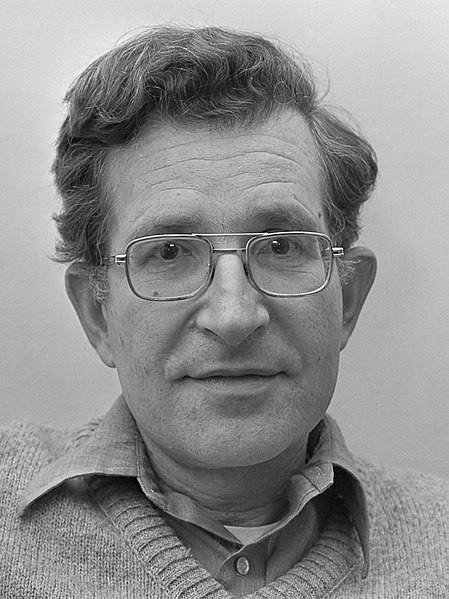
\includegraphics[]{Chomsky1977.jpg}
\end{subfigure}
\begin{subfigure}{.6\textwidth}
\begin{tabular}{lcrl}
Type-0\!\!\!\!\!\!&(무제약)  &\!\!\!\!\!\!문법:& $\alpha\to\gamma$
\\    \!\!\!\!\!\!&$^{\text{unrestricted}}$& \\
Type-1\!\!\!\!\!\!&(문맥의존)&\!\!\!\!\!\!문법:& $\alpha A\beta\to\alpha\gamma\beta$
\\    \!\!\!\!\!\!&$^{\text{context-sensitive}}$& \\
Type-2\!\!\!\!\!\!&(문맥자유)&\!\!\!\!\!\!문법:& $A\to \gamma$
\\    \!\!\!\!\!\!&$^{\text{context-free}}$& \\
Type-3\!\!\!\!\!\!&(정규)    &\!\!\!\!\!\!문법:& $A\to a$, $A\to bB$
\\    \!\!\!\!\!\!&$^{\text{regular}}$&
\end{tabular}
\begin{center}
\quad$a,b\in \Sigma$,\quad$A,B\in N$,\quad$\alpha,\beta,\gamma\in(\Sigma\cup N)^{*}$
\end{center}
\end{subfigure}
\caption{촘스키의 1977년 사진 및 촘스키 계층별 문법의 생성규칙 형태
         \label{fig:ChomskyHierarchyGrammar}\\
         {\scriptsize(사진 출처: 위키미디어 공용)} }
\end{figure}
\noindent
촘스키는 문법에서 생성규칙의 형태를 얼마나 제약하는가를 기준으로 형식문법을
네 계층으로 분류하였는데\cite{Chomsky56}, 이를
\index{촘스키 계층|see{Chomsky hierarchy}}%
\index{Chomsky hierarchy|see{촘스키 계층}}%
촘스키 계층(Chomsky hierarchy)이라고
한다 (그림\;\ref{fig:ChomskyHierarchyGrammar}).
촘스키 계층의 문법은 Type-0부터 Type-3까지의 번호가 들어간 이름으로도,
또 그 특성을 드러낸 이름으로도 불린다. 이를테면 ``Type-3 문법''과
``정규문법''(regular grammar)은 같은 뜻의 용어이다. 번호가 작을수록
제약이 적기 때문에 더 다양한 형태의 문법 규칙이 허용되며 번호가 클수록
더 제한된 형태의 문법 규칙만이 허용된다. 따라서 Type-0이 생성문법의
가능한 모든 규칙이 허용되는 가장 큰 문법의 범주이며, Type-1은 Type-0의 일부분,
Type-2는 Type-1의 일부분, Type-3은 Type-2의 일부분이다. 즉,
모든 정규문법은 문맥자유문법이기도 하고, 모든 문맥자유문법은 문맥의존문법이기도 하며,
모든 문맥의존문법은 무제약문법이기도 하다.

\index{무제약문법|see{unrestricted grammar}}%
\index{unrestricted grammar|see{무제약문법}}%
\index{촘스키 계층!무제약문법}%
\index{Chomsky hierarchy!unrestricted grammar}%
\index{재귀열거언어|see{recursively enumerable language}}%
\index{recursively enumerable language|see{재귀열거언어}}%
\index{촘스키 계층!재귀열거언어}%
\index{Chomsky hierarchy!recursively enumerable language}%
무제약문법(unrestricted grammar)은 생성규칙의 형태에 아무런 제약 없이
화살표의 왼쪽과 오른쪽에 아무런 확장된 문자열이나 다 쓸 수 있다. 예를 들면
$bABa \to aBbaAb$ 같은 복잡한 규칙도 허용된다. 그러니까 문자열의 생성 과정에서
임의 개수의 단말과 비단말을 또 다른 임의 개수의 단말과 비단말로 바꿔나갈 수 있다.
무제약문법으로 표현가능한 언어의 범주를
`재귀열거언어'(recursively enumerable language)라 한다.

\index{문맥의존문법|see{context-sensitive grammar}}%
\index{context-sensitive grammar|see{문맥의존문법}}%
\index{촘스키 계층!문맥의존문법}%
\index{Chomsky hierarchy!context-sensitive grammar}%
문맥의존문법(context-sensitive grammar, CSG)은 화살표 왼쪽에서 비단말 기호 하나만을
치환하며 생성해 나가는 규칙만 허용한다. $\alpha A\beta\to\alpha\gamma\beta$ 형태의
규칙은 $\alpha$와 $\beta$ 사이에 나타나는 비단말 기호 $A$를 $\gamma$로 치환하라는 뜻이다.
이 규칙으로는 $A$의 앞과 뒤에 $\alpha$와 $\beta$가 나타나지 않으면
$A$를 $\gamma$로 치환할 수 없다. 문맥의존문법으로 표현가능한 언어의 범주를
`문맥의존언어'(context-sensitive language, CSL)라 한다.

\index{문맥자유문법|see{context-free grammar}}%
\index{context-free grammar|see{문맥자유문법}}%
\index{촘스키 계층!문맥자유문법}%
\index{Chomsky hierarchy!context-free grammar}%
문맥자유문법(context-free grammar, CFG)은 문맥의존문법의 생성규칙 형태인
$\alpha A\beta\to\alpha\gamma\beta$에서 $\alpha$와 $\beta$ 모두 길이 0인
빈 문자열이라는 (즉, $\alpha=\beta=\varepsilon$) 추가적인 제약이 있는 셈이다.
즉, 문맥자유문법 생성규칙 $A\to\gamma$에 따르면 $A$의 주변에 무엇이 있든 없든
관계없이 $A$를 어디서나 $\gamma$로 치환할 수 있다. 문맥자유문법으로 표현가능한
언어의 범주를 `문맥자유언어'(context-free language, CFL)라 한다.

\index{정규문법|see{regular grammar}}%
\index{regular grammar|see{정규문법}}%
\index{촘스키 계층!정규문법}%
\index{Chomsky hierarchy!regular grammar}%
정규문법(regular grammar)은 문맥자유문법의 생성규칙 형태인 $A\to\gamma$에서
화살표 오른쪽 $\gamma$의 형태를 단말 기호 하나($a$) 또는
단말과 비단말 기호 하나씩($bB$)으로 추가적으로 제한한 것이다.
정규문법으로 표현가능한 언어의 범주는 `정규언어'(regular language)이다. 
참고로 정규언어는 생성규칙의 형태로 표기하기에는 너무 간단한 언어라서
정규문법 대신에 `정규식'(regular expression)으로 표현하여 활용하는 경우가 많다.
정규식에 대해서는 다음 장에서 프로그래밍언어의 어휘분석을 다루면서 설명하겠다.

\begin{figure}[b]\centering
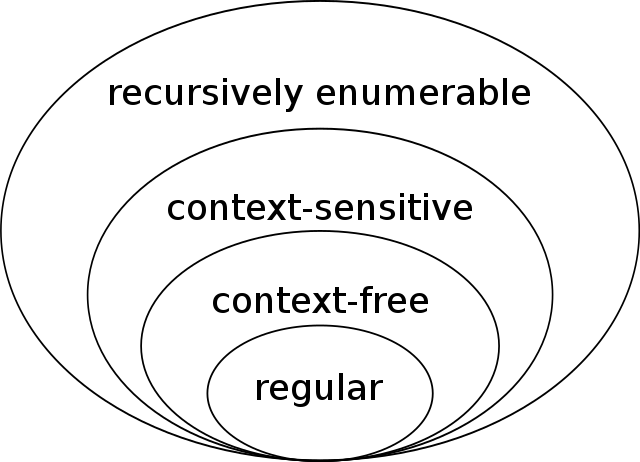
\includegraphics[scale=0.5]{ChomskyHierarchy.png}
\caption{촘스키 계층의 문법에 대응되는 언어 범주의 포함관계
         \label{fig:ChomskyHierarchyLang}\\
         {\scriptsize(이미지 출처: 위키미디어 공용)} }
\end{figure}

정규언어는 여러 번 반복되는 구조가 나타나는 포함할 수 있지만
문자열의 특정 지점까지 몇 번이나 반복했는지 그 횟수를 기억해
이후의 문자열이 어떤 내용이 되어야 언어에 포함시킬지에 판별하는 데
영향을 미칠 수 없다는 것이 특징적인 성질이다. 예제로 다루던 언어
$L = \{\, {\txtbullet\txtcircle}
      ,\, {\txtbullet\txtcircle}{\txtbullet\txtcircle}
      ,\, {\txtbullet\txtcircle}{\txtbullet\txtcircle}{\txtbullet\txtcircle}
      ,\, \ldots
   \,\}$는 $\txtbullet\txtcircle$이 1회 이상 반복되어 나타나는
모든 문자열로 이루어져 있는 정규언어이다.
하지만 언어 $L_p = \{\txtbullet^n\txtcircle^n \mid n>0\}$는
정규언어가 아니다. 왜냐하면 백돌이 나타나기 전까지 흑돌의 개수를
기억했다 후반부에 나타나는 백돌의 개수와 맞춰봐야 $L_p$에 포함되는
문자열인지 구분할 수 있기 때문이다. 그래서 정규언어로는 괄호의 쌍을
맞추도록 처리하는 것이 불가능하다. 괄호가 이전까지 몇 번 열렸는지
기억하고 있어야 그에 쌍을 맞춰 괄호를 닫을 수 있는데 정규언어는
그보다 더 단순히 횟수를 기억하지 못하는 반복 구조만을 다룰 수 있다.

정규언어의 범주를 넘어선 문맥자유언어의 범주에서는 괄호를 맞출 수 있다.
문맥자유문법 $G_p =
   \left\langle\, \{\txtbullet,\txtcircle\},\, \{S,A\},\, S,\,
                  \{\,S\to\txtbullet\,\txtcircle,\,S\to\txtbullet\,S\,\txtcircle\,\}
\,\right\rangle$로 바로 위에서 정규언어가 아닌 예로 들었던 언어 $L_p$를 표현할 수 있다.
$L_p$의 문자열인 \txtbullet\txtbullet\txtcircle\txtcircle를 $G_p$에 따라
다음과 같이 생성할 수 있다.
\begin{center}
\begin{forest}
for tree={fit=tight, l sep-=.5em, inner sep=0, l=0}
[$S$ [\txtbullet,tier=word]
     [$S$ [\txtbullet,tier=word] [\txtcircle,tier=word]]
     [\txtcircle,tier=word]
]
\end{forest}
\end{center}
이렇듯 문맥자유언어의 범주에서는 쌍을 맞춰가며 개수를 비교해 언어에 포함되는
문자열인지 판단할 수 있다. 그러나 그보다 더 복잡한 구조에서 개수를 비교해
문자열이 언어에 포함되는지 따지는 것은 불가능하다. 서로 다른 세 문자가 모두
같은 개수만큼 차례로 나타나는 $\{a^nb^nc^n\mid n>0\}$은 문맥자유언어가 아닌 예로
잘 알려진 언어이다. 나란히 있는 $a$와 $b$끼리 또는 $b$와 $c$끼리 쌍을 맞춰가거나
아니면 가운데 $b$를 남겨놓고 $a$와 $c$끼리 쌍을 맞춰가며 개수를 비교할 수는 있지만,
동시에 세 부분의 개수를 맞는지 따지는 것은 문맥자유언어의 범주에서 불가능하다.
참고로 $\{a^nb^nc^n\mid n>0\}$는 문맥의존문법으로 표현가능한 문맥의존언어의 범주에 속한다.


\section*{요점정리}
\begin{itemize}[itemsep=0pt]
    \item 형식언어이론에서 언어란 문자열의 집합으로 정의된다.
    \item 형식언어의 문법 $G=\langle\Sigma,N,S,R\rangle$은
    최종 문자열을 구성하는 단말 기호의 집합($\Sigma$),
    생성 도중에만 나타나는 비단말 기호의 집합($N$),
    생성 과정의 처음을 나타내는 시작 기호($S$),
    생성규칙의 집합($R$)의 네 요소로 정의된다.
    \item 문법의 핵심적인 요소인 $\alpha\to\beta$의 형태의 생성규칙에 따라
    화살표 왼쪽에 나타나는 확장된 문자열($\alpha$)을 오른쪽에 나타나는
    확장된 문자열($\beta$)로 치환해 나가는 과정을 단말 기호로만 이루어진
    문자열이 생성되기까지 반복한다.
    \item 문법 $G$가 언어 $L$을 표현한다는 것은 문법에 따라 생성 가능한 모든
    문자열의 집합이 주어진 언어와 일치, 즉 $\mathcal{L}(G) = L$임을 뜻한다.
    일반적으로 하나의 언어를 표현하는 문법은 여러 가지로 작성 가능하다.
    \item 문자열 유도(derivation) 과정의 순차적 나열 대신
    문법나무(syntax tree)의 형태로 표현하면 중복된 표기가 줄어들어
    한눈에 알아보기 좋다.
    \item 같은 문자열을 생성하는 서로 다른 문법나무가 여럿인 경우가
    있다면 모호한 문법이다.
    \item 언어를 표현하는 문법이 모두 모호한 경우, 즉 아무리 신경써서
    문법을 작성해도 모호하지 않은 문법으로는 표현할 수 없는 경우에
    (태생적으로) 모호한 언어라고 한다.
    \item 촘스키는 생성규칙 형태의 제약 정도에 따라 문법을 네 계층으로 분류하였으며
    (정규$\,\subset\,$문맥자유$\,\subset\,$문맥의존$\,\subset\,$무제약),
    그에 대응되는 언어의 범주도 네 계층을 이룬다
    (정규$\,\subset\,$문맥자유$\,\subset\,$문맥의존$\,\subset\,$재귀열거).
    \item 정규언어의 범주에서는 횟수를 기억하지 않는 한에서 반복된 구조를
    판별할 수 있으며, 문맥자유언어의 범주에서는 여닫는 괄호의 개수를 맞추는
    것과 같이 쌍을 맞춰가는 반복된 구조를 판별할 수 있다.
\end{itemize}

\section*{연습문제}
\begin{enumerate}
\item 다음 문맥자유언어에 대한 형식문법을 작성해 보라.\\
$\displaystyle
 \left\{ \mathtt{d}\mathtt{s}^n\mathtt{o}\mathtt{z}^n\mathtt{b}
           \mid
           n\ge0 \right\}
 =
 \left\{ \mathtt{dob}
       , \mathtt{dsozb}
       , \mathtt{dssozzb}
       , \mathtt{dsssozzzb}
       , \ldots \right\}$

\item 다음 문맥자유언어에 대한 형식문법을 작성해 보라.\\
$\displaystyle
 \left\{ \mathtt{w}^n\mathtt{o}\mathtt{v}^{2n}
           \mid
           n\ge1 \right\}
 =
 \left\{ \mathtt{wov}
       , \mathtt{wwovvvv}
       , \mathtt{wwwovvvvvv}
       , \ldots \right\}$
\end{enumerate}

\chapter[프로그래밍언어의 문법구조(Syntax)]{프로그래밍언어의\\문법구조(Syntax)}
프로그래밍언어의 설명서는 어휘구조(lexical structure)라는 항목이
등장하며, 어휘가 모여 어떻게 구문구조(syntax)를 이루는지에 대한
설명도 이어진다. 그렇게 `-구조'를 붙여 우리말로 옮기는 것과 일관되게
프로그래밍언어의 겉모양과 속뜻에 해당하는 용어를
\index{문법구조|see{syntax}}%
\index{syntax|see{문법구조}}%
문법구조(syntax)와
\index{의미구조|see{semantics}}%
\index{semantics|see{의미구조}}%
의미구조(semantics)로 옮기기도 한다. 이 장에서는 프로그래밍언어의
문법구조와 관련된 개념과 용어를 소개한다.

어휘구조(lexical structure)와 나란히 쓰이는 구문구조(syntax)와
의미구조(semantics)와 나란히 쓰이는 문법구조(syntax)의
syntax는 같은 영어 단어라도 다른 맥락에서 쓰이는 조금 다른 개념이다.
두 개념을 함께 다룰 때는 그 차이가 분명히 드러나도록
전자를 ``구체적 문법''(concrete syntax) 후자를
``추상(또는 요약) 문법''이라고 구분하여 부르기도 한다.
이 장에서 설명할 내용을 통해 이렇게 비슷하지만 다른 맥락에서
조금씩 다른 개념으로 쓰이는 용어를 구별하여 이해하는 데 도움이
되기를 바란다.

\newpage

\section{어휘 및 구문 분석}
\label{sec:LexParse}
프로그래밍언어의 설명서\cite{Swift5Ref,CSharp6Draft,JavaSE8spec,Haskell2010}에서
흔히
\index{어휘구조|see{lexical structure}}%
\index{lexical structure|see{여휘구조}}%
어휘구조(lexical structure)라는 항목 하에 글자들이 모여 어떤 종류의
어휘를 이루는지, 그러니까 리터럴(literal), 식별자(identifier), 연산자(operator),
키워드/예약어(keyword/reserved word), 주석(comment) 등이 되는지 설명한다.
\index{구문구조|see{syntax}}%
\index{syntax|see{구문구조}}%
그런 어휘가 모여 어떻게 구문구조(syntax)를 이루는지를 다루는 내용은
어휘구조에 비해 더 복잡하므로 식(expression), 문(statement), 블럭(block) 등의
요소별로 별도의 항목으로 나누어 설명하는 것이 일반적이다.

프로그래밍언어의 소스코드는 일차원적으로 나열된 문자열로 작성되어 있다.
이렇게 한줄로 이어진 문자열로부터
\index{어쉬분석|see{lexical analysis}}%
\index{lexical analysis|see{어휘분석}}%
어휘분석(lexical analysis) 단계를 거치면
하나 혹은 그 이상의 글자들로 이루어진 어휘(lexeme)를 각각 끊어냄으로써
어휘구조를 인식하고, 각각 어떤 종류의 어휘인지 구별된
\index{토큰|see{token}}%
\index{token|see{token}}%
토큰(token)의
나열인 토큰열을 얻는다. 토큰열로부터
\index{문법분석|see{syntax analysis}}%
\index{syntax analysis|see{문법분석}}%
문법분석(syntax analysis) 단계를
거치면 구문구조를 인식하며
\index{구체적문법나무}
\index{concrete syntax tree}
구체적문법나무(concrete syntax tree)를 구성하고,
그 핵심만을 요약한
\index{추상문법나무|see{abstract syntax tree}}%
\index{abstract syntax tree|see{추상문법나무}}%
\index{문법나무!추상문법나무}%
\index{syntax tree!abstract syntax tree}%
\index{AST|see{abstract syntax tree}}%
\index{AST|see{추상문법나무}}%
추상문법나무(abstract syntax tree, AST)를 얻는다.
그림\;\ref{fig:LexParse}에는 뺄셈, 곱셈, 거듭제곱 연산을 포함한
산술식(arithmetic expression)을 예시로 어휘분석 및 구문분석 과정에서
나타나는 네 가지 데이터 구조들인 문자열, 토큰열, 구체적문법나무,
추상문법나무가 한눈에 잘 알아볼 수 있도록 나타나 있다.
그림\;\ref{fig:LexParse}의 각 구조에 대해 예시를 중심으로 조금
더 알아보자.

\begin{figure}\centering
\setlength{\tabcolsep}{.8ex}
\renewcommand{\arraystretch}{1.25}
\begin{subfigure}{.8\textwidth}\ttfamily
\begin{tabular}{| *{25}{m{.8ex}|} }
\hline 
5& &*& &(& & & &1&0& &-& &8&)& &*& &2&\char`^&2& &\char`^& &3\\
\hline
\end{tabular}
\caption{문자열(sequence of characters)\label{sfig:charseq}}
\end{subfigure}
~\\
\hfill
\begin{subfigure}{.65\textwidth}\ttfamily
~\\[1ex]
\fbox{$5$}
\fcolorbox{teal}{teal!20}{*}
\fcolorbox{brown}{brown!20}{(}
\fbox{$10$} \fcolorbox{teal}{teal!20}{-} \fbox{$8$}
\fcolorbox{brown}{brown!20}{)}
\fcolorbox{teal}{teal!20}{*}
\fbox{$2$}
\fcolorbox{teal}{teal!20}{\textbf{\char`^}} \fbox{$2$}
\fcolorbox{teal}{teal!20}{\textbf{\char`^}} \fbox{$3$}
\caption{토큰열(sequence of tokens)\label{sfig:tokseq}}
\end{subfigure}
\\[-7ex]
\qquad
\begin{subfigure}[b]{.4\textwidth}
\begin{forest}
for tree={l sep-=.8em, l-=.8em, inner sep=0, l=0}
[$E$ [$T$, for current={s sep=+2em}, for children={s sep+=1em}
  [$T$ 
       [$F$ [$A$ [$5$]]]
       [$*$]
       [$F$ [$A$, for current={s sep+=1em}
         [$($]
         [$E$
           [$E$ [$T$ [$F$ [$A$ [$10$]]]]]
           [$-$]
           [$T$ [$F$ [$A$ [$8$]]]]
         ]
         [$)$]
       ]]
  ]
  [$\phantom{a}\quad*\quad\phantom{a}$]
  [$F$
    [$A$ [$2$]]
    [\textbf{\char`^}]
    [$F$ [$F$ [$A$ [$2$]]] [\textbf{\char`^}] [$A$ [$3$]]]
  ]
]]
\end{forest}
\subcaption{구체적문법나무\\(concrete syntax tree)\label{sfig:CST}}
\end{subfigure}
\hfill
\begin{subfigure}[b]{.4\textwidth}\centering\ttfamily
\begin{forest}
for tree={inner sep=0, l sep+=1em, l=0}
[*,circle,draw,for current={s sep+=1em}
   [*,circle,draw,for current={s sep+=1em}
      [$5$]
      [-,circle,draw [$10$] [$8$]]
   ]
   [\textbf{\char`^},circle,draw,for current={s sep+=1em}
      [$2$]
      [\textbf{\char`^},circle,draw [$2$] [$3$]]
   ]
]
\end{forest}
\subcaption{추상문법나무(요약문법나무)\\(abstract syntax tree)\label{sfig:AST}}
\end{subfigure}
\caption{\lstinline[columns=flexible
                   ,keepspaces=true
                   ,showspaces=true]|"5 * ( {} {} 10 - 8) * 2^2 ^ 3"|에 대한
         어휘분석 과정({\scriptsize(a)$\to$(b)})과 
         구문분석 과정({\scriptsize(b)$\to$(c)$\to$(d)})에 나타나는 데이터 구조들
         \label{fig:LexParse}}
\end{figure}

그림\;\ref{sfig:charseq}는 문자열
\lstinline[columns=flexible,
                   ,keepspaces=true
                   ,showspaces=true]|"5 * (   10 - 8) * 2^2 ^ 3"|를
이루는 각각의 글자(character)를 일차원적인 공간에 차례대로 배치하고 있다.
(참고로, 여기서는 공백 문자임을 강조하기 위해 빈칸으로 나타내는 대신
\lstinline[columns=flexible
                   ,keepspaces=true
                   ,showspaces=true]| |로 표시하였다.)
이 문자열은 0부터 9까지 십진수 숫자(digit); 뺄셈, 곱셈, 거듭제곱 등의
산술 연산을 나타내는 기호; 열고 닫는 괄호 기호; 그리고 공백 문자로
이루어져 있다. 들여쓰기로 블럭을 구분하거나 공백 없이 붙여쓰면 하나의
어휘로 인식되는 경우를 제외하면, 사람의 눈에 알아보기 좋은 소스코드가
되도록 공백 문자를 적당히 추가하더라도 내용에는 실제적인 영향을
미치지 못하는 경우가 대부분이다. 즉,
\lstinline[columns=flexible
                   ,keepspaces=true
                   ,showspaces=true]|"5*(10-8)*2^2^3"|처럼
공백을 제외한 문자열도 똑같은 수식을 표현하게 된다.

그림\;\ref{sfig:tokseq}는 앞서 언급한 문자열의 어휘분석 결과로 나온
토큰열을 나타낸다. 5나 \texttt{*}와 같이 하나의 글자로 된 어휘도 있지만
10과 같이 두 개 이상의 글자가 모여 하나의 어휘를 이루기도 한다.
문자열에서 어휘를 끊어내면서 어휘 사이의 공백 문자는 버린다.
단지 어휘를 끊어낼 뿐만 아니라 어휘의 종류를 구분하여 정리해 놓는데,
이렇게 종류가 구분된 어휘를 토큰(token)이라고 한다.
5, 10, 6 등은 정수 리터럴(integer literal),
\texttt{*}, \texttt{-}, \texttt{\textbf{\char`^}} 등은 연산자,
열고 닫는 괄호 등의 토큰으로 구분됨을 색상으로 표시하였다.
결과로 토큰열을 얻으므로 어휘분석을
\index{토큰화|see{tokenization}}%
\index{tokenization|see{토큰화}}%
토큰화(tokenization)라고도 한다.
프로그래밍언어 분야에서는
\index{어휘분석}%
\index{lexical analysis}%
어휘분석(lexical analysis)을 줄여
렉싱(lexing)이라 부르는 경우가 많다. 따라서 어휘분석을 수행하는
프로그램인 어휘분석기(lexical analyzer)를 토크나이저(tokenizer)라고도 하며,
프로그래밍언어의 경우
\index{렉서|see{lexer}}%
\index{lexer|see{렉서}}%
렉서(lexer)라 부르는 경우가 많다.

\index{구문분석}%
\index{syntax analysis}%
구문분석(syntax analysis)은 언어학 및 컴퓨터 관련 분야에서
파싱(parsing)이라고도 한다. 참고로 파싱(parsing)의 어원이 되는 동사
parse는 품사(parts of speech)를 뜻하는 라틴어에서 유래했다\cite{MWdict}.
즉, parse란 문장을 구성하는 각 부분이 문법적으로 어떤 부류에
속하는지 인식해 문장의 구조를 분석한다는 뜻으로 이해할 수 있다.
구문분석을 수행하는 프로그램인 구문분석기(syntax analyzer)를
컴퓨터 관련 분야에서
\index{파서|see{parser}}%
\index{parser|see{파서}}%
파서(parser)라 부르는 경우가 많다.
프로그래밍언어의 파서는 토큰열(그림\;\ref{sfig:tokseq})로부터
\index{구체적문법나무}%
\index{concrete syntax tree}%
구체적문법나무(그림\;\ref{sfig:CST})를 구성하고 이를 요약한
\index{추상문법나무}%
\index{abstract syntax tree}%
추상문법나무(그림\;\ref{sfig:AST})를 만들어낸다. `추상문법나무'는
프로그래밍언어의 의미를 다루기 위한 핵심적 부분만을 요약하고 있으므로
\index{문법나무!요약문법나무}%
\index{syntax tree!abstract syntax tree}%
\index{요약문법나무|see{abstract syntax tree}}%
\index{abstract syntax tree|see{요약문법나무}}%
\index{AST|see{요약문법나무}}%
`요약문법나무'로도 옮긴다. 또한 구체적문법나무(concrete syntax tree)와
요약문법나무(abstract syntax tree)대신 파스나무(parse tree)와
문법나무(syntax tree)로도 일컫는다. 파서(parser)의 최종 결과물은
파스나무(즉, 구체적문법나무)가 아니라 문법나무(즉, 요약문법나무)다.

정리하면, 프로그래밍언어의 문법(syntax)을 두 단계로 구분해 생각할 수 있다.
첫째는 토큰열로부터 구체적문법나무를 구성하기 위한
\index{문법!구체적문법}%
\index{syntax!concrete syntax}%
\index{구체적문법|see{concrete syntax}}%
\index{concrete syntax|see{구체적문법}}%
구체적문법(concrete syntax), 둘째는 요약문법나무의 구조를
나타내는
\index{문법!요약문법}%
\index{syntax!abstract syntax}%
\index{요약문법|see{concrete syntax}}%
\index{추상문법|see{concrete syntax}}%
\index{concrete syntax|see{요약문법}}%
\index{concrete syntax|see{추상문법}}%
요약문법(abstract syntax)이다. 물론 요약문법을
추상문법이라고도 옮긴다. 이제부터 이 책에서는 `추상-'보다는 `요약-'이 붙은
용어를 사용하기로 한다. 이어지는 절(\ref{sec:GrammarNotation}절)에서는
구체적문법과 요약문법의 표기방법에 대해 대해 먼저 알아보고,
그 다음 절(\ref{sec:regex}절)에서 어휘분석에 활용되는 정규식에
대해 알아보기로 하자.

\section{문법의 표기}
\label{sec:GrammarNotation}
앞절에서 정리한 바와 같이, 프로그래밍언어의 구체적문법은 일차원적 구조인
토큰열로부터 구체적문법나무를 하나로 결정할 수 있어야 하므로 모호함 없는
(unambiguous) 문맥자유문법으로 정의되어야 한다. 참고로 문맥자유문법에서
모호함의 개념에 대해서는 \ref{sec:ambiguous}절에서 다룬 바 있다.
프로그래밍언어의 문법에서 모호함을 해소해야 하는 대표적인 요소로
연산자(operator)의 우선순위(precedence)와 결합성(associativity)을 들 수 있다.
우선순위는 서로 다른 연산자들 사이에 어느 연산자가 우선하는지를 말한다.
보통 곱셈과 나눗셈 연산이 덧셈과 뺄셈 연산보다 우선순위가 높으므로
$8\mathop{\texttt{-}} 3\mathop{\texttt{*}}2 $는
$8\mathop{\texttt{-}}(3\mathop{\texttt{*}}2)$와 같은 의미다.
결합성은 같은 연산자가 연달아 사용하는 것이 가능한지 그리고
가능하다면 어떤 방향으로 결합이 우선하는지를 말한다.
보통 좌결합(left-associative)인 뺄셈의 경우
$ 8\mathop{\texttt{-}}3 \mathop{\texttt{-}}2$는
$(8\mathop{\texttt{-}}3)\mathop{\texttt{-}}2$와 같고
우결합(right-associative)인 거듭제곱의 경우
$2\mathop{\texttt{\char`^}} 2\mathop{\texttt{\char`^}}3 $는
$2\mathop{\texttt{\char`^}}(2\mathop{\texttt{\char`^}}3)$와 같은 의미다.
그리고 기본적인 연산자 우선순위 및 결합성과 달리 순서를 명시적으로
강제하기 위한 괄호(parenthesis) 또한 구체적문법에 포함되곤 한다.
요약문법은 이미 구체적문법으로 모호함 없이 분석된 바를 요약한 구조만을 다루므로,
일차원적 구조에서 고려해야 하는 연산자 우선순위나 결합성을 따질 필요가 없으며
괄호와 같이 우선순위를 명시적으로 강제하는 요소도 불필요하다.
이제 사칙연산(\texttt{+}, \texttt{-}, \texttt{*}, \texttt{/})과
거듭제곱(\texttt{\char`^})을 포함한 산술식에 대한 구체적문법과
요약문법의 표기에 대해 알아보자.

그림\;\ref{fig:BNF}는 똑같은 산술식의 구체적문법(concrete syntax)을
나타내는 형식문법의 생성규칙과 BNF 표현을 나란히 비교하고 있다.
참고로 화살표 왼쪽이 같은 비단말인 생성규칙끼리 묶어 간략하게 표기하기도 한다.
예를 들면 세 개의 규칙
$E \to E ~\texttt{+}~ T$, $E \to E ~\texttt{-}~ T$, $E \to T$를
한꺼번에 $E \to E\;\texttt{+}\;T \mid E\;\texttt{-}\;T \mid T$로
묶어 표기한다. 그림\;\ref{fig:BNF}의 생성규칙도 이렇게 묶어 표기한 형태로
그 바로 옆에 나란히 나타난 BNF 표현의 구조와 일치한다.
즉, 비단말 $E$, $T$, $F$, $A$, $Z$를 각각 \texttt{<expr>},
\texttt{<term>}, \texttt{<factor>}, \texttt{<atom>}, \texttt{<integer>}에 대응시키고, 단말은
쌍따옴표(\texttt{"})로 둘러싸고, $\to$를 \texttt{::=}로
바꾸기만 하면, 생성규칙을 BNF로 옮길 수 있다. 형식문법의 생성규칙은
마치 수학에서 수식과 같이 주로 이론적 논의를 위한 간결함을 우선시하여
비단말은 대문자 단말은 소문자 한 글자씩만으로 표시한다.
프로그래밍언어 분야에 선구적 업적을 남긴
두 컴퓨터 과학자(그림\;\ref{fig:BackusNaur})의 이름을 딴
\index{배커스--나우르 형식|see{Backus--Naur Form}}%
\index{Backus--Naur Form|see{배커스--나우르 형식}}%
\index{BNF|see{Backus--Naur Form}}%
\index{BNF|see{배커스--나우르 형식}}%
배커스--나우르 형식(Backus--Naur Form, BNF)은 프로그래밍언어의
구체적문법을 정의하는 등의 실용적인 활용을 염두에 두고 만들어졌다.
BNF는 알아보기 쉬운 단어로 비단말을 표현하거나 여러 글자로 된 단말의
표현도 가능한, 실용적 편의성을 고려된 문맥자유문법의 표기 방식이다.

\begin{figure}\centering
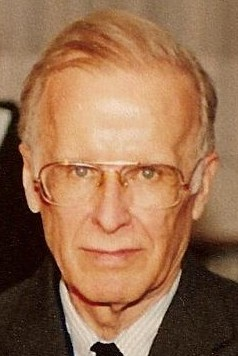
\includegraphics[scale=0.25]{JohnBackus.jpg}
\qquad\qquad\qquad
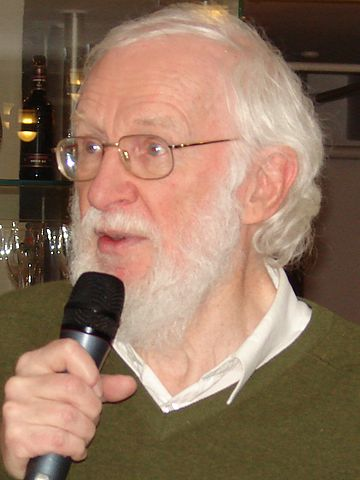
\includegraphics[scale=0.21]{PeterNaur.jpg}
\caption{Fortran 언어의 창시자인 John Backus(1999년 사진, 좌)와\\
         ALGOL 60 언어 개발을 주도한 Peter Naur(2008년 사진, 우)\\
         {\scriptsize(사진 출처: 위키미디어 공용)}\label{fig:BackusNaur}}
\end{figure}
\begin{figure}[H]\vspace*{-4ex}
\hfill
\begin{subfigure}[b]{.2\linewidth}\addtolength{\jot}{-.3em}
\begin{align*}
E \to~& E ~\texttt{+}~ T \\
 \mid~& E ~\texttt{-}~ T \\
 \mid~& T \\
T \to~& T ~\texttt{*}~ F \\
 \mid~& T ~\texttt{/}~ F \\
 \mid~& F \\
F \to~& A ~\texttt{\char`^}~ F \\
 \mid~& A \\
A \to~& Z \\
 \mid~& \texttt{(}~ E ~\texttt{)}
\end{align*}
~\vspace*{-2.8ex}
\end{subfigure}
\qquad\qquad
\begin{subfigure}[b]{.6\linewidth}
\begin{lstlisting}
<expr>   ::= <expr> "+" <term>
           | <expr> "-" <term>
           | <term>
<term>   ::= <term> "*" <factor>
           | <term> "/" <factor>
           | <factor>
<factor> ::= <atom> "^" <factor>
           | <atom>
<atom>   ::= <integer>
           | "(" <expr> ")"
\end{lstlisting}
\end{subfigure}
\caption{사칙연산과 거듭제곱을 포함한 산술식의 생성규칙과 BNF 비교\\
         {\small(위에서 $Z$와 \texttt{<integer>}는 정수 리터럴을 대표하는 비단말)}
         \label{fig:BNF}}
\end{figure}
\begin{figure}[H]\vspace*{-4ex}
\begin{subfigure}[b]{0.3\textwidth}
\begin{lstlisting}[language=Haskell,basicstyle=\linespread{1.1}\ttfamily]
data E = Add E E
       | Sub E E
       | Mul E E
       | Div E E
       | Exp E E
       | Lit Integer
\end{lstlisting}
~\vspace{-3.3ex}
\subcaption{Haskell 데이터 타입\label{sfig:HaskellADT}}
\end{subfigure}
\hfill
\begin{subfigure}[b]{0.3\textwidth}\addtolength{\jot}{-.2em}
\begin{align*}
E  \to ~& E ~\texttt{+}~ E
\\ \mid~& E ~\texttt{-}~ E
\\ \mid~& E ~\texttt{*}~ E
\\ \mid~& E ~\texttt{/}~ E
\\ \mid~& E ~\texttt{\char`^}~ E
\\ \mid~& Z
\end{align*}
~\vspace{-4ex}
\subcaption{형식문법의 생성규칙\label{sfig:GrammarAS}}
\end{subfigure}
\hfill
\begin{subfigure}[b]{0.3\textwidth}\addtolength{\jot}{-.2em}
\begin{align*}
n\in \mathbb{Z} \qquad\;& \\
e\in E ~
   ::= ~& e ~\texttt{+}~ e
\\ \mid~& e ~\texttt{-}~ e
\\ \mid~& e ~\texttt{*}~ e
\\ \mid~& e ~\texttt{/}~ e
\\ \mid~& e ~\texttt{\char`^}~ e
\\ \mid~& n_{\phantom{g}}
\end{align*}
~\vspace{-4ex}
\subcaption{BNF와 수학적 기호\label{sfig:MathAS}}
\end{subfigure}
\caption{요약문법(abstract syntax)의 여러 가지 표현 방식
         \label{fig:AbsSyn}}
\end{figure}

\index{구체적문법}
\index{concrete syntax}
산술식의 구체적문법(그림\;\ref{fig:BNF})에서 주목할 점은 이 절의
앞부분에서 언급한 연산자의 우선순위와 결합성이 드러난다는 것이다.
먼저 BNF 표현을 기준으로 연산자 우선순위를 어떻게 표현되어 있는지 알아보자.
가장 아래쪽에 가장 강력하게 묶이는 식의 구성요소에 대한 규칙에서부터
위로 갈수록 느슨하게 묶이는 식의 구성요소에 대한 규칙이 나타난다.
가장 강하게 묶인 요소인 \texttt{<atom>}은
다른 구문 요소로 쪼갤 수 없는 정수 리터럴(\texttt{<integer>})이거나
강제로 괄호로 묶어놓은 식(\texttt{"(" <expr> ")"})으로 이루어진다.
\texttt{<factor>}는 \texttt{<atom>}을 포함하는 거듭제곱식,
\texttt{<term>}은 \texttt{<factor>}를 포함하는 곱셈/나눗셈식,
\texttt{<expr>}은 \texttt{<term>}을 포함하는 덧셈/뺄셈식으로
구성될 수 있다. 따라서 거듭제곱, 곱셈/나눗셈, 덧셈/뺄셈 순으로
강하게 묶이는 연산자 우선순위가 문법규칙에 드러남을 알 수 있다.
이번에는 생성규칙을 기준으로 연산자 결합성이 어떻게 드러나 있는지 알아보자.
$E \to E ~\texttt{+}~ T \mid  E ~\texttt{-}~ T \mid \cdots$를 보면
비단말 $E$를 구성하는 덧셈/뺄셈식에서 연산자의 왼쪽에 $E$가 재귀적으로
나타나므로 $E$는 덧셈/뺄셈 연산자는 좌결합임이 문법규칙에 드러난다.
마찬가지로 곱셈/나눗셈 연산자도 좌결합임이 드러난다.
반면 $F \to~ A ~\texttt{\char`^}~ F \mid \cdots$를 보면 거듭제곱식에서
연산자의 오른쪽에 $F$가 재귀적으로 나타나므로 거듭제곱 연산자는
우결합임이 문법규칙에 드러난다.

그림\;\ref{fig:AbsSyn}은 사칙연산과 거듭제곱을 포함한 산술식의
\index{요약문법}
\index{abstract syntax}
요약문법 표현 세 가지를 나란히 비교하고 있다. 요약문법은 실제
프로그래밍언어의 구현에 활용하기 위한 용도도 있으므로 이를
프로그램에서 활용할 수 있는 데이터 구조로 정의한다. 특히
하스켈(Haskell)처럼 대수적 데이터 타입(algebraic data type)을
지원하는 함수형 언어에서는 추상문법과 같은 나무구조를 재귀적인
데이터 타입으로 자연스럽게 정의할 수 있다.
그림\;\ref{sfig:HaskellADT}의 하스켈 데이터 타입 \texttt{E}는
생성규칙 형태로 표현한 그림\;\ref{sfig:GrammarAS}의 $E$와
사실상 동일한 구조이다. 생성규칙에서 두 피연산자 사이에 오는
중위 표기의 \texttt{+}, \texttt{-}, \texttt{*}, \texttt{/},
\texttt{\char`^} 연산자는 하스켈 데이터 타입 정의에서
맨 앞에 오는 전위 표기의 \texttt{Add}, \texttt{Sub}, \texttt{Mul},
\texttt{Div}, \texttt{Exp}에 대응된다. 이는 어떤 종류의 식인지
구분하는 머리표와 같다. 정수를 대표하는 비단말 $Z$는 하스켈의
정수 타입인 \texttt{Integer}에 대응되는데, 다른 연산으로 구성된 식과
명확히 구별하고자 정수 단독으로 이루어진 식도 머리표 \texttt{Lit}을
붙여 정의한다. 가장 오른쪽의 그림\;\ref{sfig:MathAS}는 BNF와 같은
$::=$ 기호 및 수학의 집합 관련 기호 등을 활용한 추상문법 표현으로,
프로그래밍언어를 이론적으로 다루는 논문\cite{Milner78,tal-toplas99}이나
학술서적\cite{Winskel93,Mitchell96fpl}에서 통용되는 방식이다. 앞으로
이 책에서도 요약문법을 표기할 때 이와 같은 방식으로 나타낼 것이다.

참고로 그림\;\ref{sfig:GrammarAS}의 표현은 형식문법 생성규칙의
형태만을 빌렸을 뿐 엄밀한 의미에서는 형식언어이론에서 말하는
형식문법이라 볼 수 없다. 왜냐하면 형식언어이론에서는 문법의
대상이 되는 언어를 기호의 일차원적 나열인 문자열의 집합으로
정의하는데, 요약문법은 애초부터 요약문법나무(AST)만을 대상으로
할 뿐 일차원적 구조를 직접 처리할 수 없는 문법구조이기 때문이다.

\section{정규식}
\label{sec:regex}
정규언어는 생성규칙 형태의 정규문법보다는
\index{정규식|see{regular expression}}%
\index{regular expression|see{정규식}}%
정규식(regular expression)으로 표현하는 것이
일반적이다. 왜냐하면 정규언어를 활용하며 구체적문법나무나 요약문법나무를
얻고자 하는 경우는 드물기 때문이다. 프로그래밍언어의 어휘분석 단계에서
인식한 어휘 혹은 토큰은 그 다음 구문분석 단계에서 더 이상 쪼개지지 않는
원자적인 기호로 취급된다. 어휘분석 이후로는 어휘나 토큰을 더 작은 단위로
나누거나 내부의 구조를 따질 일이 사실상 없다. 이런 어휘분석이나 문자열의
검색 및 입력 형식 확인 등 대부분의 정규언어 활용 사례에 적합한 표현 방식이
바로 정규식이다.

\begin{figure}[b]\vspace*{-2ex}
\begin{align*}
\text{문법구조(syntax)\hspace{-5ex}} & &~&
&\text{의미구조(semantics)\hspace{-7ex}} & \qquad\qquad\qquad
\text{\makebox[0pt][l]{%
\raisebox{-.92\totalheight}[0pt][0pt]{%
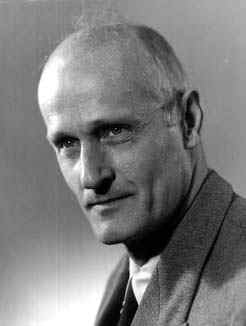
\includegraphics[scale=.25]{Kleene.jpg}}}%
} \\
a \in \Sigma \qquad & &~&
& \llbracket\;\cdot\;\rrbracket ~:~& \mathcal{R}\to 2^{\Sigma^{*}} \\
r \in \mathcal{R}
        ::=\;& \varnothing &\text{\small null}&
& \llbracket\,\varnothing\,\rrbracket \,=\;& \{\,\} \\
       \mid\;& \varepsilon &\text{\small epsilon}&
& \llbracket\,\varepsilon\,\rrbracket \,=\;& \{\varepsilon\} \\
       \mid\;& a &\text{\small symbol}&
& \llbracket\,a\,\rrbracket \,=\;& \{a\} \\
       \mid\;& r_1 \VERT r_2 &\text{\small union}&
& \llbracket\,r_1 \VERT r_2\,\rrbracket \,=\;&
     \llbracket r_1 \rrbracket \cup \llbracket r_2 \rrbracket \\
       \mid\;& r_1\,r_2 &\text{\small concat}&
& \llbracket\,r_1\,r_2\,\rrbracket \,=\;&
     \left\{\,x_1x_2 \mid x_1\in\llbracket r_1\rrbracket,\;
                          x_2\in\llbracket r_2\rrbracket \right\} \\
       \mid\;& r^{*} &\text{\small Kleene star}&
& \llbracket\,r^{*}\,\rrbracket \,=\;&
     \bigcup_{i\in\mathbb{N}} \llbracket\,r^i\,\rrbracket
     \quad\text{\small where}~
     {}_{ \begin{array}{ll} r^0    &\!\!\!\!=\, \varepsilon \\
                            r^{1+n}&\!\!\!\!=\, r\,r^n  \end{array} }
\end{align*}
\vspace*{-3ex}
\caption{정규식의 문법구조와 의미구조,
         반복을 나타내는 별표 표기를 도입한
         스티븐 클레이니(Stephan Kleene)
         {\footnotesize(사진 출처 MacTutor)}
         \label{fig:RegexSynSem}}
\end{figure}

앞절에서 이론적인 맥락에서와 실용적인 활용을 염두에 둔 두 가지 형태의
문맥자유언어에 대한 구체적문법의 표기법(그림\;\ref{fig:BNF})을 살펴보았다.
마찬가지로 정규언어에 대한
\index{정규표현식|see{정규식}}
\index{regex|see{regular expression}}
정규(표현)식(regular expression, regex)도
이론적 형태와 실용적 형태가 조금 다르다. 여기서는 이론적인 형태의
정규식을 주로 알아보자. 정규식도 (넓은 의미에서) 일종의 프로그래밍언어이므로
그림\;\ref{fig:RegexSynSem}와 같이 그 문법구조와 의미구조를 정리해 볼 수 있다.
참고로, $X$의 멱집합 $2^X = \{A\mid A\subset X\}$는 $X$의 모든 부분집합의
집합을 나타낸다. 앞서 \ref{sec:GenGrammar}절에서 형식언어를 다루면서
$\Sigma^{*}$란 알파벳을 $\Sigma$로 삼는 가능한 모든 (유한한 길이의)
문자열 전체의 집합을 나타낸다고 소개했다. 그렇다면 그 멱집합
$2^{\Sigma^{*}}$는 $\Sigma$를 알파벳으로 삼는 문자열로 이루어진
가능한 모든 집합, 즉 알파벳이 $\Sigma$인 모든 형식언어의 집합을 나타낸다.
그러므로 그림\;\ref{fig:RegexSynSem}의 지시함수(denotation function) 혹은
의미값함수(semantic evaluation function) $\llbracket\,\cdot\,\rrbracket$는
정규식($\mathcal{R}$)을 언어($2^{\Sigma^{*}}$)에 대응시킴으로써 정규식의
의미구조를 규정한다. 마지막의 클레이니 별표를 제외하면 기본적인 집합 표현
및 합집합 연산을 사용하는 비교적 간단한 정의이다. 다만 조금 의아하게 느낄
수도 있는 점은 같은 기호가 두 가지 역할을 하고 있다는 것이다.
정규식 $\varepsilon,a\in\mathcal{R}$ 역할도 하고
문자열 $\varepsilon,a\in\Sigma^{*}$ 역할도 한다.
이렇게 한 기호에 여러 가지 의미를 과적(overload)하는 것을
오버로딩(overloading)이라고 한다. 프로그래밍언어를 설명할
때 오버로딩을 나름 신선한 개념인 것처럼 소개하기도 하는데
사실 수학에서는 너무나 일상화되어서 그걸 굳이 오버로딩이라는
용어를 써가며 언급하지도 않는다. 수학에서 $+$같은 기호를 얼마나
다양한 의미로 오버로딩하고 있을지 생각해 보라.

그림\;\ref{fig:RegexSynSem}의 문법구조는 추상문법에 해당하며
구체적문법에는 연산자 우선순위 등에 대한 정보가 추가로 제공되어야 한다.
정규식에서 연산자 우선순위는 강하게 묶이는 순서대로
클레이니 별표(Kleene star), 이어붙이기(concatenation), 합집합(union)이며
산술식과 마찬가지로 괄호로 순서를 강제할 수 있다. 예컨대,
$r_1\VERT r_2\,{r_3}^{*}$는 $r_1\VERT(r_2({r_3}^{*}))$와 같은 의미이다.
정규식의 의미구조를 잘 살펴보면 합집합과 이어붙이기 연산에 대한
결합법칙이 성립함을 알 수 있다.
즉, $r_1\VERT(r_2\VERT r_3)$는 $(r_1\VERT r_2)\VERT r_3$와
같고 $r_1(r_2\,r_3)$는 $(r_1\,r_2)r_3$와 같은 뜻이다.
좌결합이든 우결합이든 의미가 같으므로 결합성을 굳이 따질 필요가 없다.
앞서 산술식의 구체적문법을 설명하며 연산자의 우선순위(precedence)와
결합성(associativity)은 다루었지만 연산자가 나타나는 위치(fixity)에
대한 용어는 정리하지 않았다. 여기서 간단히 정리하자면, 피연산자보다
앞(왼쪽)에 오면 전위(prefix) 뒤(오른쪽)에 오면 후위(postfix)이며
피연산자 사이에 오면 중위(infix)라 한다. 클레이니 별표는 추상문법에서는
방금 살펴본 바와 같이 보통 위첨자 표기로 나타내는데, 구체적문법에 따라
정규식을 문자열로 나타내는 경우에는 \verb/(a|b)*/와 같이 후위로
표기하는 것이 일반적이다.

합집합 연산의 항등원은 $\varnothing$이며
(즉, $\varnothing \VERT r \equiv r \equiv r \VERT \varnothing\,$)
이어붙이기 연산의 항등원은 $\varepsilon$이다
(즉, $\varepsilon\,r \equiv r \equiv r\,\varepsilon\,$).
따라서 클레이니 별표 연산의 의미구조에 나타나는 $r^0$를
이어붙이기 연산의 항등원으로 정의하는 것이 자연스럽다.
왜냐하면 $r^n$은 정규식 $r$을 $n$번 이어붙인 정규식이므로
0번 이어붙인다는 것은 다시 말하면 이어붙인 결과가
그대로여야 하는 항등원을 뜻한다. 또한 분배법칙
$r\,(r_1 \VERT r_2) \equiv r\,r_1 \VERT r\,r_2$가 성립하므로
클레이니 스타와 관련된 공식 $r^{*} \equiv \varepsilon\VERT r\,r^{*}$를
아래와 같이 유도할 수 있다. 당연한 이야기지만 짚고 넘어가자면
의미가 같은 정규식을 동치(equivalence) 관계, 즉,
$\llbracket r_1 \rrbracket = \llbracket r_2 \rrbracket$일 때
$r_1 \equiv r_2$로 표기한다.
$\displaystyle
      \llbracket r^{*} \rrbracket
\;=\; \bigcup_{i\in\mathbb{N}}\llbracket r^i \rrbracket
\;=\; \llbracket r^0 \rrbracket \cup
      \llbracket r^1 \rrbracket \cup
      \llbracket r^2 \rrbracket \cup \cdots
\;=\; \llbracket r^0\VERT r^1\VERT r^2\VERT \cdots \rrbracket$이므로,
\vspace*{-1.5ex}
\begin{align*}
r^{*} \equiv~& r^0 \VERT r^1 \VERT r^2 \VERT r^3 \VERT \cdots
\\    \equiv~& r^0 \VERT r\,(r^0 \VERT r^1 \VERT r^2 \VERT \cdots)
\\    \equiv~& \varepsilon \VERT r\,r^{*}
\end{align*}

몇 가지 간단한 예시로 정규식에 대한 소개를 마무리하고자 한다.
1, 10, 11, 100, 101, \ldots 같은 이진수 양의 정수 리터럴을
대표하는 정규식은 어떻게 작성해야 할까? 첫 글자는 1이어야 하고
그 다음부터는 0이나 1 중 아무거나 (0번 포함) 여러 번 나타날 수
있으므로 $1(0\VERT{}1)^{*}$라고 작성하면 된다. 그렇다면 0까지 포함한
이진수 자연수 리터럴에 대한 정규식은 방금 작성했던 정규식에
0을 합집합하여 $0\VERT{}1(0\VERT{}1)^{*}$라고 작성하면 된다.
마찬가지로 십진수 양의 정수 리터럴 및 (0포함)
십진수 자연수 리터럴에 대한 정규식을 다음과 같이 작성할 수 있다.
\vspace*{-1ex}
\begin{align*}
(1\VERT 2\VERT 3\VERT 4\VERT 5\VERT 6\VERT 7\VERT 8\VERT 9)
 (0\VERT 1\VERT 2\VERT 3\VERT 4\VERT 5\VERT 6\VERT 7\VERT 8\VERT 9)^{*} &
\\
0\VERT
 (1\VERT 2\VERT 3\VERT 4\VERT 5\VERT 6\VERT 7\VERT 8\VERT 9)
 (0\VERT 1\VERT 2\VERT 3\VERT 4\VERT 5\VERT 6\VERT 7\VERT 8\VERT 9)^{*} &
\end{align*}
이렇듯 다뤄야 하는 기호(혹은 글자)의 종류가 많아지면 이론적인 형태의
정규식으로 표현이 불가능한 것은 아니지만 상당히 장황해진다.
실용적인 형태의 정규식에서는 연속된 글자의 구간 표기를 제공하므로
십진수 양의 정수 및 (0 포함) 자연수 리터럴에 대한 정규식을
다음과 같이 간결하게 작성할 수 있다.
\begin{verbatim}
          [1-9][0-9]*
        0|[1-9][0-9]*
\end{verbatim}
실용적인 형태의 정규식도 Perl 언어의 정규식(PCRE),
JavaScript 언어의 정규식 등 여러 종류가 있다.
이러한 정규식을 웹브라우저로 접속해 간단히 체험해 볼 수 있는
\href{https://regexr.com/}{regexr.com}나
\href{https://regex101.com/}{regex101.com}와 같은 사이트에 접속해
위에서 예시로 든 정규식 등 다양한 정규식을 작성하며 직접 실험해 보라.

\section*{요점정리}
\begin{itemize}[itemsep=0pt]
\item 프로그래밍언어의 렉서(lexer)는 일차원적으로 나열된 문자열로부터
      어휘를 끊어내고 그 종류를 구분한 토큰열을 만들어낸다.
\item 프로그래밍언어의 파서(parser)는 일차원적으로 나열된
      토큰(token)을 구체적문법(concrete syntax)에 따라 분석하여
      구체적문법나무(concrete syntax tree)를 구성하고 이를 요약한
      요약문법나무(abstract syntax tree, AST)를 만들어낸다.
\item 구체적문법(concrete syntax)에는 모호함 없이 구체적문법나무를
      구성하기 위한 연산자 우선순위(precedence), 결합성(associativity),
      위치(fixity) 및 결합 순서를 강제하는 괄호 등의 내용이 나타나는
      점이 요약문법(abstract syntax)과 구별되는 특징이다.
\item 구체적문법은 이론적인 맥락에서는 형식문법의 생성규칙 형태로
      실용적인 활용을 고려한다면 BNF 표현으로 작성할 수 있다.
\item 요약문법(abstract syntax)은 요약문법나무(AST)의 구조를 규정하는
      문법이며 형식문법의 생성규칙 형태, 수학적 기호를 활용한 형태,
      구현에 활용하기 위한 데이터 타입 등으로 표현할 수 있다.
\item 구체적문법과 요약문법이라는 용어 대신 파스나무(parse tree)와
      문법나무(syntax tree)라는 용어를 쓰기도 한다.
\item 정규식은 파스나무나 문법나무를 따질 일이 드문 정규언어의 표현에 적합하다.
\item 이론적인 정규식은 다음의 6가지 요소로 구성된다.
      공집합을 나타내는 널($\varnothing$),
      빈 문자열만으로 이루어진 집합을 나타내는 엡실론($\varepsilon$),
      지정된 기호 하나만으로 이루어진 집합을 나타내는 알파벳 심볼($a$),
      이렇게 세 종류의 기본적인 정규식을 바탕으로, 합집합($\,r_1 \VERT r_2$),
      이어붙이기($\,r_1\,r_2$), 그리고 반복을 의미하는 클레이니 별표($\,r^{*}$) 연산을
      통해 복합적인 정규식을 구성한다.
\item 정규식의 $\varnothing$, $\varepsilon$, 합집합, 이어붙이기는 마치 자연수에서
      0, 1, 덧셈, 곱셈과 비슷한 면이 있다. $\varnothing$과 $\varepsilon$은
      각각 합집합과 이어붙이기 연산의 항등원이다. 합집합과 이어붙이기 연산
      모두 결합법칙이 성립하며, 이어붙이기의 합집합에 대한 분배법칙이 성립한다.
      다만, 곱셈과 달리 이어붙이기에 교환법칙이 성립하지는 않는다.
\item 실용적인 정규식에는 간결한 정규식 위한 연산을 추가로 제공하는데
      세부사항은 서로 종류가 다른 실용적 정규식마다 조금씩 다를 수 있다. 
\end{itemize}


\section*{연습문제}
\begin{enumerate}
 \item 정규식의 구체적문법을 생성규칙 형태나 BNF 표현으로 작성해 보라.
 \item 정규식의 요약문법을 Haskell 데이터 타입으로 작성해 보라.
\end{enumerate}

\section*{탐구과제}
\begin{enumerate}[itemsep=0pt]
 \item 정규식의 문법을 확장한 EBNF에 대해 알아보라.
       참고로, 다양한 EBNF에는 표기 방식이 있으며 BNF와 약간 다른
       표기 방식을 택하는 경우도 있는데, 그림\;\ref{fig:EBNF}는
       BNF 표기와 최대한 가까운 방식의 EBNF 표기이다.
 \item 그림\;\ref{fig:EBNF}에는 이 장에서 예시로 다룬 다룬 사칙연산과
       거듭제곱을 포함한 산술식에 대한 두 가지 ENBF 표현이 나타나 있다.
       이 두 EBNF 표현이 같다면 어떤 점에서 같고 다르다면 어떤 점에서
       다른지, 그림\;\ref{fig:BNF}의 BNF와 비교하며 설명해 보라.
 \item 4단계의 촘스키 계층에 추가로 더 상세한 성질로 구분되는 언어의
      유형도 있다. 어떤 공통된 기준으로 재귀열거언어(recursively
      enumerable language)의 일부를 재귀언어(recursive language)로,
      또 문맥자유언어(context-free language, CFL)의 일부를 결정적
      문맥자유언어(deterministic context-free language, DCFL)로 구분한다.
      그 공통된 기준이란 어떤 내용인지 알아보라.
 \item 방금 위에서 언급한 결정적 문맥자유언어(DCFL)와 이 장에서 설명한
       모호하지 않은 문맥자유언어(unambiguous CFL)의 관계를 알아보라.
\end{enumerate}


\begin{figure}[b]
\begin{lstlisting}
    <expr>   ::= [ <expr> ("+"|"-") ] <term>
    <term>   ::= [ <term> ("*"|"/") ] <factor>
    <factor> ::= <atom> [ "^" <factor> ]
    <atom>   ::= <integer> | "(" <expr> ")"
\end{lstlisting}

\begin{lstlisting}
    <expr>   ::= { <term>   ("+"|"-") } <term>
    <term>   ::= { <factor> ("*"|"/") } <factor>
    <factor> ::= <atom> { "^" <atom> }
    <atom>   ::= <integer> | "(" <expr> ")"
\end{lstlisting}
\caption{옵션($\texttt{[}\ldots\texttt{]}$)과
         반복($\texttt{\{}\ldots\texttt{\}}$)을
         활용한 산술식의 EBNF 표현 두 가지
         \label{fig:EBNF}}
\end{figure}



\chapter[프로그래밍언어의 의미구조(Semantics)]{프로그래밍언어의\\의미구조(Semantics)}

프로그래밍언어의 의미구조를 다루는 여러 가지 방식 중에 대표적인
세 가지는 지시적 의미구조(denotational semantics),
동작과정 의미구조(operational semantics),
공리적 의미구조(axiomatic semantics)이다.
지시적 의미구조와 동작과정 의미구조에 대해서는 정규식을 대상 언어로 하는
서로 다른 방식으로 정의된 여러 가지 의미구조를 비교하며 설명하고,
공리적 의미구조에 대해서는 개념과 그 활용 분야에 대해서만 간단히 소개한다.
또한, 요약된 의미구조로 볼 수 있는 타입 시스템에 대해 알아보고,
프로그래밍언어에서 의미구조로 취급할지 문법구조로 취급할지의 경계에
있다고도 볼 수 있는 이름 혹은 식별자와 관련된 개념에 대해서도 알아본다.

\newpage

\section{지시적 의미구조}
\index{의미구조!지시적 의미구조}%
\index{semantics!denotational semantics}%
\index{지시적 의미구조|see{denotational semantics}}%
\index{denotational semantics|see{지시적 의미구조}}%
지시적 의미구조(denotational semantics)는 프로그램의 의미를 수학적 구조에
대응시키는 방식으로 정의한 의미구조를 일컫는다. 앞서 \ref{sec:regex}절에서
각각의 정규식을 언어, 즉 문자열의 `집합'에 대응시킴으로써 정의한 
의미구조(그림\;\ref{fig:RegexSynSem})가 바로 전형적인 지시적 의미구조를
정의하는 방식이다. 이미 정규식을 다루며 소개한 바와 같이 지시적 의미구조에서
대상이 되는 언어의 개체를 수학적 구조에 대응시키는 함수를 지시함수(denotation function)
또는 의미값함수(semantic evaluation function)라 부르며 의미구조 괄호(semantic bracket),
즉 $\llbracket\cdot\rrbracket$로 표기한다.

\begin{figure}\centering
\begin{subfigure}{.3\textwidth}\centering\vspace*{-2ex}
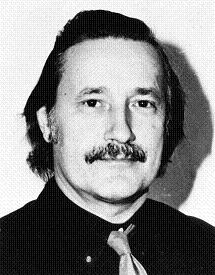
\includegraphics[scale=.7]{Strachey.jpg}
\caption{Christopher Strachey}
\end{subfigure}
\qquad\qquad
\begin{subfigure}{.3\textwidth}\centering\vspace*{-2ex}
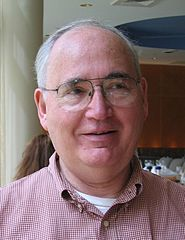
\includegraphics[scale=.85]{DanaScott.jpg}
\caption{Dana Scott}
\end{subfigure}
\caption{지시적 의미구조의 원조인
         크리스토퍼 스트래치와 데이나 스콧 \\
         {\footnotesize(사진 출처:
              \texttt{chessprogramming.org}, 위키미디어 공용)}
	 \label{fig:StracheyScott} }
\end{figure}

지시적 의미구조는 실용적 응용보다는 가장 원론적인 의미구조를 정의함으로써
의미구조 자체의 존재가능성을 비롯한 대상 언어의 이론적 성질을 탐구하기 위한
목적으로 정의하는 경우가 많다. 앞서 살펴본 정규식의 지시적 의미구조도
문자열의 집합이라는 가장 원론적인 형식언어이론에 바탕을 둔 정의이다.
이러한 의미구조의 장점은 이미 그 성질이 명확히 규명되어 있는 수학적 대상을
활용하므로 이론적 성질의 탐구에 적합하다는 것이다. 예를 들면
정규식에서 \VERT 연산자의 의미가 $ \llbracket r_1\VERT r_2\rrbracket
= \llbracket r_1\rrbracket\cup\llbracket r_2\rrbracket$로 정의되고,
집합론에서 합집합은 교환법칙과 결합법칙이 성립함이 잘 알려져 있으므로
정규식의 \VERT 연산도 자연히 교환법칙과 결합법칙이 성립할 수 밖에 없다.
하지만 이런 의미구조는 컴퓨터에 그대로 옮겨 실행하는 등의 실용적 용도에는
잘 맞지 않는다. 그림\;\ref{fig:RegexSynSem}에 나타난 정규식의
클레이니 별표 연산의 의미구조 정의에 따르면 $r^{*}$의 의미가 무한집합에
대응될 수 있으므로 이를 그대로 컴퓨터로 옮기는 것은 적합하지 않다.

\begin{figure}
\begin{align*}
\llbracket\,\cdot\,\rrbracket
 ~:~& \mathcal{R} \to (\Sigma^{*} \to \textbf{Bool})
\\
\llbracket \varnothing \rrbracket(x)   &~=~ \text{False} \\
\llbracket\,\varepsilon\,\rrbracket(x) &~=~ x=\varepsilon \\
\llbracket\,a\,\rrbracket(x)           &~=~ x=a \\
\llbracket r_1 \VERT r_2 \rrbracket(x) &~=~
 \llbracket r_1\rrbracket(x) \lor \llbracket r_2\rrbracket(x)\\
\llbracket\,r_1 \, r_2\,\rrbracket(x) &~=~
  \exists\,x_1\,x_2 \;\text{such that}\; x=x_1x_2,~
  \llbracket r_1\rrbracket(x_1) \land \llbracket r_2\rrbracket(x_2)
  = \text{True} \\
\llbracket\, r^{*} \,\rrbracket(x) &~=~
 \llbracket\,\varepsilon\,\VERT\,r\,r^{*}\,\rrbracket(x)
\end{align*}
\caption{정규식을 문자열 판별함수에 대응시키는
         지시적 의미구조\label{fig:RegexDenoSem}}
\end{figure}

한편, 필요에 따라 실용적 활용에 더 적합한 지시적 의미구조를
정의할 수도 있다. 그림\;\ref{fig:RegexDenoSem}은 정규식에 대한
또 다른 지시적 의미구조로 이번에는 정규식의 의미를 문자열의 집합이
아닌 문자열을 판별하는 함수에 대응시킴으로써 정의하고 있다. 기본적인
세 종류의 정규식의 경우, 널($\varnothing$)은 무조건 거짓인 상수함수,
엡실론($\varepsilon$)은 입력 문자열이 $\varepsilon$일 때만 참인 함수,
알파벳 심볼($a$)은 입력 문자열이 지정된 심볼일 때만 참인 함수로 그
의미가 정의된다. 정규식 연산을 사용한 복합적 정규식의 의미는
그 부분을 구셩하는 정규식의 의미에 대응되는 함수를 이용해 정의된다.
$r_1\VERT r_2$의 의미는 입력 문자열이 $r_1$이나 $r_2$ 의미에 대응되는
판별함수 둘 중 어느 것 하나라도 만족하면 참인 함수로 정의된다.
$r_1\,r_2$의 의미는 입력을 적절히 두 부분으로 잘라 앞부분을 $r_1$의
판별함수에 뒷부분을 $r_2$의 판별함수에 적용했을 때 그 둘 다
만족할 경우에 참인 함수로 정의된다. 클레이니 별표로
이루어진 정규식은 앞서 \ref{sec:regex}절에서 설명한 공식
$r^{*} \equiv \varepsilon\VERT rr^{*}$를 이용해 정의된다.

그림\;\ref{fig:RegexDenoSem}의 의미구조는 컴퓨터 프로그램으로 그리
어렵지 않게 옮길 수 있다. 다른 부분은 의미구조 정의를 거의 그대로
옮기면 되고, 이이붙이기 연산으로 이루어진 $r_1\,r_2$의 의미구조에서
입력 $x$를 ``적절히'' $x_1$과 $x_2$로 자르는 부분만 약간 생각이 필요하다.
효율을 고려하지 않는다면 단순무식하게 모든 경우를 시도해 보면 된다.
예컨대, 세 개의 심볼로 이루어진 입력 문자열 $abc$를 두 부분으로 자르는
모든 경우의 수는 $\varepsilon$과 $abc$, $a$와 $bc$, $ab$와 $c$, $abc$와
$\varepsilon$ 이렇게 넷이다. 그 중 어느 하나라도
$\llbracket r_1\rrbracket(x_1) \land \llbracket r_2\rrbracket(x_2)$를
만족하면 참으로, 즉 문자열 $abc$가 정규식 $r_1\,r_2$를 만족한다고
판별하도록 프로그래밍하면 된다.

필요하다면, 더 효율적인 컴퓨터 프로그램으로 옮길 수 있는 정규식의
지시적 의미구조를 정의하는 것도 얼마든지 가능하다. 아이디어는
지시함수가 문자열을 한꺼번에 처리하는 다소 추상적인 함수에 정규식을
대응시키는 대신에, 기호를 최대 하나씩만 읽어 처리하는 가상적인 기계에
대응시키자는 것이다. 이렇게 하면 $r_1\,r_2$의 의미구조에서 문자열을
두 부분으로 적절히 나누는 지점을 찾고자 비효율적으로 모든 가능성을
다 시도해 보지 않아도 된다. 계산이론 또는 오토마타이론에 익숙한 독자라면
방금 언급한 기계란 다름아닌 유한오토마타(finite automata, FA) 혹은
유한상태기계(finite state machine, FSM)임을 알 것이다. 이 내용은
표준적인 계산이론 혹은 오토마타이론 교재\cite{Sipser2013,Hopcroft2007}에서
상세히 잘 정리하고 있는 내용이므로 여기서 직접 다루지는 않겠다.
다만, 여기서 짚고 넘어가고 싶은 것은, 집합이나 함수 같은 비교적
추상적인 수학적 대상이 아닌, 이정도로 구체적인 가상적 기계 혹은
기계의 설계도에 대응시키는 지시함수(denotation function) 또는
의미값함수(semantic evaluation funciton)는 ``컴파일러''로
볼 수 있다는 점을 환기하고자 한다. 컴파일러는 비교적 추상적인
고급언어를 기계의 동작에 가까운 저급언어로 옮기는 번역기다.
이를 다른 관점으로 보면 기계가 어떻게 동작해야 하는지 구체적인
지침으로 이루어진 특화된 가상의 기계를 생성하는 것으로 볼 수도 있다.
이를테면 공장에서 사칙연산 등에 특화된 탁상용 계산기라는 물리적 기계를
만들어내는 대신, 고급언어로 작성된 탁상용 계산기 소스코드를 컴파일하면
범용 컴퓨터가 실행시켜줄 수 있는 가상의 탁상용 계산기에 해당하는
소프트웨어가 만들어지는 것이다. 마찬가지로 정규식으로부터 해당 정규식을
만족하는 문자열 처리에 특화된 유한오토마타를 생성한다면
이는 명실상부한 정규식의 컴파일러이며, 실제로 이러한 정규식 컴파일러를
내장한 도구가 바로 lex\cite{lex1990}와 같은
어휘분석기 생성기(lexical analyzer generator)다.

\begin{figure}\centering
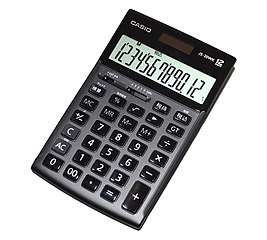
\includegraphics[scale=.4]{DeskCalculator.jpg}\qquad
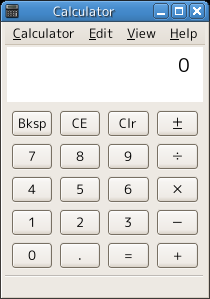
\includegraphics[trim={0 20pt 0 0},clip,scale=.3]{Gcalc.png}\qquad\qquad
\caption{물리적 탁상용 계산기와 소프트웨어 탁상용 계산기\\
         {\scriptsize(이미지 출처: 위키미디어 공용)}}
\end{figure}

이 절에서 지금까지 살펴본 바와 같이 하나의 대상 언어에 지시적 의미구조를
여러 가지로 정의하는 것이 가능하며 또 유용하다. 다만 이런 의미구조들끼리
서로 호환되는지, 기준으로 삼을 만한 가장 원론적인 의미구조와 비교해
어긋나는 부분은 없는지 물샐틈없이 엄밀하게 논리적으로 증명할 필요성이 있다.
활용 목적에 따라 편리한 대로만 정의한다면 모양새 혹은
문법구조만 같을 뿐 의미가 호환되지 않아 실제로는 다른 언어를 표현하면서도
서로 같은 언어를 다룬다고 착각하게 될지도 모르기 때문이다. 이 책의 내용을
엄밀한 이론적 기술을 강조하는 방향으로 구성하지 않았으므로 그런 증명까지
다루지 않겠지만 확실하게 짚고 넘어가야 하는 중요한 사안이라는 점에 대해서는
재차 강조하고 싶다. 이 장에서 다루는 정규식과 관련한 더 자세한 이론적
성질의 증명에 관해서는 계산이론이나 오토마타이론을 다루는
교재\cite{Sipser2013,Hopcroft2007}를, 그 외의 프로그래밍언어 일반에
활용되는 논리적 방법론에 대한 소개는 \citet{PFPL2nd}의 교재를 참고하라.


\section{동작과정 의미구조}
\index{의미구조!동작과정 의미구조}%
\index{semantics!operational semantics}%
\index{동작과정 의미구조|see{operational semantics}}%
\index{denotational semantics|see{동작과정 의미구조}}%
동작과정 의미구조(operational semantics)\cite{Plotkin1981sos}는
프로그램의 의미를 수학적 구조 등 외부의 대상에 지시함으로써 찾는 것이
아니라 프로그램이 계산되는 과정 자체를 프로그램의 의미로 삼는 방식의
의미구조를 말한다. 철학적으로는 의미가 대상에 내재된 것이 아니라 대상들의
관계 속에서 찾아야 한다는 구조주의적 관점과 일맥상통하는 측면이 있다.
참고로 구조주의는 (자연)언어를 기호(sign)의 체계(system), 즉 기호들의
상호관계에 기반한 구조로 이해해야 한다는 소쉬르\cite{Saussure1916}의
언어철학적 관점에서 그 기원을 찾을 수 있다. 이 절에서는 구체적인
사례로서 정규식에 대한 동작과정 의미구조를 어떻게 정의하는지 알아볼
것이다. 그에 앞서, 의미구조 정의에 활용할 몇 가지 기본 개념과
언어의 문자열에 대한 미분에 대해 먼저 소개한다.

\begin{figure}\centering
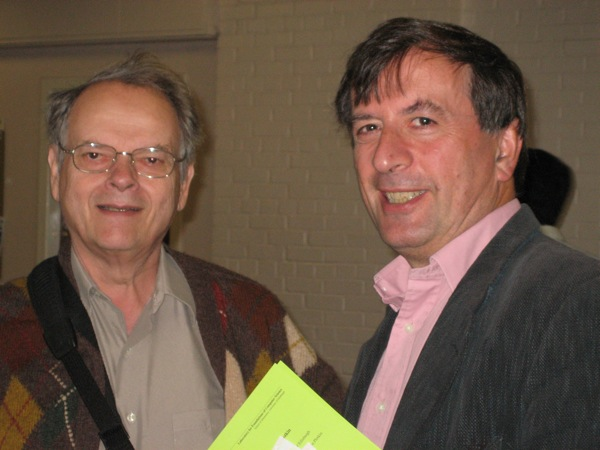
\includegraphics[trim={0 100pt 0 0},clip,scale=0.66]{ReynoldsPlotkin.jpg}\\
{\footnotesize(사진 출처:
\url{https://www.lfcs.inf.ed.ac.uk/events/plotkin-symposium/})}
\caption{동작과정 의미구조의 원조인 고르돈 플롯킨(Gordon D. Plotkin, 우)과
다형 람다계산법(polymorphic $\lambda$-calculus, a.k.a. System F)을
고안한 존 레이놀즈(John C. Reynolds, 좌)의 2006년 사진}
\end{figure}

\subsection{언어와 정규식의 미분}
문자열을 $z=xy$로 아무렇게나 두 부분으로 나눌 때 나올 수 있는
$x$를 앞부분(prefix) $y$를 뒷부분(suffix 또는 postfix)이라 하는데,
문자열 전체나 빈 문자열이 될 수도 있다. 예컨대, $ab$의 가능한 모든
앞부분은 $\varepsilon,a,ab$이며 뒷부분은 $ab,b,\varepsilon$이다.
이어붙이기와 반대로 문자열의 앞부분이나 뒷부분을
떼어내는 연산을 $x^{-1}$로 표기하며 $x^{-1}\,xy = y = yx\,x^{-1}$와
같이 사용한다. 단, 앞부분이나 뒷부분이 $x$와 일치하지 않는 문자열에
대해서는 $x^{-1}$를 적용할 수 없다. 앞부분을 떼내는 연산의 대상을
하나의 문자열이 아닌 문자열 집합, 즉 언어로 확장한 개념이 바로 언어에
대한 미분(그림\;\ref{fig:Brzozowski})이다.
즉, 언어 $L$의 문자열 $x$에 대한 미분이란 $L$에서 앞부분이 $x$인
문자열만 골라 앞부분 $x$을 떼어내고 남은 뒷부분으로 이루어진 언어이다.
예컨대, $(ab)^{-1} \{aa,aab,aabc,ab,abc,abcd\} = \{\varepsilon, c, cd\}$.
언어의 미분을 브쇼조브스키가 최초로 생각한 것은 아니지만,
$x^{-1} \llbracket\,r\,\rrbracket = \llbracket\,r' \rrbracket$를
만족하는 정규식의 미분\footnote{정규식 미분은 $D_a r$나
    $\partial_a r$가 일반적 표기지만
    여기서는 수학에서의 편미분 표기를 차용했다.}
$\partial_{}r/\partial x = r'$을
정의하는 등의 연구 업적을 남겼다. 그래서 정규식에 대한 미분을
브쇼조브스키 미분(Brzozowski derivative)이라 부르기도 한다.
참고로 언어에 대한 미분은 다음의 성질이 성립하며
\begin{enumerate}\tightlist
 \item $\varepsilon \in\,x^{-1} L$\,이면 $x\in L$
      ($\,\because\, x^{-1}x \,=\, \varepsilon\,$)
 \item $\varepsilon^{-1} L \;=\; L$
 \item $(x_1x_2)^{-1} L \;=\; x_2^{-1}(x_1^{-1} L)$
\end{enumerate}
따라서 정규식의 미분도 그에 대응되는 다음의 성질이 성립한다.
\begin{enumerate}\tightlist
 \item $\varepsilon \in \llbracket\,\partial_{}r/\partial x\,\rrbracket$이면
       $x\in \llbracket\,r\,\rrbracket$
 \item $\partial_{}r/\partial\varepsilon \;\equiv\; r$
 \item $\partial_{}r/\partial(x_1\,x_2) \;\equiv\;
        \partial(\partial_{}r/\partial x_1)/\,\partial x_2$
\end{enumerate}
이 절에서는 정규식의 미분을 동작과정 의미구조로 정의하는 데
집중할 것이다. 그 외에 브쇼조브스키가 정규식 미분에 대한
연구한 내용에 대해 조금 더 알아보려면 그의 연구성과\cite{Brzozowski64}를
알기쉽게 요약하여 정리한 논문\cite{Owens09REderivRE}을 참고하라.

\begin{figure}\centering
언어 $L\subset2^{\Sigma^{*}}$의 문자열 $x\in\Sigma^{*}$에 대한 미분:~
$x^{-1} L ~=~ \{\,y \mid xy\in L\,\} \qquad ~~ $\\[1.1ex]
\begin{subfigure}{.2\textwidth}
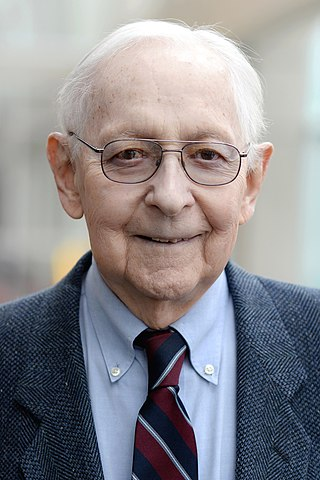
\includegraphics[trim={0 50pt 0 0},clip,scale=1.25]{JanuszBrzozowski.jpg}
\end{subfigure}\qquad\quad
\begin{subfigure}{.65\textwidth}
\!\!정규식의 미분 공식:\\[.7ex]
\( \partial\varnothing\!/\partial a = \varnothing \qquad\quad~\;
   \partial a/\partial a = \varepsilon \) \\[.6ex]
\( \partial\varepsilon/\partial a = \varnothing \qquad\qquad
   \partial b/\partial a = \varnothing \) (단, $a\neq b$)\\[.6ex]
\( \partial(r_1\VERT r_2)\!/\partial a = \partial r_1/\partial a \VERT
                                       \partial r_2/\partial a \)\\[.6ex]
\( \partial(r_1\,r_2)\!/\partial a = (\partial r_1/\partial a)r_2 \VERT
                                 \nu(r_1)(\partial r_2/\partial a) \)\\[.6ex]
\( \partial\,r^{*}\!/\partial a = \partial(rr^{*})\!/\partial a \)\\[.8ex]
\( \partial r/\partial \varepsilon = r \qquad\quad
   \partial r/\partial (ax) = \partial (\partial r/\partial a)/\partial x\)
\end{subfigure}\\[1ex]
\( \nu,\varsigma:\mathcal{R}\to\mathcal{R} \qquad\quad
   \nu(\varnothing) = \varnothing \qquad\quad
   \nu(\varepsilon) = \varepsilon \qquad\quad
   \nu(a) = \varnothing \)\qquad$\phantom{A}$\\[.6ex]
\( \nu(r_1\VERT r_2) = \varsigma(\nu(r_1)\VERT\nu(r_2)) \qquad
   \nu(r_1r_2) = \varsigma(\nu(r_1)\nu(r_2)) \qquad
   \nu(r^{*}) = \varepsilon \)\\[1.2ex]
\( \varsigma(\varnothing\VERT r) = r = \varsigma(r \VERT\varnothing) \quad
   \varsigma(\varepsilon\VERT\varepsilon) = \varepsilon \quad
   \varsigma(\varnothing r) = \varnothing = \varsigma(r \varnothing) \quad
   \varsigma(\varepsilon\,r) = r = \varsigma(r\,\varepsilon) \)\\[.7ex]
(위에 해당되지 않는 다른 모든 경우의 정규식 $r$에 대해서는 $\varsigma(r) = r$\,)
\caption{야누스 브쇼조브스키(Janusz Brzozowski)가 연구한 \\
         언어 및 정규식의 문자열에 대한 미분
         {\scriptsize(사진 출처: 위키미디어 공용)}
         \label{fig:Brzozowski}}
\vspace*{-1ex}
\end{figure}

브쇼조브스키가 정리한 정규식의 미분이 그림\;\ref{fig:Brzozowski}에
나타나 있다.\footnote{브쇼조브스키의 연구 및 관련 후속 연구에는
이 책에서 다룬 정규식의 세 가지 연산 외에도 교집합이나 여집합 연산 등을
포함한 소위 확장된 정규식(extended regular expression)을 다루지만 여기서는
정규언어를 표현하기에 충분한 최소한의 세 가지 연산에 대해서만 다룬다.}
정규식의 각 요소(널, 엡실론, 알파벳 심볼, 합집합, 이어붙이기,
클레이니 별표)를 하나의 기호($a$)에 대해 미분하는 공식이 차례로 나열되어
있으며, 마지막 두 공식은 각각 길이 0인 빈 문자열($\varepsilon$)과 길이
1이상의 문자열($ax$)에 대한 미분 공식이다.

각 요소의 기호 하나에 대한 미분 공식의 원리를 설명하자면 다음과 같다.
\begin{itemize}\tightlist
 \item 널($\varnothing$)과 엡실론($\varepsilon$)은 그 의미상
       맨 앞에서 하나의 기호를 떼낼 수 있는 (즉, 길이 1이상의)
       문자열을 포함할 수 없으므로 미분 결과가 널이다.
 \item 알파벳 심볼의 미분 공식은 둘로 나뉘어 작성되어 있는데,
   정규식 심볼과 똑같은 기호로 미분하는 경우($\partial a/\partial a$)는
   엡실론($\varepsilon$)이며
   다른 기호로 미분하는 경우($\partial b/\partial a$)는
   널($\varnothing$)이다.
 \item 합집합한 정규식의 미분은 각각을 미분한 결과를 합집합한 정규식이다.
 \item 이어붙인 정규식 $r_1\,r_2$의 미분은
       $\varepsilon\notin\llbracket r_1\rrbracket$이면 그냥
       $r_1$의 미분 결과에 $r_2$를 이어붙이면 된다.
       그런데 $\varepsilon\in\llbracket r_1\rrbracket$인 경우는
       정규식에 대응되는 문자열의 첫 글자가 $r_1$이 아닌 $r_2$에
       해당할 수도 있으므로 $r_2$의 미분 결과도 합집합한다.
 \item 클레이니 별표로 이루어진 정규식 $r^{*}$의 미분은
       $r^{*}\equiv \varepsilon\VERT rr^{*}$를 이용한다.
       그런데 엡실론($\varepsilon$)의 미분은 널($\varnothing$)이므로
       $rr^{*}$만 미분하면 된다.\vspace*{-1ex}
\end{itemize}
참고로 정규식의 미분공식(그림\;\ref{fig:Brzozowski}) 및
큰걸음과 작은걸음 의미구조(그림\;\ref{fig:ReDerivBigSmallSem})에서
이어붙이기 연산으로 이루어진 정규식($r_1\,r_2$)을 다룰 때 나타나는
도우미 함수 $\nu:\mathcal{R}\to\mathcal{R}$의 성질은
$\varepsilon \in \llbracket r \rrbracket$인 경우에만
$\nu(r)=\varepsilon$이며 그렇지 않은 경우에는
$\nu(r)=\varnothing$이다. 따라서 $r_1\,r_2$의 미분 공식의 좌변
$(\partial r_1/\partial a)r_2\VERT\nu(r_1)(\partial r_2/\partial a)$는
$\varepsilon \in \llbracket r_1 \rrbracket$인 경우에는
$\nu(r_1)=\varepsilon$이므로
$(\partial r_1/\partial a)r_2\VERT(\partial r_2/\partial a)$와 같고,
$\varepsilon \notin \llbracket r_1 \rrbracket$인 경우에는
$\nu(r_2)=\varnothing$이으로 그냥 $(\partial r_1/\partial a)r_2$와 같다.

문자열에 대한 미분은 기호 하나에 대한 미분을 이용해 계산한다.
빈 문자열에 대해 미분은 앞에서 아무것도 떼어내지 않으므로
원래 정규식 그대로다. 길이 1이상의 문자열에 대한 미분은 앞서 언급한
정규식 미분의 성질 세 가지 중에서 마지막 세 번째 성질을 활용한다.
문자열 $ax$에 대한 미분은 맨 앞의 기호 $a$에 대한 미분 결과를
나머지 문자열 $x$에 대해 미분하여 계산한다.

\subsection{정규식 미분으로 알아보는 동작과정 의미구조의 특징}
지금까지 살펴본 그림\;\ref{fig:Brzozowski}의 공식은
종이에 연필로 수식을 전개할 때 참고하기 좋은 초/중/고등학교
수학 과목에서부터 우리에게 익숙한 형식이다. 그런데 이런 수학 공식 표기는
역사적으로 최초의 컴퓨터 프로그램\cite{Lovelace1843notes}보다 훨씬
오래되었다. 그래서 컴퓨터로 정규식 미분을 자동으로 수행시키려
프로그램으로 옮겨 작성하는 데 가장 적합한 표현 방식은 아닐 것이다.
그림\;\ref{fig:ReDerivBigSmallSem}에는 프로그램으로 옮겨 작성하기에
더 적합한 정규식 미분의 동작과정 의미구조 두 가지를 정의해 놓았다.
첫째는 정규식의 미분을 공식을 가능한 한 계속해 적용한 최종 결과와
관련짓는
\index{의미구조!동작과정 의미구조!큰걸음 의미구조}%
\index{semantics!operational semantics!big-step semantics}%
\index{큰걸음 의미구조|see{big-step semantics}}%
\index{big-step semantics|see{큰걸음 의미구조}}%
큰걸음(big-step) 의미구조이며, 둘째는 정규식의 미분을 기호
하나씩만 미분한 바로 다음 계산 과정과 관련짓는
\index{의미구조!동작과정 의미구조!작은걸음  의미구조}%
\index{semantics!operational semantics!small-step semantics}%
\index{작은걸음 의미구조|see{small-step semantics}}%
\index{small-step semantics|see{작은걸음 의미구조}}%
작은걸음(small-step)
의미구조이다.

\begin{figure}\centering
\begin{subfigure}{\textwidth}
\[
\langle\varnothing, a\rangle \Longmapsto \varnothing
\qquad\qquad
\langle\varepsilon, a\rangle \Longmapsto \varnothing
\qquad\qquad
\langle a, a\rangle \Longmapsto \varepsilon
\quad\quad
\langle b, a\rangle \Longmapsto \varnothing
\]
\[
\inference{ \langle r_1, a\rangle \Longmapsto r_1'
          & \langle r_2, a\rangle \Longmapsto r_2' }{
            \langle r_1 \VERT r_2, a\rangle
            ~\Longmapsto~ \varsigma(r_1'\VERT r_2')}
\qquad
\inference{ \langle r_1, a\rangle \Longmapsto r_1' }{
            \langle r_1\,r_2, a\rangle
            ~\Longmapsto~ \varsigma(r_1'\,r_2)}
            \!^{(\nu(r_1)\,=\,\varnothing)}
\]
\[
\inference{
   \langle r\,r^{*}, a\rangle \Longmapsto r' }{
   \langle r^{*}, a\rangle ~\Longmapsto~ r' }
\qquad\qquad\quad
\inference{ \langle r_1, a\rangle \Longmapsto r_1'
          & \langle r_2, a \rangle \Longmapsto r_2' }{
            \langle r_1\,r_2, a\rangle
            ~\Longmapsto~ \varsigma(\varsigma(r_1'\,r_2)\,\VERT\,r_2')}
            \!^{(\nu(r_1)\,=\,\varepsilon)}
\]
\[
\langle r, \varepsilon\rangle \LONGmapsto r
\qquad\qquad
\inference{ \langle r, a\rangle \Longmapsto r'
          & \langle r', x\rangle \LONGmapsto r'' }{
            \langle r, ax\rangle \LONGmapsto~ r''}
\]
\caption{Big-step semantics:\label{sfig:ReDerivBig}
\fbox{$\cdot\!\Longmapsto\!\cdot
    \,\subset\, (\mathcal{R}\times \Sigma) \times \mathcal{R}$}
\fbox{$\cdot\!\LONGmapsto\!\cdot
    \,\subset\, (\mathcal{R}\times \Sigma^{*}) \times \mathcal{R}$}
\hspace{2ex} }
\end{subfigure}
~\\
\begin{subfigure}{\textwidth}
\[
\langle \varnothing,ax\rangle \longmapsto \langle \varnothing,x\rangle
\qquad\quad
\langle \varepsilon,ax\rangle \longmapsto \langle \varnothing,x\rangle
\qquad\quad
\begin{array}{ll}
\langle a,ax\rangle \longmapsto \langle \varepsilon,x\rangle \\[.75ex]
\langle b,ax\rangle \longmapsto \langle \varnothing,x\rangle
\end{array}
\]
\[
\inference{ \langle r_1, ax\rangle \longmapsto \langle r_1',x \rangle
         \\ \langle r_2, ax\rangle \longmapsto \langle r_2',x \rangle }{
            \langle r_1 \VERT r_2,\,ax \rangle
            \longmapsto \langle\varsigma(r_1' \VERT r_2'), x \rangle }
\quad
\inference{ \langle r_1, ax\rangle \longmapsto \langle r_1',x \rangle }{
            \langle r_1\,r_2,\, ax\rangle
            \longmapsto \langle\varsigma(r_1'\,r_2), x\rangle }
            \!^{(\nu(r_1)\,=\,\varnothing)}
\]
\[
\inference{
   \langle r\,r^{*},\, ax \rangle \longmapsto \langle r',x\rangle }{
   \langle r^{*},\, ax\rangle \longmapsto \langle r',x\rangle }
\qquad~
\inference{ \langle r_1, ax\rangle \longmapsto \langle r_1',x \rangle
         \\ \langle r_2, ax\rangle \longmapsto \langle r_2',x \rangle }{
            \langle r_1\,r_2,\, ax\rangle
            \longmapsto
            \langle\varsigma(\varsigma(r_1'\,r_2)\VERT r_2'),x\rangle }
            \!^{(\nu(r_1)\,=\,\varepsilon)}
\]
\caption{Small-step semantics:\label{sfig:ReDerivSmall}
\fbox{$\cdot\!\longmapsto\!\cdot
    \,\subset\, (\mathcal{R}\times \Sigma^{*})
         \times (\mathcal{R}\times \Sigma^{*})$}
\fbox{$\langle r,\varepsilon\rangle$이면 끝마침} }
\end{subfigure}
~\\
{\small($a$와 $b$가 함께 나타나는 규칙에서는 $a\neq b$임을 가정)}
\caption{정규식 미분의 큰걸음(big-step) 및 작은걸음(small-step) 의미구조
         \label{fig:ReDerivBigSmallSem}}
\end{figure}

동작과정 의미구조는 이항관계(binary relation)로 정의할 수 있다.
그림\;\ref{fig:ReDerivBigSmallSem}에서도
$\Longmapsto$와 $\LONGmapsto$로 큰걸음 의미구조를 정의하고
$\longmapsto$로 작은걸음 의미구조를 정의하고 있다.
큰걸음 의미구조는 일반적으로 계산의 대상이 되는 식을 나타내는 집합
$E$와 결과값의 집합 $V$에 대한 이항관계 $e \Longmapsto v$로 정의되며,
왼항 $e\in E$와 오른항 $v\in V$은 서로 다른 별개의 구조로 이루어진
두 집합($E$, $V$)을 대응시킬 수 있다. 한편, 작은걸음 의미구조를
정의하는 이항관계 $e \longmapsto e'$는 일반적으로 왼쪽과 오른쪽의
두 항 $e,e'\in E$ 모두 같은 계산 대상의 집합($E$)끼리 대응시켜야 한다.
작은걸음 의미구조는 여러 단계로 계산되는 과정의 각 단계를 나타내므로,
계산과정에서 왼항 $e$가 $k$번째 단계의 식이라면
오른항 $e'$는 $k+1$번째 단계의 식이며, 경우에 따라
$e'\longmapsto e''$인 $k+2$번째 단계의 식 $e''$로
한 단계 더 계산과정이 진행될 수도 있다.

동작과정 의미구조의 이항관계는 보통
\index{추론규칙|see{inference rule}}%
\index{inference rule|see{추론규칙}}%
추론규칙(inference rule)의 형태로 정의된다.
추론규칙이란 형식논리(formal logic)를 다루는 증명 체계(proof system)의
증명 과정에 활용하도록 정의한 규칙을 말하며, 이런 형식논리의 증명 체계를
본따 프로그래밍언어의 문법구조(syntax)를 따라 분석하며 의미를 다루는 방식이
동작과정 의미구조라 볼 수 있다. 우리에게 익숙한 논리곱(logical and)에 대한
추론규칙들은 아래와 같이 표현한다. 선 위쪽에는 전제들을, 아래쪽에는
결론을 배치한다. 그리고 선 바로 옆에 규칙의 이름을 표시하기도 한다.
\begin{quote}
\( \inference*[$\land\mathrm{I}$]{A & B}{A \land B}\qquad\qquad
   \inference[$\land\mathrm{E}_1$]{A\land B}{A} \qquad
   \inference[$\land\mathrm{E}_2$]{A\land B}{B} \)
\end{quote}
규칙 $\land\mathrm{I}$는 $A$가 성립하고 $B$가 성립한다는 두 전제로부터
논리곱 $A\land B$가 성립한다는 결론을 증명할 수 있도록 허용한다.
규칙 $\land\mathrm{E}_1$는 논리곱 $A\land B$가 성립한다는 하나의 전제로부터
$A$가 성립한다는 결론을 증명할 수 있도록 허용한다. 마찬가지로,
규칙 $\land\mathrm{E}_2$는 논리곱 $A\land B$가 성립한다는 전제로부터
$B$가 성립함을 증명할 수 있도록 허용한다. 전제가 비어있는 추론규칙을
공리 혹은 공리꼴이라 하는데, 이런 공리나 공리꼴은 가로선을 생략하기도 한다.
예를 들어, 그림\;\ref{fig:ReDerivBigSmallSem}의
$\langle a, a\rangle\!\Longmapsto\!\varepsilon\,$이나
$\langle a, ax\rangle\!\longmapsto\!\langle\varepsilon, x\rangle$는
원래
$\overline{
  \langle a, a\rangle\!\Longmapsto\!\varepsilon}\,$이나
$\overline{
  \langle a, ax\rangle\!\longmapsto\!\langle\varepsilon, x\rangle}$에서
가로선이 생략된 것으로 이해하도 무방하다.

\subsubsection{큰걸음과 작은걸음 의미구조 비교}
큰걸음 의미구조에서는 $e\Longmapsto v$의 성립이 곧 $e$의 ``계산과정''을
제대로 끝마친 것이다. 한편 작은걸음 의미구조에서는 ``계산과정''이 제대로
끝났는지 확인하는 조건을 (누구나 짐작할만한 당연한 내용이 아니라면) 별도로
명시하며, 명시된 종료조건 이외에 계산을 더 진행할 수 없는 경우를 비정상
종료로 간주한다. 예컨대, 정수 산술식의 작은걸음 의미구조를 정의할 때,
정상 종료조건을 정수 리터럴 형태의 식으로 명시하고, 나눗셈 형태의 식
$n_1 / n_2$에 적용할 규칙을 $n_2\neq 0$인 경우에 대해서만 마련했다고 하자.
이 때, $n_1/0$인 형태의 식이 계산과정에 나타난다면 적용가능한 규칙이 없어
계산을 더 진행할 수도 없고 정상 종료조건에 해당하지도 않으므로 비정상적인
계산의 종료로 취급된다. 만일 작은걸음 의미구조에 종료조건이 별도로 제시되지
않았을 때는 더 이상 적용가능한 규칙이 없는 모든 경우를 계산과정의
끝마침으로 취급한다. 참고로, 그림\;\ref{sfig:ReDerivSmall}에 명시한
정규식 미분 계산과정의 종료조건은, 해당 조건이 제시되지 않았더라도 더 이상
적용할 규칙이 없는 경우와 일치하도록 작은걸음 의미구조가 정의되어 있다.
또한, 비정상 종료를 나타내는 형태의 식을 따로 두고 어떤 경우에 비정상 종료할지
명시적으로 나타내는 큰걸음 및 작은걸음 규칙을 포함시켜
프로그램의 비정상 종료를 더 세밀하게 처리하는 의미구조를 정의하기도 한다.

정규식 $(a\VERT b)c^{*}$의 문자열 $acc$에 대한 미분을
그림\;\ref{fig:Brzozowski}의 공식을 활용하여 \vspace*{-2ex}
{\addtolength{\jot}{-1ex}
\begin{align}
     \partial((a\VERT b)c^{*})/\partial(acc)
~=~& \partial(\partial(\partial((a\VERT b)c^{*})
            / \partial a)/\partial c)/\partial c     \label{eqn:ReDeriv1}\\
~=~& \partial(\partial((\varepsilon\VERT\varnothing)c^{*})
            / \partial c)/\partial c                 \label{eqn:ReDeriv2}\\
~=~& \partial(\partial c^{*}/\partial c)/\partial c  \label{eqn:ReDeriv3}\\
~=~& \partial(\partial(cc^{*})/\partial c)/\partial c \label{eqn:ReDeriv4}\\
~=~& \partial(\varepsilon c^{*}\VERT\varnothing(\partial c^{*}/\partial c))
     /\partial c                                     \label{eqn:Rederiv5}\\
~=~& \partial c^{*}/\partial c                       \label{eqn:ReDeriv6}\\
~=~& \partial(cc^{*})/\partial c                     \label{eqn:ReDeriv7}\\
~=~& \varepsilon c^{*}\VERT\varnothing(\partial c^{*}/\partial c)
                                                     \label{eqn:ReDeriv8}\\
~=~& c^{*}                                           \label{eqn:ReDeriv9}
\end{align}
\vspace*{-5ex}\\
}
위와 같이 손으로 풀어 나가듯 계산해 보았다. 이런 계산 과정에서는
계산을 진행하는 사람의 판단에 따라 한 단계의 등식 전개에 같은 공식을
여러 번 반복적으로 적용(식\;\ref{eqn:ReDeriv1})하기도 하며,
공식에 나타나는 형태 그대로 치환하는 데에만 그치지 않고 정규식의 의미상
동치관계($r_1\equiv r_2$)까지 동원해 정규식을 간소화(식\;\ref{eqn:ReDeriv3},
\ref{eqn:ReDeriv6}, \ref{eqn:ReDeriv9})하기도 한다.
반면, 그림\;\ref{fig:ReDerivBigSmallSem}의
동작과정 의미구조에 따른 기계적인 계산 과정에서는 (지시적 의미구조에
바탕을 둔) 정규식의 동치관계 등을 포함해 규칙에 나타나지 않은 계산의
진행은 허용되지 않으며, $\langle r,a\rangle\Longmapsto r'$\,와
$\langle r,x\rangle\LONGmapsto r'$ 형태의 큰걸음
계산과정을 나타내는 유도나무(derivation tree)를 구성하는 각 단계마다
규칙을 정확히 하나씩만 적용해야 한다. 앞서 손으로 계산했던
$(a\VERT b)c^{*}$의 $acc$에 대한 미분을
큰걸음 의미구조(그림\;\ref{sfig:ReDerivBig})에 따라 기계적으로
계산하는 과정을 나타낸 유도나무는 대략 다음과 같은 모양이다.
\vspace*{-2.5ex}
\[%\hspace{-1em}
\setpremisesend{-.25ex}
\inference{
  \inference*{
    \inference{
      \langle a,a\rangle \Longmapsto \varepsilon~ \\
      \langle b,a\rangle \Longmapsto \varnothing
    }{\langle a\VERT b,a\rangle \Longmapsto \varepsilon}
  }{
  \langle(a\VERT b)c^{*}\!,\,a\rangle \Longmapsto c^{*}
  }
& \text{\hspace{-2ex}\small$\!^{(\nu(a\!\VERT\!b)=\varnothing)}$}
& \inference{
    \inference*{\vdots}{
    \langle c^{*}\!,\,c\rangle \Longmapsto c^{*}
    }
  & \inference{
      \inference*{\vdots}{
      \langle c^{*},\,c\rangle \Longmapsto c^{*}
      }
    & \langle c^{*}\!,\,\varepsilon\rangle \LONGmapsto c^{*}
    }{
    \langle c^{*}\!,\,c\rangle \LONGmapsto c^{*}
    }
  }{
  \langle c^{*}\!,\,cc\rangle \LONGmapsto c^{*}
  }
}{
\langle(a\VERT b)c^{*}\!,\,acc\rangle \LONGmapsto c^{*}
}\vspace{-.5ex}
\]
위에서 정규식의 간소화도 사람이 판단해서 임의로 진행하는 것이 아니라,
그림\;\ref{sfig:ReDerivBig}에서 $\Longmapsto$를 정의하는 규칙에
간소화 함수(simplification function) $\varsigma$가 나타나는 곳에서만
$\varsigma$의 정의(그림\;\ref{fig:Brzozowski})에 따라 정규식을
간소화하며 기계적으로 계산을 진행하는 것이다. 예를 들어,
방금 살펴본 유도나무의 왼쪽에 나타나는
$\langle(a\VERT b)c^{*}\!,\,a\rangle \Longmapsto c^{*}$를
유도하는 부분 유도나무에 적용된 규칙의 형태를 그대로 옮기면
$\langle(a\VERT b)c^{*}\!,\,a\rangle
 \Longmapsto \varsigma(\varepsilon c^{*})$이므로
$\varsigma(\varepsilon c^{*}) = c^{*}$로 간소화되는 것이다.

마찬가지 미분을 이번에는 작은걸음 의미구조(그림\;\ref{sfig:ReDerivSmall})에
따라 기계적으로 계산해 보자. 그러려면 아래에 연쇄적인 형태로 작성한
세 단계의 작은걸음 관계($\longmapsto$)가 성립함을 보이는
세 개의 유도나무를 구성해야 한다. \vspace*{-1ex}
\begin{quote}
\( \langle(a\VERT b)c^{*}\!,\,acc\rangle
~\stackrel{\text{\footnotesize\textcircled{\tiny 1}}}{\longmapsto}~
\langle c^{*}\!,\,cc\rangle
~\stackrel{\text{\footnotesize\textcircled{\tiny 2}}}{\longmapsto}~
\langle c^{*}\!,\,c\rangle
~\stackrel{\text{\footnotesize\textcircled{\tiny 3}}}{\longmapsto}~
\langle c^{*}\!,\,\varepsilon\rangle \) \vspace*{-1.25ex}
\end{quote}
위의 각 작은걸음 관계의 성립을 보이는 유도나무는 다음과 같다.
\begin{quote}
 \textcircled{\small 1}
 $\inference*{
    \inference{
       \langle a,acc\rangle \longmapsto \langle\varepsilon,cc\rangle
     & \langle b,acc\rangle \longmapsto \langle\varnothing,cc\rangle
    }{
    \langle a\VERT b,acc\rangle \longmapsto \langle\varepsilon,cc\rangle
    }
  }{
  \langle(a\VERT b)c^{*}\!,\,acc\rangle \longmapsto
  \langle c^{*},\,cc\rangle
 }$\hspace{-8ex}{\small$\!^{(\nu(a\!\VERT\!b)=\varnothing)}$}
 \\[2.5ex]
 \textcircled{\small 2}
 $\inference*{
    \inference{
       \langle c,cc\rangle \longmapsto \langle\varepsilon,c\rangle
    }{
    \langle cc^{*}\!,\,cc\rangle \longmapsto \langle c^{*}\!,\,c\rangle
    }
    \text{\small$\!^{(\nu(c)=\varnothing)}$\hspace{-6ex}}
  }{
  \langle c^{*}\!,\,cc\rangle \longmapsto
  \langle c^{*},\,c\rangle
 }$
 \qquad
 \textcircled{\small 3}
 $\inference*{
    \inference{
       \langle c,c\rangle \longmapsto \langle\varepsilon,\varepsilon\rangle
    }{
    \langle cc^{*}\!,\,c\rangle \longmapsto \langle c^{*}\!,\,\varepsilon\rangle
    }
    \text{\small$\!^{(\nu(c)=\varnothing)}$\hspace{-6ex}}
  }{
  \langle c^{*}\!,\,c\rangle \longmapsto
  \langle c^{*},\,\varepsilon\rangle
 }$
\end{quote}

같은 언어에 대한 큰걸음과 작은걸음 의미구조는 정상적으로 종료되는 계산식에
대해 같은 계산과정을 나타내도록 동작해야 한다. 정규식 미분의 큰걸음과
작은걸음 의미구조(그림\;\ref{fig:ReDerivBigSmallSem})도 다음의 성질을
만족하도록 정의되어 있다.
\vspace*{-1ex}
\begin{itemize}\tightlist
 \item
  $\langle r,x\rangle\LONGmapsto r'$이면
  $\langle r,x\rangle\longmapsto^{*} \langle r',\varepsilon\rangle$이고,
 \item
  $\langle r,x\rangle\longmapsto^{*} \langle r',\varepsilon\rangle$이면
  $\langle r,x\rangle\LONGmapsto r'$이다. \vspace*{-1ex}
\end{itemize}
위에서 $\longmapsto^{*}$는 0회 이상 연쇄적인 작은걸음($\longmapsto$)
계산과정을 뜻한다. 즉, 여러 번의 작은걸음으로 정상종료 형태의 식에 도달한
경우에 큰걸음으로도 그 식에 해당하는 결과값이 계산되어야 하며, 반대로
큰걸음으로 계산한 결과값에 대해 여러 번의 작은걸음으로도 그 결과값에
해당하는 정상종료 형태의 식에 도달할 수 있어야 한다는 말이다.

\subsection{비결정적 (작은걸음) 의미구조와 합류성}
\index{비결정적 의미구조|see{nondeterministic semantics}}%
\index{nondeterministic semantics|see{비결정적 의미구조}}%
비결정적 의미구조(nondeterministic semantics)란 하나의 계산식에
두 가지 이상의 방법으로 규칙이 적용 가능한 경우가 있어 여러 갈래로
계산이 진행될 가능성이 있는 의미구조를 일컫는다. 우리가 아는
대부분의 수학 공식을 그대로 작은걸음 의미구조로 옮긴다면 자연스럽게
비결정적 의미구조가 될 것이다. 왜냐하면 큰 계산식에 공식을 적용할 수 있는
부분이 여러 곳에 있는 경우 어느 한 곳만이 아니라 그 중 어느 곳에든
적용해 계산을 진행해도 되는 경우가 많기 때문이다. 예컨데,
널($\varnothing$)과 엡실론($\varepsilon$)이 포함된 정규식
$(\varepsilon\VERT \varnothing)(\varnothing\VERT \varepsilon)$을
차근차근 간소화(simplify)하려 할 때 다음과 같이 왼쪽 먼저 할 수도 있고
오른쪽 먼저 할 수도 있는 비결정성이 있으며, 그 다음 단계에서도
엡실론이 이어붙이기에 대한 항등원임을 활용할지 아니면
널이 합집합에 대한 항등원임을 이용할지에 따라 또다시
두갈래씩 계산 방향이 나누어진다.
\begin{quote}
\(
(\varepsilon\VERT \varnothing)(\varnothing\VERT \varepsilon) =
\left<\phantom{\begin{array}{l}.\\[4ex].\end{array}}\hspace*{-4ex}\right.
\begin{array}{l}
  \varepsilon(\varnothing\VERT \varepsilon) =
     \Big<\hspace*{-1ex}
     \begin{array}{l}
       \varnothing\VERT \varepsilon \\
       \varepsilon\varepsilon
     \end{array}
  \\[1ex]
  (\varnothing\VERT \varepsilon)\varepsilon =
     \Big<\hspace*{-1ex}
     \begin{array}{l}
      \varepsilon\varepsilon  \\
      \varnothing\VERT \varepsilon
     \end{array}
\end{array}
\)
\end{quote}
그런데 여러 갈래로 계산을 진행할 수 있더라도 계속 진행하다 보면
어디선가 하나로 합쳐서서 최종 결과는 어떻게든 같아지는 성질을 가진
계산들도 상당히 많다. 바로 위에서 진행시키던 간소화도 계속해 보면
아래와 같이 어떤 갈래로 진행하든 결과는 모두 $\varepsilon$으로
합류한다.
\begin{quote}
\(
(\varepsilon\VERT \varnothing)(\varnothing\VERT \varepsilon) =
\left<\phantom{\begin{array}{l}.\\[4ex].\end{array}}\hspace*{-4ex}\right.
\begin{array}{l}
  \varepsilon(\varnothing\VERT \varepsilon) =
     \Big<\hspace*{-1ex}
     \begin{array}{l}
       \varnothing\VERT \varepsilon \\
       \varepsilon\varepsilon
     \end{array}\hspace*{-1ex}
     \Big>
  \\[1ex]
  (\varnothing\VERT \varepsilon)\varepsilon =
     \Big\langle\hspace*{-1ex}
     \begin{array}{l}
      \varepsilon\varepsilon  \\
      \varnothing\VERT \varepsilon
     \end{array}\hspace*{-1ex}
     \Big>
\end{array}
\left.\phantom{\begin{array}{l}.\\[4ex].\end{array}}\hspace*{-4.5ex}\right>
= \varepsilon
\)
\end{quote}
이와 같이 여러 갈래로 계산이 진행되는 비결정적인 의미구조라도
정상 종료되는 결과값에 와서는 하나로 합류하는 성질을
\index{합류성|see{confluence}}%
\index{confluence|see{합류성}}%
합류성(confluence)이라고 한다. 다시 말하자면, 수학에서 상당수의
대수적 계산식은 합류성을 갖도록 정의된 경우가 많다는 것이다.
작은걸음 의미구조가 비결정적이더라도 합류성을 만족한다면,
정상 종료되는 계산식은 그에 대응되는 큰걸음 의미구조에서
하나의 결과값으로 항상 수렴한다. 정리하면, 합류성은 계산 과정이
여러 갈래로 비결정적이더라도 계산 결과가 존재한다면 하나로
결정되도록 보장하는 성질이다.


\begin{comment}
{
\newcommand{\simpRE}[0]{\mathrlap{~~^{\,_\mathfrak{s}}}\longmapsto}
\begin{multline}
a\\
\varnothing \VERT r \simpRE r \\
r \VERT \varnothing \simpRE r \\
\varnothing\,r \simpRE \varnothing \\
r\,\varnothing \simpRE \varnothing \\
\varepsilon\,r \simpRE r \\
r\,\varepsilon \simpRE r \\
\varnothing^{*} \simpRE \varepsilon \\
\varepsilon^{*} \simpRE \varepsilon \\
\inference{r_1\simpRE r_1'}{r_1 \VERT r_2 \simpRE r_1'\VERT r_2 } \\
\inference{r_2\simpRE r_2'}{r_1 \VERT r_2 \simpRE r_1 \VERT r_2'} \\
\inference{r_1\simpRE r_1'}{r_1\,r_2 \simpRE r_1' r_2 } \\
\inference{r_2\simpRE r_2'}{r_1\,r_2 \simpRE r_1\,r_2'} \\
\inference{r\simpRE r'}{r^{*} \simpRE r'^{*}} \\
b
\end{multline}
}
\end{comment}

동작과정 의미구조에 관해서는 소개할 내용이 더 있지만 앞으로도
이 책에서 동작과정 의미구조를 바탕으로 실행가능한 프로그래밍언어의
구현을 프로그램으로 작성해 보면서 새롭게 필요한 개념이 등장하면
그때 소개하기로 한다. 이 절을 마치며 사족을 달자면, 사실
그림\;\ref{sfig:ReDerivSmall}의 정규식 미분의 의미구조는
표면적인 포장은 분명 작은걸음 의미구조의 형태이기는 하나,
큰걸음 의미구조와 관련성이 잘 드러나면서 프로그램으로 옮기기
편하게 정의하다 보니, 다소 큰걸음의 풍미가 첨가되었다고 볼 수 있다.
전형적인 작은걸음 의미구조로 정의하려면 정규식의 미분
$\partial r/\partial x$를 을 나타내는 식 $r \pdvinfix x$를
정규식의 문법구조에 추가하여
\begin{quote}
$r\in \mathcal{R}_{\partial} ~::=~
 \varnothing ~\mid~ \varepsilon ~\mid~ a ~\mid~
 r\VERT r ~\mid~ rr ~\mid~ r^{*} ~\mid~ r \pdvinfix x$
\end{quote}
위와 같이 같이 확장하고,
미분공식(그림\;\ref{fig:Brzozowski})에 따라 이항관계
$\cdot\!\longmapsto\!\cdot \subset R_{\partial}\times R_{\partial}$를
적절히 정의하되 종료조건이 되는 계산식의 형태는
추가된 미분 연산자($\pdvinfix$)를 포함하지 않는
원래의 정규식 $r\in \mathcal{R}$로 하면 된다.

\section{공리적 의미구조}
\index{의미구조!공리적 의미구조}%
\index{semantics!axiomatic semantics}%
\index{공리적 의미구조|see{axiomatic semantics}}%
\index{axiomatic semantics|see{공리적 의미구조}}%
공리적 의미구조(axiomatic semantics)에 대해서는 이 책에서는 많이 다루지
않으므로 간략히 개념만 설명하고 넘어가겠다. 그렇다고 해서 중요하지 않은
프로그래밍언어의 의미구조 표현 방식이라는 뜻은 아니다. 어떤 관점에서는
공리적 의미구조야말로 지금까지 실용적 활용 사례\footnote{단적으로,
  NASA에서도 활용한다.
  \url{https://ti.arc.nasa.gov/tech/rse/publications/vnv/}}가 가장 많은
의미구조의 표현 방식이라 볼 수도 있다. 역사적으로도 공리적 의미구조의
기원이 되는 이론인 호어 논리(Hoare logic)\cite{Hoare69}의 발표와 함께
프로그램 검증(program verification) 분야가 본격적으로
시작하였다\cite{GSLeeHJKim20Hoare}고 본다. 오늘날에는 호어 논리를
확장한 분리 논리(separation logic)\cite{IshtiaqOHearn01,
OHearnReynoldsYang01}를 프로그램 검증에 활용하는 추세다.

\begin{figure}
\begin{subfigure}{.33\textwidth}
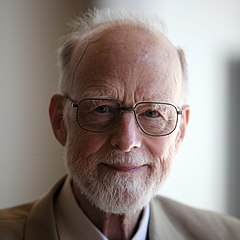
\includegraphics[]{SirTonyHoare.jpg}
\end{subfigure}
\begin{subfigure}{.65\textwidth}\small
호어 논리(Hoare logic) 외에도, 퀵정렬(Quicksort) 알고리듬과
동시에 실행되는 프로세스 사이의 통신을 표현하는 형식언어인
CSP를 고안하였으며, 데이커스트라(Dijkstra)와 함께
구조적 프로그래밍(structured programming)을 주창하며
ALGOL 언어의 설계에도 공헌하는 등 초기 컴퓨터과학의 발전에
크게 기여하였다. ALGOL에 널참조(null reference)라는 개념을
도입하는 바람에 이후 여러 다른 언어에도 쓰이게 되며 수많은
SW버그의 요인이 되는 것을 보고 후회했다는 언급을 하기도 했다.
\end{subfigure}
\caption{Sir Charles Antony Richard Hoare (2011 사진) \label{fig:Hoare}}
\end{figure}


프로그램 검증은 일반적인 검사(testing) 방식의 한계를 극복할 수 있게 한다.
비유하자면 개미는 모두 검다는 성질을 확인하기 위해 10000마리의 개미를
확인해 보니 모두 검은 개미였다 할지라도 10001번째 잡은 개미가 붉은
개미일 수 있듯이, 프로그램이 어떤 성질을 만족한다는 10000개의 테스트를
통과했더라도 또 다른 10001번째 입력으로 실행했을 때 만족하리라는 보장이
없다는 것이 일반적인 검사 방식의 근본적인 한계이다. 프로그램을 실제로
실행하여 구체적인 입력 사례와 그 결과값을 개별적으로 확인하는 일반적인
검사 방식과 달리, 프로그램을 직접 실행하지 않고 그 설계도인 소스코드로부터
수학에서의 증명처럼 모든 가능한 경우에 대해 프로그램이 원하는 성질을
만족함을 보이는 것을 `프로그램 검증'이라 한다. 여기서 ``원하는 성질''이
어떤 내용인지 분명하고 자세하면서도 정확하게 표현하기 위해 고안된
형식논리(formal logic) 체계가 바로 호어 논리이다. 참고로, 프로그램이
의도한 바대로 동작하기 원하는 성질을 분명하고 자세히 표현했다는 뜻에서
그러한 내용을 `명세'(specification)라 일컫는다. 정리하면, 프로그램이
항상 그 명세(specification)대로 동작할 것임을 소스코드로부터 입증하는
것을 `프로그램 검증'이라 하며 이러한 검증에 활용되는 대표적인 형식논리
체계가 `호어 논리'이다.

호어 논리의 문장(statement)은 $\{P\}\,C\,\{Q\}$ 형태로 작성되는데,
$P$, $C$, $Q$의 세 요소로 구성되므로 호어 트리플(Hoare triple)이라고도
부른다. $C$는 명세의 대상이 되는 프로그래밍언어의 문장(statement) 혹은
명령(command)이며, 명세의 내용에 해당하는 ${P}$와 ${Q}$를 각각
전제조건(precondition)과 사후조건(postcondition)이라 한다.
참고로, $C$의 실행에 앞서 만족되어 있어야 할 조건인 $P$와
실행 이후에 만족되어야 할 조건인 $Q$를 그런 의미에서
선행조건(precondition)과 후행조건(postcondition)으로 옮기기도 한다.
실제 프로그램 소스코드보다 일상생활에서 친숙한 내용을 다음과 같은
호어 트리플로 작성해 볼 수 있다.
\begin{quote}\small
\{밥 $n+1$공기 이상 있음\}\;``밥\;1공기\;먹어''\;\{밥 $n$공기 이상 있음\}
~~(단, $n\ge 0$)
\end{quote}
이렇게 선행조건과 후행조건으로 기본적인 명령의 의미구조를 나타내는데,
위의 호어 트리플은 증명해야 할 대상이 아닌 형식논리 체계에서
받아들여야 하는 공리(axiom)로서의 역할을 하기 때문에 이러한 방식으로
프로그래밍언어의 의미구조를 정의하는 것을 `공리적 의미구조'라
일컫는다. 위에서 $n$은 하나의 값으로 정해진 것이 아니라 해당 명령을
사용하는 사례마다 적절히 다른 값으로 구체화할 수 있다. 그러니까 하나로
정해진 공리(axiom)가 아닌 여러 공리를 대표하는 일반적인 공리의 형태를
나타낸다는 뜻에서 공리꼴(axiom schema) 혹은 공리 도식이라고 일컫는다.

(명령형) 프로그래밍언어에서는 여러 문장을 연달아 작성하여 차례대로
실행할 수 있다. 달리 말하자면 명령 $C_1$과 $C_2$를 순차적으로 실행하라는
복합적 명령 $C_1;C_2$를 작성할 수 있다는 이야기다. 따라서 밥 한 공기
먹고 나서 밥을 또 한 공기 먹는 복합적 명령은 다음과 같이 작성하면 된다.
\begin{quote}\small
``밥 1공기 먹어'';``디저트 1그릇 먹어''
\end{quote}
호어 논리에는 이런 복합적 명령에 대한 명세를 다루는 데 유용한
다음의 추론 규칙이 제공된다.
\begin{quote}
\( \inference[composition]{ \{P\}C_1\{R\} & \{R\}C_2\{Q\} }{
                            \{P\}\,C_1;C_2\,\{Q\} } \)
\end{quote}
먼저 실행되는 $C_1$의 후행조건과 다음에 실행되는 $C_2$의 선행조건이
$R$로 일치할 경우 두 명령을 조합(composition)한 $C_1;C_2$에 대한
호어 트리플을 구성할 수 있음을 말한다.

방금 위에서 소개한 규칙에 따라 밥 한 공기 먹고 또 한 공기 더
먹는 복합명령에 대한 호어 트리플을 구성해 보자. 우선 우리가
앞서 살펴본 호어 트리플을, 내용이 길어지므로 이제부터
좀 더 간략한 표기로, 나란히 써놓고 살펴보자.
\begin{quote}\small
$\{\text{밥}\ge n'+1\}\,\text{``밥\,1\,먹어''}\,\{\underline{\text{밥}\ge n'}\}$
\qquad
$\{\underline{\text{밥}\ge n+1}\}\,\text{``밥\,1\,먹어''}\,\{\text{밥}\ge n\}$
\end{quote}
왼쪽과 오른쪽 호어 트리플에서 $n$값이 서로 다를 수 있으므로 한쪽을 $n'$로
구분하였다. 조합(composition) 규칙을 적용하려면 밑줄 친 왼쪽 명령의
후행조건과 오른쪽 명령의 선행조건이 일치해야 하므로, 왼쪽의 $n'$를
$n+1$로 구체화하여 일치시킨 후 아래와 같이 추론 가능하다.
{\small
\[
\inference[]{
  \{\text{밥}\ge (n+1)+1\}\,\text{``밥\,1\,먹어''}\,\{\text{밥}\ge n+1\}
  &
  \{\text{밥}\ge n+1\}\,\text{``밥\,1\,먹어''}\,\{\text{밥}\ge n\}
}{
  \{\text{밥}\ge (n+1)+1\}
  \,\text{``밥\,1\,먹어''};\text{``밥\,1\,먹어''}\,
  \{\text{밥}\ge n\}
}
\]
}
이렇게 복합명령에 대한 호어 트리플 {\small
$\{\text{밥}\ge n+2\}
 \,\text{``밥\,1\,먹어''};\text{``밥\,1\,먹어''}\,
 \{\text{밥}\ge n\}$}을 공리꼴로부터 추론 규칙을 활용해
유도할 수 있음을 살펴보았다. 참고로, 호어 논리에는 연달아 실행하는
순차적 복합문 외에도 (명령형) 프로그래밍언어에 공통적으로 나타나는
조건문과 반복문에 대한 추론규칙들도 추가로 제공된다. 그런 추론 규칙들을
활용하면 공리꼴부터 다양한 프로그램에 대한 공리적 의미구조에 해당하는
호어 트리플을 도출할 수 있다.

지금까지 공리적 의미구조의 기본적인 개념을 다소 피상적인 비유를 통해
최대한 간단히 표면적으로나마 살펴보았다. 이런 공리적 의미구조가
프로그램 검증에 많이 활용되는 까닭은 프로그램 검증 분야의 초기부터
역사를 함께했다는 이유도 있지만 호어 로직 방식 명세의 유연함이라는
장점 또한 하나의 요인이 된다. 호어 트리플의 선행조건과 후행조건을
명세하는 구체적인 형식논리체계는 검증하고자 하는 성질에 적합한 것으로
선택할 수 있다. 또한 프로그램의 모든 의미를 포괄할 필요 없이 집중하고자
하는 성질에 대해서만 명세하고 나머지를 생략하는 것도 얼마든지 가능하다.
예컨대, 메모리를 얼마나 사용하는지 중점적으로 검증할 때에는 계산되는
대부분의 결과값을 무시하고 얼마나 많은 변수가 선언되고 메모리 할당이
일어났는지만을 중심으로 공리적 의미구조를 정의하는 것이 가능하며,
구현된 알고리즘의 복잡도와 관련된 개념을 검증하고자 할 때는
이를테면 비교 연산이나 산술 연산 등 핵심 연산이 얼마나 많이
수행되는지에만 집중하여 표현된 공리적 의미구조를 정의하는 것도 가능하다.

\section*{요점정리}
\begin{itemize}[itemsep=0pt]
 \item 지시적 의미구조(denotational semantics)는 프로그램 $e$의 의미를
       수학적 구조 $\llbracket e\rrbracket$에 대응시킴으로써 정의한다.
       예를 들면 정규식의 지시적 의미구조를 문자열의 `집합'인 언어에
       대응시킴으로써 정의할 수 있다.
 \item 의미구조 괄호 $\llbracket \cdot \rrbracket$로 표기되는
       함수를 지시함수(denotation function) 또는
       의미값함수(semantic evaluation function)이라 한다.
 \item 지시적 의미구조는 원론적인 의미구조를 정의함으로써 대상 언어의
       성질을 이론적으로 규명하기에 적합하다는 장점이 있다.
 \item 하나의 언어에 대한 지시함수를 다르게 정의하여 여러 가지로
       지시적 의미구조를 정의할 수 있으며, 필요에 따라서는 실용적으로
       활용가능한 컴파일러에 해당하는 지시적 의미구조도 정의할 수 있다.
 \item 하나의 언어를 대상으로 하는 서로 다른 의미구조가 서로 어긋남
       없이 일관된 뜻을 나타낸다 엄밀한 이론적 증명이 필요하다.
 \item 동작과정 의미구조(operational semantics)는 프로그램의 의미구조를
       외부의 대상에서 찾지 않고 프로그램이 결과값으로 바뀌어 가는
       계산과정 자체를 의미구조로 정의한다. 따라서 프로그램으로 옮겨
       대상이 되는 언어를 구현하기에 적합한 의미구조의 표현 방식이라 볼 수 있다.
 \item 동작과정 의미구조는 이항관계로 정의할 수 있는데,
       프로그램($e$)을 최종 결과값($v$)과 연관짓는 ($e\Longmapsto v$)
       큰걸음(bit-step) 의미구조와 계산 과정의 계산식($e$)을 바로
       다음 단계의 계산식($e'$)와 연관짓는 ($e\longmapsto e'$)
       작은걸음 의미구조의 두 가지 정의 방식으로 크게 분류할 수 있다.
 \item 큰걸음 의미구조에서는 $e\Longmapsto v$의 성립 자체가 정상적인
       계산의 종료를 의미한다.
 \item 작은걸음 의미구조에서는 계산이 정상 종료되는 계산식의 형태를
       종료조건으로 명시하면 그 이외의 형태로 더 이상 진행할 수 없는
       계산은 비정상 종료로 취급한다.
 \item 같은 언어에 큰걸음과 작은걸음 의미구조를 서로 같은 계산과정을
       표현하도록 정의했다면, 큰걸음으로 $e\Longmapsto v$일 때
       0회 이상의 여러 작은걸음으로 $e\longmapsto \cdots \longmapsto v$이어야 하고,
       반대로 여러 작은걸음 $e\longmapsto \cdots \longmapsto e'$로
       정상종료되는 계산과정은 큰걸음에서도 $e\Longmapsto e'$이며 이 때
       $e'$는 큰걸음에서 최종 계산값의 형태에 부합한다.
 \item 여러 갈래로 진행될 가능성이 있는 계산을 포함하는 작은걸음 의미구조를
       비결정적(nondeterministic)인 의미구조라 하는데, 이 때 정상 종료하는
       계산에 대해서는 항상 갈라졌던 계산이 다시 하나로 합쳐지면서 유일무이한
       결과값으로 수렴한다면 그러한 의미구조는 합류성(confluence)이 있다.
 \item 문자열을 둘로 자르는 모든 경우에 나타날 수 있는 앞쪽을 앞부분(prefix)
       그리고 뒤쪽을 뒷부분(suffix 또는 postfix)이라고 한다.
 \item 문자열의 왼쪽에 $x^{-1}$라 쓰면 앞부분이 $x$인 문자열에서 그 앞부분 $x$를
       떼내고 남은 뒷부분을 계산하는 연산이며 이를 문자열의 집합인 언어($L$)로
       확장한 개념이 바로 언어의 문자열에 대한 미분($x^{-1} L)$이다.
       브쇼조브스키는 문자열의 미분을 기반으로 정의한 정규식의 미분을 연구하였다.
 \item 공리적 의미구조(axiomatic semantics)는 호어 논리(Hoare logic)에서
       그 기원을 찾을 수 있으며, 역사적으로 호어 로직과 함께 프로그램
       검증 분야가 본격적으로 시작되었기에 프로그램 검증에 실용적으로
       가장 활발하게 응용되어 온 방식의 의미구조라 볼 수 있다.
 \item 프로그램 검증이란 프로그램을 실행해 특정 입력 사례에 대해 기대하는
       결과가 계산되는지 알아보는 일반적인 프로그램 검사와 달리 일반적으로
       모든 경우에 프로그램이 어떤 성질을 만족하는지 수학에서의 증명과 같이
       논리적으로 검증하는 접근 방식이다.
 \item 공리적 의미구조는 프로그램($C$)이 실행되기 전에 만족되어야 하는
       선행조건($P$)과 실행 후에 만족될 후행조건($Q$)으로써 프로그램의
       의미를 정의한다. 이렇게 프로그램과 그 선행조건 및 후행조건의
       세 요소로 이루어진 표현 $\{P\}\,C\,\{Q\}$를
       호어 트리플(Hoare triple)이라 한다.
\end{itemize}

\section*{연습문제}
\begin{enumerate}[itemsep=0pt]
 \item 덧셈과 곱셈을 포함하는 계산식에 대한
       큰걸음 의미구조와 작은걸음 의미구조를 정의해 보라.
 \item 앞의 문제에서 정의한 의미구조가 결정적인지 비결정적인지 따져보라.
\end{enumerate}

\section*{탐구과제}
\begin{enumerate}[itemsep=0pt]
 \item 그림\;\ref{fig:RegexDenoSem}를 곧이곧대로 프로그램으로 옮길 경우
       함수의 계산이 끝나지 않는 경우가 발생할 수 있다.
       어떤 경우에 그런지 분석해 보고, 끝나지 않는 계산을 피하려면
       어떤 부분을 신경써야 할지 생각해 보라.
 \item 비결정적인 작은걸음 의미구조를 결정적인 의미구조로 바꾸려면
       어떻게 해야 하는지 알아보라.
 \item 동작과정 의미구조를 설명하는 본문의 끝부분에 더 작은걸음스러운
       정규식 미분의 작은걸음 의미구조를 정의하려면 어떤 방향으로 접근해야
       할지 제시했다. 실제로 구체적인 규칙을 정의해 가며 작은걸음 이런
       방향으로 정규식 미분의 작은걸음 의미구조를 정의해 보라.
 \item 호어 로직을 확장한 분리 논리(separation logic)의 특징과 응용 사례를 조사해 보라.
\end{enumerate}

\chapter{유효범위(Scope)와 타입(Type)}
컴파일러 관련 기술을 논할 때, 구문분석(syntax analysis)을 마치고
가운데단의 중간 코드 생성(intermediate code generation) 및
최적화(optimization)와 뒷단의 코드 생성(code generation)을 하기 전,
앞단의 작업을 마무리하며 진행되는 일련의 작업을 대략
의미분석(semantic analysis)이라 부른다 \cite{Aho2013compilers2nd}.
프로그램에서 이름(name) 혹은 식별자(identifier)가 유효범위(scope)에
맞게 사용되는지, 또 계산식이 타입(type)에 맞게 활용되는지 등에 대한
검사도 여기에 포함되며, 이런 작업을 진행하며 얻은 정보를 (추상)문법나무에
추가적인 속성(attribute)으로 추가하기도 한다. 하지만 그렇다고 해서
보통의 컴파일러에서 소위 `의미분석'으로 분류되는 모든 작업을 원론적으로
문법구조의 영역이 아닌 의미구조의 영역으로 딱 떨어지게 경계지을 수 있는
것은 아니며, 단지 지금까지 프로그래밍언어 구현을 보통 그런 식으로
구성했다는 말이다. 프로그래밍언어에서 유효범위(scope)와 타입(type)은
문법구조(syntax)일까 의미구조(semantics)일까?

\newpage

\section{이름의 유효범위와 문법구조}
변수 등의 이름이 그 유효범위에 맞게 사용되는지는 문맥자유문법(CFG)의
표현 범위를 넘어선 문맥의존문법(CSG)까지 동원하면 형식문법으로 표현
가능하므로 이론적으로는 얼마든지 순수한 문법구조의 영역으로 볼 수 있다.
물론 일반적인 CSG는 프로그래밍언어 구현에서 현실적인 용도로 사용할 만큼
효율적인 알고리듬으로 처리하기 어렵기 때문에 지금까지의 대부분 프로그래밍
언어 구현에서 대략 CFG로 표현 가능한 만큼의 구문분석을 한 뒤에
유효범위 등은 별도로 처리하는 것이 일반적이었던 것이다. 하지만
문맥자유문법의 비교적 온건한 확장\cite{Okhotin2005existence}으로도
이름 유효범위와 같은 기능을 처리할 수 있음이 밝혀져 있으므로, 새로운
언어 구현을 시도한다면 이를 구문분석 과정의 일부로 처리하는 것도
비현실적 접근은 아니다. 이 절에서는 특정 형식문법으로 효과적으로
표현 가능한가에 대한 내용보다는, 어째서 이름 유효범위를 의미구조보다
문법구조로 보는 것이 자연스러운지 직관적인 예시로 설명한다. 또한,
유효범위를 어떤 데이터 구조의 관점에서 접근하면 개념적으로 이해하기도
좋고 구현과 관련한 활용에도 유용한지 소개하려 한다.

\subsection{이름의 유효범위(scope)와 납치(catpure)}
\index{이름의 유효범위|see{scope}}%
\index{scope|see{이름의 유효범위}}%
그림\;\ref{fig:samefun}에는 C/C++ 언어로 1부터 n까지의 합을 계산하는 함수를
처음에는 단순한 반복문으로 작성(그림\;\ref{sfig:samefun1})하고, 이를 여러모로
수정해 보았다. 반복문 정도의 기초적인 프로그램 요소 정도에만 익숙하더라도
원래 함수인 그림\;\ref{sfig:samefun1}과 \texttt{y}를 \texttt{z}로 바꿔친
그림\;\ref{sfig:samefun2}는 똑같은 함수지만, \texttt{y}를 \texttt{n}으로
바꿔친 그림\;\ref{sfig:samefun3}는 전혀 다른 함수라는 것을 한눈에 알아볼 수
있을 것이다. 고정 크기 정수의 넘침(overflow)같은 컴퓨터 하드웨어를 고려한 
정수 표현의 세부사항은 무시하고 수학적으로 이상적인 정수의 연산만을 생각한다면,
그림\;\ref{sfig:samefun1}과 \ref{sfig:samefun5}는 조금 다른 측면에서
``같은'' 함수이다. 그림\;\ref{sfig:samefun1}과 \ref{sfig:samefun2}는
그냥 생긴 것만 봐도 같은, 즉 문법구조적으로도 거의 같지만,
그림\;\ref{sfig:samefun1}과 \ref{sfig:samefun5}는 정수 덧셈, 곱셈, 나눗셈의
성질 등 수학적 의미를 따져보았을 때 의미구조상 같다고 정리할 수 있다.

\begin{figure}
\lstset{numbers=left,numberstyle=\scriptsize\color{gray}}
\begin{subfigure}[b]{.4\textwidth}
\begin{lstlisting}
int f(int n) {
  int y = 0;
  for (int x = 1; x <= n; x++)
      y += x;
  return y;
}
\end{lstlisting}
\vspace*{-\baselineskip}
\caption{n까지 더하는 함수\label{sfig:samefun1}}
\end{subfigure}
\hfill
\begin{subfigure}[b]{.4\textwidth}
\begin{lstlisting}
int f(int n) {
  int z = 0;
  for (int x = 1; x <= n; x++)
      z += x;
  return z;
}
\end{lstlisting}
\vspace*{-\baselineskip}
\caption{\texttt{y}를 \texttt{z}로 바꿔치기\label{sfig:samefun2}}
\end{subfigure}
\\[1ex]
\begin{subfigure}[b]{.4\textwidth}
\begin{lstlisting}
int f(int n) {
  int n = 0;
  for (int x = 1; x <= n; x++)
      n += x;
  return n;
}
\end{lstlisting}
\vspace*{-\baselineskip}
\caption{\texttt{y}를 \texttt{n}으로 바꿔치기\label{sfig:samefun3}}
\end{subfigure}
\hfill
\begin{subfigure}[b]{.4\textwidth}
\begin{lstlisting}
int f(int n) {
  int y = n - 100;
  for (int x = 1; x <= n; x++)
      y += x;
  return x;
}
\end{lstlisting}
\vspace*{-\baselineskip}
\caption{\texttt{0}을 \texttt{n-100}으로 바꿔치기$\hspace{-7ex}$\label{sfig:samefun4}}
\end{subfigure}
\\[1ex]
\begin{subfigure}[b]{.4\textwidth}
\begin{lstlisting}
int f(int n) { return (n + 1) * n / 2; }
\end{lstlisting}
\vspace*{-.6\baselineskip}
\caption{가우스의 덧셈 공식\label{sfig:samefun5}}
\end{subfigure}
\caption{요렇게 저렇게 바꾸면 무엇이 무엇이 똑같은가?\label{fig:samefun}}
\end{figure}

그렇다면 그림\;\ref{sfig:samefun2}와 비슷한 방식으로 수정한 
그림\;\ref{sfig:samefun3}은 어째서 우리가 한눈에 보고 다른 함수라고 판단했을까?
프로그래밍에 대해 잘 모르는 친구가 이런 식으로 물어보면 뭐라고 설명할까
잠깐 고민하다가, 저렇게 고치면 1부터 n까지 합이 아닌 엉뚱한 계산을 한다고,
아마도 설명하려 들 것이다. 그런데 설명하려고 잠깐 고민하기 전부터
기초적인 프로그래밍이라도 직접 해본 사람이라면, 이미 이건 함수의 내용을
따지기 전에 뭔가 달라졌다고 직감했을 것이다. 이런 직감을 전문용어를
동원해 설명하자면 변수의 이름을
\index{바꿔치기|see{substitution}}%
\index{치환|see{substitution}}%
\index{substitution|see{바꿔치기}}%
\index{substitution|see{치환}}%
바꿔치기(substitution) 혹은 치환하면서
원래 함수에서
\index{이름의 유효범위 묶음|see{name binding}}%
\index{name binding|see{이름의 유효범위 묶음}}%
이름이 유효범위에 묶여있던 (name binding) 구조까지도 의도치
않게 바꿔버린 것이다. 그림\;\ref{sfig:samefun2}에서는 변수 \texttt{y}를 선언하고
사용하는 모든 곳에서 새로운 이름 \texttt{z}로 바꿔치더라도 이름이 유효범위에
묶여있는 구조는 변하지 않았다. 하지만 그림\;\ref{sfig:samefun3}에서 \texttt{y}를
\texttt{n}으로 바꿔치면, 원래 함수(그림\;\ref{sfig:samefun1})에서 3째줄의
\texttt{x\,<=\,n}에 사용되는 \texttt{n}은 1째줄에 함수의 매개변수(parameter)로
선언된 \texttt{n}에 묶여있었는데 이름을 바꿔친 다음(그림\;\ref{sfig:samefun3})에는
같은 3째줄의 \texttt{x\,<=\,n}에서 \texttt{n}이 이제는 함수의 지역 변수로 선언된
2째줄의 \texttt{int n}에 묶여있다. 즉, 3째줄의 \texttt{n}이 원래 함수 전체
유효범위에 묶여있던 이름이였는데 수정한 다음에 함수의 일부인 2째줄 이후의
더 좁은 유효범위에 묶여있는 이름이 되어버린 것이다. 이렇게 의도치 않게
더 좁은 유효범위에 갇히는 상황을 이름이 납치(capture)되었다고도 한다.

그림\;\ref{sfig:samefun4}에서는 그림 자체에 나타나 있지 않은 상황을 추가로
가정하자면, 함수 바깥에 프로그램의 다른 부분에서 상수로 사용하는 전역변수
\texttt{n}의 값이 \texttt{100}으로 정의되어 있다고 하자. 그러면 함수 바깥의
다른 곳에서는 \texttt{n-100}의 값이 \texttt{0}이므로 같은 값의 식끼리 치환을
시도한 상황이 된다. 그런데 하필 함수 파라메터의 이름이 \texttt{n}으로 전역변수의
이름과 겹쳐서 이 함수 안으로 들어온 2째줄의 \texttt{n-100}에서 \texttt{n}은
더이상 원래 의도했던 전역 유효범위가 아닌 더 좁은 범위의 함수 유효볌위에 묶인
이름이 되어버린다. 유효범위가 의도한 것보다 더 좁은 곳에 묶인다는 점은 같지만
앞서 그림\;\ref{sfig:samefun3}에서는 내부적으로 사용하는 이름을 (더 가독성이
좋은 이름으로 새로 짓거나 하는 등의 이유에서) 일괄적으로 바꾸려다 의도치 않은
이름의 납치가 발생한 상황이라면 이번 경우는 바깥에서 사용하던 프로그램식을
안으로 옮겨 사용하려다 이름의 납치가 발생한 상황이다.

이렇듯 단순히 문서편집기에서 문자열을 다른 문자열로 바꿔치기(substitution)하는
방식으로는 이름 납치가 발생할 위험성이 있다. 그래서 기존에 작성했던 소스코드의
구조개선을 돕는 리팩토링(refactoring) 도구 등의 프로그래밍언어 소스코드의
문법구조를 따라 안전하게 일괄적으로 치환하는 기능이 필요한 도구에는
\index{납치없는 바꿔치기|see{capture avoiding substitution}}%
\index{capture avoiding substitution|see{납치없는 바꿔치기}}%
``납치없는 바꿔치기''(capture avoiding substitution)를 구현해야
한다. 예를 들면 방금 살펴본 그림\;\ref{sfig:samefun4}에서는 \texttt{n-100}을
함수 안으로 옮겨오기 전에 이름 납치의 가능성을 인지하고 함수 파라메터 이름을
\texttt{n}에서 \texttt{m}과 같은 겹치지 않는 이름으로 먼저 일괄적으로 바꿔
놓으면 된다. 물론 이렇게 내부적으로 이름을 치환하는 중에도 이름 납치가 발생하지
않도록 하면서 말이다.

\subsection{이름의 유효범위 묶음(name binding)을 포함한 문법구조의 같음}
\index{이름의 유효범위 묶음}%
\index{name binding}%
\begin{figure}\centering
\begin{subfigure}{.25\textwidth}
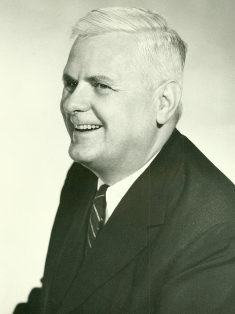
\includegraphics[scale=1]{AlonzoChurch.jpg}
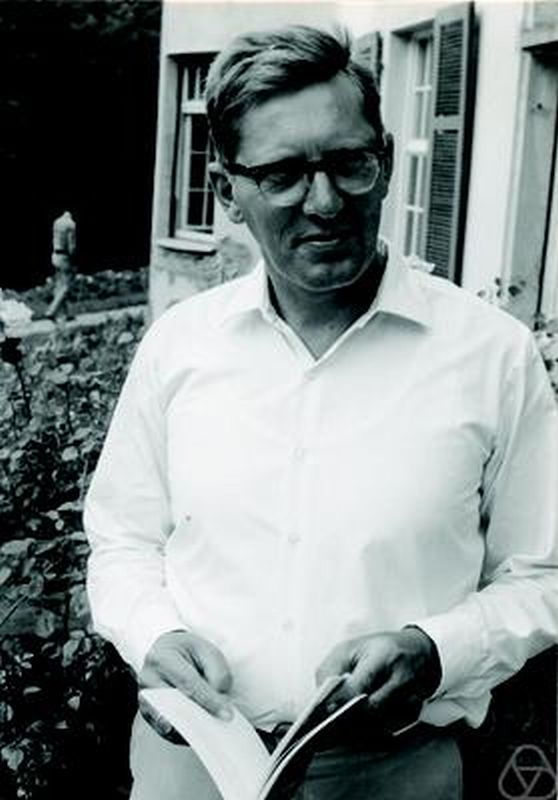
\includegraphics[trim={140pt 360pt 80pt 12pt},clip,scale=1]{deBruijn.jpg}
\\[-9em]
\end{subfigure}%
\begin{subfigure}{.6\textwidth}\small
람다식의 문법구조
{\large\[e ~::=~ x ~\mid~ \lambda x.e ~\mid~ e\;e\]}
{\footnotesize Y-combinator의 표준적 람다식 표기와}\\[1.5ex]
{\normalsize
$\phantom{.}\qquad\lambda f.(\lambda x.\,f\,(x\;x))\,(\lambda x.\,f\,(x\;x))$\\[1.25ex]
$\phantom{.}\qquad\lambda~~\,(\lambda~~2~(1~1))\,(\lambda~~2~(1~1))$}\\[1ex]
{\footnotesize 그에 상응하는 이름없는 람다식 표기}

{\footnotesize
\[
\begin{forest}
for tree={inner sep=0, l sep-=.5em, l=0}
[$\lambda f.$ [@ [$\lambda x.$ [@ [$f$] [@ [x] [x]]]]
                 [$\lambda x.$ [@ [$f$] [@ [x] [x]]]] ] ]
\end{forest}
\]
}
\end{subfigure}
\caption{람다계산법($\lambda$-calculus)의 창시자인
	 알론조 처치(Alonzo Church, 상)와
         이름없는 람다식 표기를 고안한
         니콜라스 드 브루인(Nicholaas de Bruijn, 하)
         {\scriptsize(사진 출처: MacTutor, 위키미디어 공용)}
         \label{fig:ChurchDeBruijn} }         
\end{figure}
앞서 다룬 바를 간단히 정리해 보면, $f(x) = x+x$와 $f(x) = 2\times x$는 문법구조는
다르지만 의미구조상 같고, $f(x) = x+x$와 $f(y) = y+y$는 문법구조상 본질적으로
같다고 볼 수 있다. 이름(name)을 뭐라고 부르는가는 편의상 임의로 정했을 뿐
그 자체가 본질적인 것은 아니며 오히려 이름이 어느 유효범위에
묶여있는지(name binding)의 구조가 이름의 본질이라 할 수 있다. 따라서
함수 이름 $f$를 항상 작성하는 친숙한 표기 방식은 함수의 본질만 담은
최소한의 표기는 아니다. 이러한 관점에서 알론조 처치(Alonzo Church)는
함수 $f(x) = x+x$를 이름짓지 않고 $\lambda x.x+x$와 같이 표기하는
\index{람다계산법|see{$\lambda$-calculus}}%
\index{$\lambda$-calculus|see{람다계산법}}%
람다계산법($\lambda$-calculus)을 1930년대 초에 창안\cite{Church1932}하였으며
매개변수의 이름만 바꾸면 (단, 바꾸면서 납치가 일어나지 않게) 똑같아질
수 있는 관계를 $\lambda x.x \equiv_\alpha \lambda y.y$와 같이 표기하고
\index{람다계산법!$\alpha$동치}%
\index{$\lambda$-calculus!$\alpha$-equivalence}%
\index{$\alpha$동치|see{$\alpha$-equivalence}}%
\index{$\alpha$-equivalence|see{$\alpha$동치}}%
$\alpha$동치($\alpha$-equivalence)라 불렀다.
니콜라스 드브루인(Nicholaas de Bruijn)은 람다식 문법나무에서 이름이 몇번째로
가까운 유효범위에 묶여있는지 나타내는 정수값인
\index{드브루인 인덱스|see{de Bruijn index}}%
\index{de Bruijn index|see{드브루인 인덱스}}%
드브루인 인덱스(de Bruijn index)를
이름 대신에 표시함으로써 $\alpha$동치인 람다식이 유일무이한 형태로 표기되는
람다식에 대한 이름없는 표기 방식\cite{deBruijn1972}을 고안하였다. 그러니까 람다식을
드브루인 인덱스를 활용한 표기로 바꿔봤는데 똑같다면 서로 $\alpha$동치라는 말이다.

그림\;\ref{fig:ChurchDeBruijn}에는 같은 람다식의 표준적 표기와
드브루인 인덱스를 활용한 이름없는 표기를 나란히 비교해 놓았다.
문법나무를 살펴보면,
$x$는 첫번째 가까운 $\lambda x.\cdots$로 시작하는 범위에서 나타되므로 1로,
$f$는 두번째 가까운 $\lambda f.\cdots$로 시작하는 범위에서 나타되므로 2로
표시하고 있다. 그런데 같은 이름이라도 어디에서 쓰이느냐에 따라 다른
드브루인 인덱스로 표시될 수 있다는 점에 유의하라. 예를 들어
람다식 $\lambda f.\,f\,(\lambda x.\,f\;x)$는 $\lambda~1~(\lambda~2~1)$에 상응한다.
오른쪽과 왼쪽의 $f$를 각각 1과 2의 서로 다른 드브루인 인덱스로 표시하고 있다.
왜냐하면 오른쪽 $f$가 묶여있는 $\lambda f.\cdots$는 가장 가까이 있지만
왼쪽 $f$는 $\lambda x.\cdots$ 안에 있으므로 묶여있는 곳을 찾아가려면
거기서 가장 가까운 $\lambda x.\cdots$를 거쳐 두번째로 가까운
$\lambda f.\cdots$로 가야 하기 때문이다.

람다식에 나타나는 모든 이름이 드브루인 인덱스로 변환되지는 않는다.
단적으로 이름 자체만으로 이루어진 $x$와 같은 람다식에서 이름 $x$는
드브루인 인덱스로 옮길 수 없다. 왜냐하면 이런 경우 $x$는 어디에도 묶이지
않고 자유롭기(free) 때문이다. 또한 $\lambda x.\,y\;x$의 경우도 
$\lambda~y~1$ 정도까지만 이름을 드브루인 인덱스로 변환할 수 있다.
왜냐하면 $\lambda x.\,y\;x$에서 $x$는
\index{묶인이름|see{bound name}}%
\index{bound name|see{묶인이름}}%
묶인이름(bound name)이지만
$y$는
\index{자유이름|see{free name}}%
\index{free name|see{자유이름}}%
자유이름(free name)이기 때문이다. 람다식에 자유이름이 있으면
열려있다(open)고 하고 자유이름이 없으면 닫혀있다(closed)고 한다.
보통 컴파일러의 의미분석 단계 작업의 하나로 분류되는
\index{유효범위 분석|see{scope analysis}}%
\index{scope analysis|see{유효범위 분석}}%
유효범위 분석(scope analysis)을 이런 관점에서 단순화해서 설명하면,
분석 대상이 되는 프로그램이 자유변수가 없는 닫힌 프로그램이면 통과시키고
자유변수를 포함하는 열린 프로그램이면 거부하며 오류를 내는 작업으로 볼 수 있다.

\subsection{요약문법나무 + 이름의 유효범위 묶음 = 요약묶음나무}
\index{요약문법나무}%
\index{abstract syntax tree}%
\index{AST}%
요약문법나무(abstract syntax tree, AST)에
\index{이름의 유효멈위 묶음}
\index{name binding}
이름의 유효범위 묶음(name binding)까지 표현된 구조를
\index{요약묶음나무|see{abstract binding tree}}%
\index{abstract binding tree|see{요약묶음나무}}%
\index{ABT|see{abstract binding tree}}%
\index{ABT|see{요약묶음나무}}%
요약묶음나무(abstract binding tree, ABT)라 한다 \cite{PFPL2nd}.
람다계산법(그림\;\ref{fig:ChurchDeBruijn})에서 $\lambda$와 같이
이름을 유효범위에 묶어주는 요소를 바인더(binder)라
하는데 순수한 람다식에서 바인더는 $\lambda$ 하나 뿐이다.
참고로, 여러 부분식으로 이루어지는 식을 한데 모아 복합적인(compound)
식을 구성한다는 점에서는 바인더와 같지만  이름의 유효범위 묶음을
다루지는 않는 $e_1 + e_2$에서 $+$와 같은 요소까지 아우르는 문법구조의
개념을 생성자(constructor)라고도 부른다.
실용적인 언어는 물론이고 이론적 연구 주제로 다루는 프로그래밍언어의
모형에서도 여러 종류의 바인더를 포함하는 문법구조는 드물지 않다.
요약묶음나무는 이렇게 여러 종류의 바인더를 포함한 언어의 문법구조를
다루기에 적합한 표현 방식이다.

\begin{figure}
\begin{subfigure}{.5\textwidth}
\begin{align*}
    x \in \mathcal{N} & \\
 e,e_i\in E ~&\\
   ~::=~& x \\
  ~\mid~& \bm{\lambda}\,x\,\bm{.}\;e
        & (\text{binds}~ x ~\text{in}~ e)\phantom{_{3}}\\
  ~\mid~& e_1\;e_2 \\
  ~\mid~& \textbf{let}\;x\pmb{=}e_1\;\textbf{in}\;e_2
        & (\text{binds}~ x ~\text{in}~ e_2)
\\[-5ex]
\end{align*}
\caption{Sewell 형식\label{sfig:ABTstyle1} }
\end{subfigure}
\hfill
\begin{subfigure}{.4\textwidth}
\begin{align*}
    x \in \mathcal{N} & \\
 e,e_i\in E ~&\\
   ~::=~& x \\
  ~\mid~& \bm{\lambda}(x.e) \\
  ~\mid~& \pmb{\textbf{@}}(e_1;\,e_2) \\
  ~\mid~& \textbf{let}(e_1;\,x.e_2)
\\[-5ex]
\end{align*}
\caption{Harper 형식\label{sfig:ABTstyle2} }
\end{subfigure}
\caption{요약묶음나무(ABT)의 두 가지 표현 형식\label{fig:ABTstyles}}
\end{figure}

람다식에 지역(local) 이름을 선언하는, 이를테면
$\textrm{let}\;x=3\;\textrm{in}\;x+2$를 계산한 결과가 5인,
새로운 바인더 $\textrm{let}\,\cdots\,\textrm{in}\,\cdots$으로
이루어지는 식을 추가하자.
일반적으로 let식의 형태를 $\textrm{let}\;x=e_1\;\textrm{in}\;e_2$라
하면 여기서 $e_1$은 $x$의 값을 초기화하기 위한 식일 뿐
$x$의 유효범위에 포함되지 않고 실제 $x$가 묶이는 범위는 $e_2$로 한다.
이렇게 우리말 문장으로 설명해 놓으면 어떤 이름을 어떤 유효범위에
묶는지 뜻이 전달되기는 하지만 한눈에 잘 들어오지는 않는다.
이를 그림\;\ref{fig:ABTstyles}와 같이 추상묶음나무(ABT) 형식으로 정리하여
표시하면 추상문법나무(AST)가 나타내는 문법구조의 내용과 함께
각 바인더가 어떤 이름 유효범위 묶음(name binding) 구조를 구성하는지
한눈에 들어온다. 왼쪽(그림\;\ref{sfig:ABTstyle1})은
Sewell\cite{Sewell2007ott}이 개발을 주도한 의미구조 정의
자동화 도구인 OTT의 표기와 유사한 방식이다.
OTT는 구체적문법을 처리하는 파서도 자동으로 생성하는 기능을
포함하므로 구체적문법에 가깝게 문법구조를 표현하고
바인더를 포함하는 식의 오른쪽에 이름이 묶이는 범위에
대한 부가조건을 명시한다. 오른쪽은 \citet{PFPL2nd}의 교재에 나타나는
표현 방식으로 추상문법 표현을 규격화하여 복합적인(compound) 문법요소을
만들어내는 생성자(constructor)를 앞부분(prefix)에 오도록 표현하며,
구체적문법에 나타나는 순서와 다르게 조정해서라도 이름 $x$와 그 유효범위에
해당하는 식 $e$를 항상 바로 옆에 놓고 한 덩어리로 묶어 $x.e$와
같이 표기한다. 이런 요약문법나무(ABT)로 정의된 문법구조는
납치없는 바꿔치기(capture avoiding substitution) 및
$\alpha$동치($\alpha$-equivalence) 등과 같은
이름의 유효범위 묶음(name binding)을 다루는 기본적인 연산이
제공된다고 가정한다. 실제로 ABT의 기능을 자체적으로 내장한
언어\cite{FreshML2003}나 ABT의 개념을 바탕으로 문법구조에서
이름의 유효범위를 편리하게 다루는 라이브러리\cite{Unbound2011}도
출시되어 있는데, 이런 언어나 라이브러리에서는 해당 연산을
미리 구현해 제공하거나 손쉽게 구현할 수 있는 기능을 마련하고 있다.

\section{프로그래밍언어의 타입}
\index{타입|see{type}}%
\index{type|see{타입}}%
대부분의 프로그래밍언어에는 정수, 부동소수점 수, 문자 등의
기본 타입(basic type) 혹은 원시 타입(primitive type)이 제공되며,
순서쌍, 구조체, 리스트, 배열 등 여러개의 자료를 하나로 묶는
복합 타입(compound type)이 제공된다. 또한 함수를 값으로서 다루는
프로그래밍언어에서는 함수 타입의 계산식이나 값을 직접 다룰 수 있다.
타입(type)을 `유형', `형', 또는 `꼴' 등의 우리말 용어로 옮기기도
하지만 워낙 프로그래밍 이외의 분야에서 일상용어로도 흔히 쓰는
외래어이므로 이 책에서는 그냥 `타입'이라 부르겠다.

\subsection{정적 타입과 동적 타입}\label{ssec:StaticDynamicTy}
타입은 실행 전의 프로그램식이나 계산의 진행 과정에 있는 계신식
또는 계산의 결과값을 분류하는 유형이다.
\index{정적 타입|see{static type}}%
\index{static type|see{정적 타입}}%
\index{타입!정적 타입}%
\index{type!static type}%
정적(static) 타입은 실행 전에
계산식을 미리 분류하는 개념으로, 실행 중에도 그 성질이 유지될 것을
기대하며 최종적으로 어떤 종류의 값으로 계산될지도 가늠해 볼 수 있다.
동작과정 의미구조의 관점에서 표현해 보면 다음과 같다. 실행 전에 $e:\tau$,
즉 프로그램식 $e$가 타입 $\tau$로 분류된다면, 작은걸음으로
$e\longmapsto e_1\longmapsto e_2\longmapsto\cdots$일 때
$e_1:\tau,\;e_2:\tau,\;\cdots$임을 기대하며 큰걸음으로
$e\Longmapsto v$일 때 $v:\tau$임을 기대한다는 말이다.
이렇게 정적 타입을 기반으로 한 언어에서 대표적으로 만족되기를
기대하는 실행 과정에서 타입이 유지되는 성질을
\index{타입보존|see{type preservation}}%
\index{type preservation|see{타입보존}}%
`타입보존'(type perservation)이라고 한다. 또한 잘 설계된 정적
타입 언어에서는 모든 구성 요소가 타입으로 잘 분류되는 (well-typed)
프로그램은 계산 도중에 비정상 종료되지 않고 원활히 진행(progress)되는
성질을 만족할 것도 기대한다. 정리하면, 이상적인 정적 타입 언어는
타입으로 잘 분류되는 프로그램이 실행 전에 분류된 타입대로 성질을 유지하며
원활히 계산이 진행되도록 타입 시스템이
\index{안전성|see{safety}}%
\index{안전성|see{soundness}}%
\index{safety|see{안전성}}%
\index{soundness|see{안전성}}%
안전성(safety 또는 soundness)을
보장하는 것을 추구한다. 실행 효율의 측면에서도 정적 타입 언어는
유리하다. 프로그램식이나 변수의 타입이 실행 중에 보존된다는 성질을
기대할 수 있으므로, 예를 들어 실행 전에 정수 타입으로 분류된 변수는
실행 중에 혹시 갑자기 문자열이나 함수로 내용이 바뀌지 않을까
동적 언어에서처럼 걱정하며 추가로 검사나 예외처리를 할 필요 없이
정수를 처리에 필요한 만큼만의 메모리를 배정하고 정수 타입에
최적화된 처리를 할 수 있기 때문이다.

그에 상대되는 개념인 
\index{동적 타입|see{dynamic type}}%
\index{dynamic type|see{동적 타입}}%
\index{타입!동적 타입}%
\index{type!dynamic type}%
동적(dynamic) 타입은, 더 이상 계산할 필요 없이
자명한 기본타입의 리터럴 등 일부 프로그램의 요소를 제외하고는,
일반적으로 실행 전의 프로그램식을 미리 분류하지 않고 실행하여 계산된
결과값에 대해서만 어떤 타입인지 확인하여 그 다음 계산 진행 과정에
적합한지 판단한다. 예를 들어 함수를 호출하는 위치에 해당하는 변수의
값을 계산해 그 결과를 확인해 보았는데, 결과값이 함수가 아닌 정수이거나
할 경우에는 그 다음의 계산 과정인 함수 호출이 불가능하므로 실행 오류가
발생하게 되는 것이다. 동적 언어는 이렇게 미리 오류를 검출하기 어렵고
실행 시간에 뒤늦게 오류가 드러나는 단점을 감수하고서라도 프로그래머가
표현하고자 하는 모든 정상적으로 계산 가능한 프로그램은 다 수용하겠다는
\index{완전성|see{completeness}}%
\index{completeness|see{완전성}}%
`완전성'(completeness)을 추구한다고 볼 수도 있다. 정적 타입 언어에서는
안전성을 추구하다 보니 실제로 실행해 보면 문제 없이 동작하는
일부 프로그램이 타입 시스템의 규칙에 부합하지 않는다는 이유로
바람직하지 못한 프로그램으로 취급되어 컴파일 및 실행이 거부되기도 한다.

참고로, 정적 타입을 기반으로 하는 언어에서도 동적 타입의 요소가 일부
가미되는 경우도 많다. 예를 들면 동적 디스패치를 기반으로 하는
객체지향 언어에서는 정적 타입으로 추상적인 상위 범주만 분류되고,
구체적으로 어떤 하위 범주로 분류되는 내용이 계산 과정이나 최종 결과값에
나타날지는 실행 시간에 동적 타입으로 확인가능한 경우도 있다. 그리고
조금 더 동적 타입에 가까운 요소로는 소위 리플렉션(reflection)이라 불리는,
프로그램 실행 중에 새로이 타입을 구성하는 기능을 제공하는 정적 타입 기반의
언어들도 있다. 이런 내용은 컴퓨터 관련 전공 교육과정에서 객체지향에
대한 이론을 다루거나 객체지향 언어로 실습하며 접할 기회들도 있을 것이므로
더 이상의 자세한 설명은 생략한다.

정적 타입을 기반으로 동적 타입의 요소를 가미하는 정도가 아닌,
동적 타입 언어로 작성하듯 프로그래밍할 수 있으면서 필요에 따라서
정적 타입의 기능을 일부 활용한다거나, 정적 타입 언어에서처럼
더 많은 타입 정보를 명세함으로써 더 원활한 동적 타입 언어의 활용을
꾀하는 등의 여러 가지 다양한 방식을 아울러
\index{hybrid type|see{하이브리드 타입}}%
\index{하이브리드 타입|see{hybrid type}}%
\index{타입!하이브리드 타입}
\index{type!hybrid type}
하이브리드(hybrid) 타입이라
부른다. 예를 들면 소위
\index{soft type|see{소프트 타입}}%
\index{소프트 타입|see{soft type}}%
\index{타입!하이브리드 타입!소프트 타입}%
\index{type!hybrid type!soft type}%
소프트(soft) 타입\cite{Cartwright2004soft}을
표방하는 언어 시스템은 추가적인 타입 정보를 동적 언어에 제공함으로써
실행 성능 향상을 도모하거나 실행 오류가 발생했을 때 추가적인 타입 정보를
함께 활용함으로써 더 나은 오류 처리를 도모하기는 하지만, 정적 타입의
가장 핵심적인 기능이자 장점인 실행 전에 프로그램에서 아귀가 맞지 않는
부분을 찾아 오류를 검출하는 기능을 도입하지는 않았었다. 최근 들어
업계에서도 인기가 높아지는 
\index{gradual type|see{점진적 타입}}%
\index{점진적 타입|see{gradual type}}%
\index{타입!하이브리드 타입!점진적 타입}%
\index{type!hybrid type!gradual type}%
점진적(gradual) 타입\cite{Jeremy2006gradual}을
표방하는 언어 시스템은 정적 타입 검사로 실행 전에 오류를 검출할 수
있으면서도, 기존에 동적 타입 언어로 작성된 코드를 거의 그대로 활용하며
원하는 부분에 필요한 만큼만 정적 타입을 점진적으로 적용할 수 있도록
설계되어 있다.

\subsection{요약된 의미로서의 타입}\label{sec:TypeAsAbsSem}
어떤 프로그래밍언어에 다음 기본 함수가 제공된다고 하자 (단, $\Sigma=\{a,b\}$).
\vspace{-1.5ex}
\begin{align*}
\texttt{plus} :\; & \mathbb{N} \times \mathbb{N} \to \mathbb{N} & \text{자연수의 덧셈}\\
\texttt{slen} :\; & \Sigma^{*} \to \mathbb{N} & \text{문자열의 길이}\\[-5.5ex]
\end{align*}
위의 각 함수의 지시적 의미구조는 다음과 같은 대응의 집합으로 정의하고,\vspace*{-1.5ex}
\begin{align*}
 \llbracket\,\texttt{plus}\,\rrbracket
 =~& \{ (0,0)\mapsto 0,\,
        (0,1)\mapsto 1,\,(1,0)\to 1,\,
        (0,2)\mapsto 2,\,(1,1)\mapsto 2,\,
        \ldots\,
     \}
 \\
 \llbracket\,\texttt{slen}\,\rrbracket
 =~& \{ \varepsilon\mapsto 0, 
        a\mapsto 1,\;b\mapsto 1,\;
        aa\mapsto 2,\;ab\mapsto 2,\;ba\mapsto 2,\;bb\mapsto 2,\;
        \ldots\;
     \} \\[-5.5ex]
\end{align*}
자연수나 문자열의 의미는
$\llbracket 25 \rrbracket = \{25\}$나 $\llbracket abba \rrbracket = \{abba\}$ 같이
그 값 하나만으로 이루어진 집합(singleton set)으로, 그리고 순서쌍의 의미는
각 요소 의미의 곱집합인
$\llbracket(e_1,\ldots,e_k)\rrbracket =
 \llbracket e_1\rrbracket\times\cdots\times\llbracket e_k\rrbracket$로 정의하자.
그러면 함수 호출의 의미는 다음과 같이 정의할 수 있다.\vspace*{-1ex}
\begin{quote}
$ \llbracket\,f(e_1,\ldots,e_k)\,\rrbracket
 = \{ v' \mid v \in \llbracket (e_1,\ldots,e_k)\rrbracket,\,
              v\mapsto v' \in \llbracket f\rrbracket \} $
\end{quote}
이런 의미구조는 실행했을 때 구체적으로 어떤 결과값일지 정확한 내용을
표현한다. 예컨대, 두 문자열 $ab$와 $bba$의 길이이 합을 구하는 프로그램을
지시함수 $\llbracket\cdot\rrbracket$의 정의에 따라 풀어가 보면 다음과 같다.
\vspace*{-1.5ex}
{\addtolength{\jot}{-.5ex}
\begin{align*}
  & \llbracket\,\texttt{plus}(\texttt{slen}(ab),\,\texttt{slen}(bba))\,\rrbracket \\
=~& \{ v' \mid
       v \in \llbracket\,(\texttt{slen}(ab),\,\texttt{slen}(\texttt{bba}))\,\rrbracket,\;
       v\mapsto v' \in \llbracket\texttt{plus}\rrbracket \} \\
=~& \{ v' \mid
       v \in \llbracket\texttt{slen}(ab)\rrbracket\times
             \llbracket\texttt{slen}(bba)\rrbracket,\,
       v\mapsto v' \in \llbracket\texttt{plus}\rrbracket \} \\
=~& \cdots \\
=~& \{ v' \mid
       v \in \{2\}\times\{3\},\,
       v\mapsto v' \in \llbracket\texttt{plus}\rrbracket \} \\
=~& \{ v' \mid v\in \{\,(2,\,3)\,\},~\;
       v\mapsto v' \in \llbracket\texttt{plus}\rrbracket \} \\
=~& \{5\}
\end{align*}
}

이번에는 같은 언어에 때한 다른 의미구조($\llbracket\,\cdot\,\rrbracket_t$)를
그림\;\ref{fig:AbsSemType}와 같이 정의해 보자. 가장 기본적인 값인 자연수와
문자열의 의미를 정확히 그 하나의 값으로만 이루어진 집합으로 좁히는
$\llbracket\cdot\rrbracket$과 달리, 이번에 정의한 지시함수
$\llbracket\cdot\rrbracket_t$는 크게 어림잡아 자연수 전체의 집합 $\mathbb{N}$과
문자열 전체의 집합 $\Sigma^{*}$이라는 아주 넓은 범위를 그 의미로 삼는다.
즉, 자연수끼리나 문자열끼리 구체적인 값이야 어찌되었든 의미를 구별하지 않고
뭉뚱그려 취급하는 것이다. 앞서 지시함수 $\llbracket\cdot\rrbracket$의 정의에 따라
풀어가 보았던 프로그램 $\texttt{plus}(\texttt{slen}(ab),\,\texttt{slen}(bba))$를
이번에는 $\llbracket\cdot\rrbracket_t$의 정의에 따라 풀어가 보자.
$\llbracket\texttt{slen}\rrbracket_t = \Sigma^{*}\to\mathbb{N}$이고
$\llbracket ab\rrbracket_t = \Sigma^{*}$라서
$\llbracket\texttt{slen}\rrbracket_t = \llbracket ab\rrbracket_t \to \mathbb{N}$이
성립하므로, 그림\;\ref{fig:AbsSemType}에서 마지막의 함수 호출에 대한 지시함수
정의를 적용하면 $\llbracket\texttt{slen}(ab)\rrbracket_t = \mathbb{N}$이다.
마찬가지로 $\llbracket\texttt{slen}(bba)\rrbracket_t = \mathbb{N}$이며,
따라서 $\llbracket(\texttt{slen}(ab),\texttt{slen}(bba))\rrbracket_t
                      = \mathbb{N} \times \mathbb{N}$이다.
$\llbracket\texttt{plus}\rrbracket_t = \mathbb{N}\times\mathbb{N}\to\mathbb{N}$이므로
$\llbracket\texttt{plus}\rrbracket_t
 = \llbracket(\texttt{slen}(ab),\texttt{slen}(bba))\rrbracket_t\to\mathbb{N}$이
성립하므로, 다시 함수 호출에 대한 정의를 적용하면
$\llbracket\texttt{plus}(\texttt{slen}(ab),\texttt{slen}(bba))\rrbracket_t 
 = \mathbb{N}$이 된다. 구체적 의미구조로
 $\llbracket\texttt{plus}(\texttt{slen}(ab),\texttt{slen}(bba))\rrbracket
 = \{5\}$였으므로 다음이 성립함을 알 수 있다.\vspace*{-1ex}
\begin{quote}
$\llbracket\texttt{plus}(\texttt{slen}(ab),\texttt{slen}(bba))\rrbracket \subset
 \llbracket\texttt{plus}(\texttt{slen}(ab),\texttt{slen}(bba))\rrbracket_t$
\vspace*{-1ex}
\end{quote} 
일반적으로 구체적인 의미구조로 정확히 풀이된 의미는 요약된 의미구조로
어림잡아 계산된 포괄적인 의미의 부분집합이 될 것이다
(즉, $\llbracket e\rrbracket \subset \llbracket e\rrbracket_t$).

\begin{figure}
\begin{align*}
\llbracket\,\texttt{plus}\,\rrbracket_t =~& \mathbb{N}\times\mathbb{N} \to \mathbb{N} \\
\llbracket\,\texttt{slen}\,\rrbracket_t =~& \Sigma^{*} \to \mathbb{N} \\
\llbracket\,n\,\rrbracket_t =~& \mathbb{N} \qquad (n\in\mathbb{N}) \\
\llbracket\,x\,\rrbracket_t =~& \Sigma^{*} \qquad (x\in\Sigma^{*}) \\
\llbracket\,(e_1,\ldots,e_k)\,\rrbracket_t =~& 
    \llbracket e_1\rrbracket_t\times\cdots\times\llbracket e_k\rrbracket_t \\
\llbracket\,f(e_1,\ldots,e_k)\,\rrbracket_t =~& \!\!\!\!
    \begin{cases}
     B & \llbracket\,f\,\rrbracket_t = \llbracket(e_1,\cdots,e_k)\rrbracket_t \to B\\
     \{\,\} & \text{otherwise}
    \end{cases}
\end{align*}
\caption{요약된 의미로서의 타입을 나타내는 지시적 의미구조\label{fig:AbsSemType}}
\end{figure}



방금전의 요약된 의미구조 $\llbracket\cdot\rrbracket_t$에 따른 풀이 과정은,
타입 검사 과정에서 함수에 넘어가는 인자들의 타입과 함수 파라메터의 타입이
일치하는지 확인되면 해당 함수 호출식의 타입은 결과적으로 함수의 리턴 타입으로
분류되는 타입 검사과정의 논리구조와 동일하다. 이러한 점에서 프로그래밍언어의
정적 타입 시스템은 요약된 의미구조를 구현하고 있다고 볼 수 있으며, 그런
의미에서 정적 타입 시스템을 프로그래밍언어의 정적 의미구조(static semantics)라
부르기도 한다.

\newpage

\section*{요점정리}
\begin{itemize}[itemsep=0pt]
 \item 프로그램에서 이름의 본질은 어떻게 불리냐가 아니라 이름이
       어떤 유효범위에 묶여있는지(name binding)의 구조에 있다.
 \item 이름의 유효범위를 고려하지 않고 소스코드에서 문자열을 치환하듯
       일괄적으로 이름을 바꿔치면 원래 의도했던 것보다 더 좁은 범위에
       이름이 묶여버리는 이름 납치(capture)가 발생할 수 있다.
 \item 유효범위에 묶인(bound) 이름이 아닌 어디에도 묶여있지 않은 이름을
       자유(free)이름이라 부른다. 자유이름이 있으면 열려있다(open)고
       하며 자유이름 없이 묶인이름만 있으면 닫혀있다(closed)고 한다.
 \item 프로그램에서 변수 등의 이름이 유효범위에 맞게 사용되는지
       검사하는 유효범위 분석(scope analysis)을 단순화해 설명하면,
       닫힌(closed) 프로그램은 통과시키고 열린(open) 프로그램은
       거부하며 오류를 내는 작업이다.
 \item 람다계산법은 함수에 이름을 붙이지 않고 함수의 내용을 나타내는
       표기 방식으로 알론조 처치(Alonzo Church)가 1930년대 초에
       창안하였다.
 \item 이름의 유효범위 묶음을 고려한 문법구조의 일치를
       $\alpha$동치라 부른다.
 \item 이름이 사용되는 곳에서 몇번째로 가까운 유효범위에 묶여있는지를
       나타내는 정수값을 드브로인 인덱스(de Bruijn index)라 한다.
 \item 드브로인 인덱스를 활용하면 $\alpha$동치인 람다식이 유일무이하게
       표현되는 이름없는 방식의 람다식 표기가 가능하다.
 \item 추상문법나무(AST)에 이름의 유효범위 묶음(name binding)까지
       포함된 문법구조의 표현을 추상묶음나무(ABT)라 한다.
 \item 람다식에서 $\lambda$와 같이 이름을 유효범위에 묶는 문법구조의
       요소를 바인더(binder)라고 하며, 추상묶음나무로 바인더를
       포함한 문법구조를 정의할 수 있다.
 \item 정적 타입 언어는 실행 전에 프로그램식을 타입으로 분류하므로
       일찍 오류를 검출할 수 있다. 또한 계산 과정과 최종 결과값에
       이르기까지 타입을 보존(preservation)하려 하므로 실행 성능에
       있어서도 도중에 값의 종류가 바뀔지 모르는 동적 타입 언어보다
       유리하다.
 \item 정적 타입 언어는 실행 전에 잘 분류된 프로그램 타입을
       보존(preservation)하며 비정상 종료 없는 계산의 진행(progress)을
       보장하는 타입 안전성(safety 또는 soundness)을 추구한다.
 \item 동적 타입 언어는 프로그래머가 재량껏 표현 가능한 모든
       정상 실행 가능한 프로그램을 받아들이려는 완전성(completeness)을
       추구한다고 볼 수 있다.
 \item 정적 타입은, 정확한 범위로 계산하는 구체적인 의미구조에 대비되는,
       넓게 어림잡아 계산하는 요약된 의미구조로 이해할 수도 있다.
\end{itemize}

\section*{연습문제}
~\vspace{-6ex}
\begin{multicols}{4}
  \begin{enumerate}[(1)]\tightlist
   \item $\lambda x.\lambda x.x$
   \item $\lambda x.\lambda x.y$
   \item $\lambda x.\lambda y.x$
   \item $\lambda x.\lambda y.y$
   \item $\lambda y.\lambda x.x$
   \item $\lambda y.\lambda x.y$
   \item $\lambda y.\lambda x.y$
   \item $\lambda y.\lambda y.y$
  \end{enumerate}
\end{multicols}
\begin{enumerate}
 \item 위의 각 람다식이 닫힌식인지 열린식인지 구분해 보라.
 \item 위에서 $\alpha$동치인 람다식끼리 모아 분류해 보라.
 \item 위의 각 람다식을 드브루인 인덱스를 이용한 표기로 바꾸어 보라.
\end{enumerate}

\section*{탐구과제}
\begin{enumerate}
 \item 업계에서 활용되는 점진적 타입(gradual type)에
       기반한 프로그래밍언어에 대해 조사해 보라.
\end{enumerate}

